\documentclass{report}

% --- Packages ---
\usepackage[a4paper,left=3cm,right=2.5cm,top=2.5cm,bottom=2.5cm]{geometry}
\usepackage{graphicx}
\usepackage{booktabs}
\usepackage{amsmath} 
\usepackage{caption}
\usepackage{hyperref}
\usepackage{xurl}
\usepackage[htt]{hyphenat}
\usepackage{longtable}
\usepackage{listings}
\usepackage{tikz}
\usetikzlibrary{shapes.geometric}
\usepackage{float}
\usepackage{rotating}
\usepackage{xcolor}

% Code listing style
\lstset{
  basicstyle=\small\ttfamily,
  keywords={CREATE,TABLE,VIEW,MATERIALIZED,WITH,SELECT,DISTINCT,FROM,JOIN,USING,ON,AS,GROUP,BY,SUM,COUNT,PRIMARY,KEY,AND,OR,NOT,NULL,BIGINT,INT},
  keywordstyle=\bfseries\color{blue!60!black},
  sensitive=true,
  morecomment=[l]{--},
  commentstyle=\itshape\color{gray},
  backgroundcolor=\color{gray!10},
  frame=single,
  columns=fullflexible,
  breaklines=true,
  showstringspaces=false,
  keepspaces=true,
}

% Big natural-join operator
\newcommand*{\bigbowtie}{\mathop{\vcenter{\hbox{\scalebox{1.6}{$\bowtie$}}}}\limits}

\begin{document}
\pagestyle{plain}

% --- Front ---
\pagenumbering{roman}
\begin{titlepage}
    \centering
    \vspace*{2.5cm}

    {\LARGE\bfseries Incremental View Maintenance over Tree Decompositions as SQL Views: An Evaluation on Feldera\par}

    \vspace{1.5cm}

    \vfill

    {\Large Bachelor's Thesis in Computer Science\par}
    \vspace{0.5cm}
    {\large submitted by}\\[0.3cm]
    {\Large\bfseries Ermin Mumic\par}
    {\large Matriculation number 23-705-197\par}

    \vfill

    \vspace{0.5cm}

    {\Large
    Department of Informatics\\
    University of Zurich\\[0.3cm]
    Data Systems and Theory (DaST) Group\\
    Prof.\ Dr.\ Dan Olteanu\par}

    \vspace{0.8cm}

    {\large
    Supervisor: Dr.\ Andrei Draghici\\[0.3cm]
    Submission date: 5 August 2026\par}

\end{titlepage}

\chapter*{Abstract}

In many settings, a query's result must stay current as new data arrives. Incremental view maintenance (IVM) provides this by maintaining a structure that encodes the result and updating it from each change, rather than recomputing it from scratch. Abo~Khamis et al.\ give an approach, which we call IVM$^+$, that maintains full conjunctive queries in the insert-only setting by organising the computation around a tree decomposition of the query, with a cost governed by the query's fractional hypertree width. Although the approach is theoretical, in the insert-only setting it can be expressed entirely as a set of SQL views, and so realised on top of an existing incremental engine without modifying it.

This thesis investigates whether that realisation is beneficial in practice. We build a query decomposer that rewrites a join query into the bag views of a tree decomposition, in both IVM$^+$ and an adjusted variant that drops its semijoin filters, together with a semiring extension for computing aggregates such as \texttt{COUNT}. We evaluate the rewrites on Feldera, a general-purpose incremental engine, against the baseline of maintaining the query directly, without decomposition, across graph, TPC-H and IMDB workloads.

The rewrite pays off on the queries the baseline handles worst, cyclic queries over dense data: there it maintains one query $42.96$ times faster than the baseline, at the same memory, and keeps tractable several queries the baseline cannot maintain within three hours. These gains hold even though the engine does not implement the worst-case-optimal joins the width bound assumes. Where the baseline is already cheap, on acyclic key-based joins and sparse data, the rewrite gives no speedup and adds a memory overhead of up to $2.6$ times. Within the decomposition, the final reconstruction dominates the cost and is avoidable when only the result's size is needed. Realised as plain SQL views on an unmodified engine, the IVM$^+$ decomposition is thus a worthwhile rewrite for cyclic queries over dense data, and query-shape-dependent in general.


\tableofcontents
\cleardoublepage

% --- Main Body ---
\pagenumbering{arabic} 
\chapter{Introduction}
\label{ch:introduction}

Many applications need the result of a query to stay up to date as the underlying database changes.
Recomputing that result from scratch after every change is wasteful, since each change usually affects only a small part of it.
\emph{Incremental view maintenance} (IVM) instead constructs a data structure that encodes the query result and maintains it incrementally as the database changes, so that the up-to-date result can be read from it when needed~\cite{olteanu2024IVM}.
How efficiently a query can be maintained this way depends on its structure and on the type of updates allowed.

\medskip

Abo~Khamis et al.~\cite{abokhamis2024Insert-Only} study the maintenance of \emph{full conjunctive queries}, join queries returning all attributes of the relations they combine.
We focus on the insert-only setting, in which tuples are only inserted and never deleted.
Such workloads arise in many practical settings, such as append-only event streams and continuously growing analytical datasets.
They show that in this setting a stream of inserts can be processed one tuple at a time in the same total time as evaluating the query once over the final database.
Maintaining the result incrementally is therefore essentially no more costly than computing it once.
Their approach organises this maintenance around a \emph{tree decomposition} of the query; we refer to it as the \emph{IVM$^+$ approach}.

Although the IVM$^+$ approach is theoretical in nature, in the insert-only setting it can be expressed directly as a set of SQL views.
The IVM$^+$ approach can therefore be realised on top of an existing IVM engine simply by rewriting the input query into these views, without modifying the engine itself.
This makes it lightweight to deploy, requiring only a query rewrite rather than the design or modification of a dedicated system.

\medskip

In this thesis, we investigate whether the IVM$^+$ approach is beneficial in practice when realised at the SQL level on an existing IVM engine.
We make two contributions:\footnote{The thesis repository is available at \url{https://github.com/ermin-mumic/UZH-Bachelor-Thesis-IVM}.}

\begin{itemize}
  \item \textbf{A query decomposer.} 
  We present a tool that, given a join query, computes a tree decomposition and produces the corresponding IVM$^+$ realisation as a set of SQL views.
  The entire translation is performed at the SQL level, without modifying the engine.
  The tool supports both the standard IVM$^+$ approach and an adjusted variant that we introduce in Chapter~\ref{ch:ivm}.
  It also supports aggregates such as \texttt{COUNT}, based on the concept of provenance semirings~\cite{green2007}, for both the standard approach and the variant.

  \item \textbf{An empirical evaluation on Feldera.}
  As our target engine we use Feldera~\cite{feldera2026}, a general-purpose engine based on the DBSP model~\cite{budiu2023DBSP} that incrementally maintains SQL views as the underlying data changes.
  In Feldera, queries are expressed as SQL views, which makes the rewritten IVM$^+$ views a natural fit.
  We compare the maintenance performance of the rewritten queries against that of the original queries.
\end{itemize}

Our evaluation finds that the rewrite helps most where the original query would otherwise build large intermediate results, on cyclic queries over dense data. There it maintains the result far more efficiently, in one case $42.96$ times faster than the original query and at the same memory, and it keeps tractable several queries the original cannot maintain within three hours. Where the original query is already cheap to maintain, the rewrite gives no speedup and uses up to $2.6$ times the memory, so its benefit is specific to these harder, cyclic queries rather than a property of the rewrite in general.

\medskip

The remainder of this thesis is organised as follows.
Chapter~\ref{ch:background} introduces the necessary background: the query model, the insert-only maintenance problem, tree decompositions and fractional hypertree width.
Chapter~\ref{ch:ivm} presents the IVM$^+$ approach, our adjusted variant, and a semiring extension for computing aggregates.
Chapter~\ref{ch:implementation} describes the query decomposer and the experiment harness, and how the approach is realised as Feldera views.
Chapter~\ref{ch:evaluation} reports the experimental setup, datasets, and results.
Chapter~\ref{ch:conclusion} concludes and discusses future work.

\chapter{Background}
\label{ch:background}

This chapter introduces the formal foundations underlying the IVM$^+$ approach and the adjusted variant studied in this thesis.
We first fix our data model and the class of queries we study, and introduce a running example that we revisit throughout the thesis (Section~\ref{sec:queries}).
We then introduce tree decompositions (Section~\ref{sec:tree_decompositions}), the structure the IVM$^+$ approach is organized around, and the fractional hypertree width derived from them (Section~\ref{sec:fhw}).

\section{Data Model and Queries}
\label{sec:queries}

We use standard relational terminology, which we briefly recall here~\cite{abiteboul1995}.

\medskip

A \emph{relation} $R$ is a finite set of tuples, and a \emph{database} $\mathcal{D}$ is a finite set of relations.
The \emph{size} $|R|$ of a relation is its number of tuples, and the size $|\mathcal{D}|$ of a database is the sum of the sizes of its relations.

\medskip

A \emph{full conjunctive query}, also called a \emph{natural join query}~\cite{abokhamis2024Insert-Only}, has the form
\[
Q = R_1(\mathbf{X}_1) \bowtie \cdots \bowtie R_k(\mathbf{X}_k),
\] 
where each $R_i$ is a relation symbol and each $\mathbf{X}_i$ is a tuple of variables, the \emph{schema} of $R_i$. Each $R_i(\mathbf{X}_i)$ is an \emph{atom} of $Q$, and $\mathrm{vars}(Q) = \bigcup_{i=1}^{k} \mathbf{X}_i$ denotes the set of all variables of $Q$.
We call such a query \emph{full} because every variable in $\mathrm{vars}(Q)$ is returned in the result; no variables are projected away.
For brevity we refer to full conjunctive queries simply as \emph{queries}.

A tuple $t$ over $\mathrm{vars}(Q)$ is in the \emph{result} $Q(\mathcal{D})$ if each atom $R_i(\mathbf{X}_i)$ can be matched to a tuple $t_i \in R_i$ so that the matched tuples agree on their shared variables: for every variable $x \in \mathrm{vars}(Q)$, all matched tuples $t_i$ with $x \in \mathbf{X}_i$ assign $x$ the same value, namely $t(x)$.
For a tuple $t$ and a variable $x$ in its schema, $t(x)$ denotes the value that $t$ assigns to $x$.

\paragraph{Running example.}
As a running example we use a small \emph{self-join} query over a single binary relation $E$, which we read as the edge set of a directed graph.
Consider
\[
Q_\diamond = E_1(A,B) \bowtie E_2(B,C) \bowtie E_3(C,D) \bowtie E_4(B,D) \bowtie E_5(A,D),
\]
with $\mathrm{vars}(Q_\diamond) = \{A,B,C,D\}$.
Here $E_1,\dots,E_5$ all denote the same relation $E$; we treat each atom as a distinct occurrence of $E$ over the same data, which is standard and does not affect the tree decompositions and widths defined in the following sections.
We examine its structure and tree decomposition in Section~\ref{sec:tree_decompositions} and determine its fractional hypertree width in Section~\ref{sec:fhw}; we return to $Q_\diamond$ throughout the thesis, including as a benchmark query in our experiments (Chapter~\ref{ch:evaluation}).

\section{Tree Decomposition}
\label{sec:tree_decompositions}

The structure of a query is captured by its \emph{hypergraph}: the vertices are the variables $\mathrm{vars}(Q)$, and each atom $R_i(\mathbf{X}_i)$ contributes a hyperedge on its variables $\mathbf{X}_i$.
When all atoms are binary, as in our running example, the hypergraph is an ordinary undirected graph.
For $Q_\diamond$ it is the \emph{diamond} shown in Figure~\ref{fig:diamond_hypergraph}: two triangles $\{A,B,D\}$ and $\{B,C,D\}$ sharing the edge $B\text{--}D$.

\begin{figure}[ht]
  \centering
  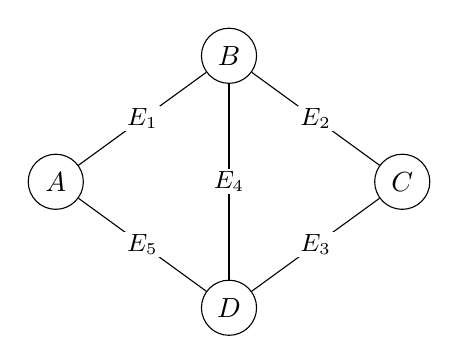
\begin{tikzpicture}[
    vertex/.style={circle, draw, minimum size=7mm, inner sep=0pt},
    lbl/.style={midway, font=\small, fill=white, inner sep=1pt}]
    \node[vertex] (B) at (0,1.6)  {$B$};
    \node[vertex] (D) at (0,-1.6) {$D$};
    \node[vertex] (A) at (-2.2,0) {$A$};
    \node[vertex] (C) at (2.2,0)  {$C$};
    \draw (A) -- (B) node[lbl] {$E_1$};
    \draw (B) -- (C) node[lbl] {$E_2$};
    \draw (C) -- (D) node[lbl] {$E_3$};
    \draw (B) -- (D) node[lbl] {$E_4$};
    \draw (A) -- (D) node[lbl] {$E_5$};
  \end{tikzpicture}
  \caption{The hypergraph of $Q_\diamond$.}
  \label{fig:diamond_hypergraph}
\end{figure}

\medskip

A \emph{tree decomposition}~\cite{cygan2015} $(\mathcal{T}, \chi)$ of a query $Q = R_1(\mathbf{X}_1) \bowtie \cdots \bowtie R_k(\mathbf{X}_k)$ consists of a rooted tree $\mathcal{T}$, whose nodes are called \emph{bags}, together with a function $\chi$ that assigns each bag $b$ a set of variables $\chi(b)$.
A valid tree decomposition satisfies two conditions:

\begin{enumerate}
    \item \textbf{Coverage:} Every atom $R_i(\mathbf{X}_i)$ is assigned to at least one bag $b$ with $\mathbf{X}_i \subseteq \chi(b)$.
    \item \textbf{Connectivity:} For every variable $x \in \mathrm{vars}(Q)$, the set of bags $\{b \mid x \in \chi(b)\}$ forms a connected subtree of $\mathcal{T}$.
\end{enumerate}

\paragraph{Running example.}
Figure~\ref{fig:diamond_td} shows a tree decomposition of $Q_\diamond$. It has two bags, one for each triangle of the hypergraph (Figure~\ref{fig:diamond_hypergraph}):
\begin{itemize}
    \item the root bag $b_1 = \{A, B, D\}$, covering the atoms $E_1(A,B)$, $E_4(B,D)$, and $E_5(A,D)$;
    \item the child bag $b_2 = \{B, C, D\}$, covering the atoms $E_2(B,C)$, $E_3(C,D)$, and $E_4(B,D)$.
\end{itemize}
Both conditions hold: every atom is covered, with the shared atom $E_4(B,D)$ lying in both bags, and every variable induces a connected subtree, since $A$ and $C$ each occur in a single bag while $B$ and $D$ occur in the two adjacent bags.
This is one of several valid tree decompositions of $Q_\diamond$; Section~\ref{sec:fhw} makes precise how their quality is measured.

\begin{figure}[ht]
  \centering
  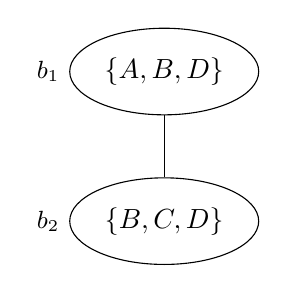
\begin{tikzpicture}[bag/.style={draw, ellipse, minimum width=24mm, minimum height=11mm, inner sep=2pt}]
    \node[bag, label={[font=\small]left:$b_1$}] (r) at (0,1.9) {$\{A,B,D\}$};
    \node[bag, label={[font=\small]left:$b_2$}] (c) at (0,0)   {$\{B,C,D\}$};
    \draw (r) -- (c);
  \end{tikzpicture}
  \caption{A tree decomposition of $Q_\diamond$.}
  \label{fig:diamond_td}
\end{figure}

\section{Fractional Hypertree Width}
\label{sec:fhw}

Let $\mathbf{V} \subseteq \mathrm{vars}(Q)$.
A \emph{fractional edge cover}~\cite{atserias2013} of $\mathbf{V}$ assigns a weight $\lambda_i \in [0,1]$ to each atom $R_i(\mathbf{X}_i)$ of $Q$ so that every variable in $\mathbf{V}$ is covered, i.e.\ the weights of the atoms whose schema contains it sum to at least one.
The \emph{fractional edge cover number} $\rho^\ast(\mathbf{V})$ is the smallest total weight of such a cover:
\[
\begin{array}{@{}ll@{\qquad}l@{}}
\text{min}   & \displaystyle \sum\nolimits_{i=1}^{k} \lambda_i & \\[8pt]
\text{s.t.} & \displaystyle \sum\nolimits_{i\,:\, x \in \mathbf{X}_i} \lambda_i \geq 1 & \forall\, x \in \mathbf{V}, \\[8pt]
                  & \lambda_i \in [0,1] & \forall\, i
\end{array}
\]
Intuitively, $\rho^\ast(\mathbf{V})$ is the least number of atoms needed to cover $\mathbf{V}$, with fractional weights allowed.

\medskip

The \emph{fractional hypertree width}~\cite{grohe2014} $w(Q)$ of $Q$ is the smallest value, over all tree decompositions $(\mathcal{T}, \chi)$, of the largest fractional edge cover number $\rho^\ast(\chi(b))$ among the bags $b$ of $\mathcal{T}$:
\[
w(Q) = \min_{(\mathcal{T}, \chi)} \; \max_{b \in \mathcal{T}} \; \rho^\ast(\chi(b)).
\]
In particular, a tree decomposition with a single bag has that bag equal to $\mathrm{vars}(Q)$, so the maximum over its bags is just $\rho^\ast(\mathrm{vars}(Q))$; since $w(Q)$ minimizes over all tree decompositions, $w(Q) \le \rho^\ast(\mathrm{vars}(Q))$.

\paragraph{Running example.}
The single-bag decomposition has $\rho^\ast(\{A,B,C,D\}) = 2$: giving $E_1(A,B)$ and $E_3(C,D)$ weight $1$ each covers all four variables, and no cover is lighter.
The two-triangle decomposition of Figure~\ref{fig:diamond_td} does better: in each triangle bag, weight $\tfrac12$ on each of its three edges covers its three variables, so $\rho^\ast(\chi(b)) = \tfrac{3}{2}$ for both bags.
No tree decomposition can do better, hence $w(Q_\diamond) = \tfrac{3}{2} < 2$.

\medskip

The IVM$^+$ approach is built on a tree decomposition of minimum fractional hypertree width, which governs the cost of maintaining the query~\cite{abokhamis2024Insert-Only}.
Computing such a decomposition is NP-hard~\cite{fischl2018}, and approximation algorithms exist~\cite{marx2010}.
Our decomposer instead uses a practical heuristic: it generates candidate decompositions with a Minimum Fill-in heuristic~\cite{bodlaender2005} and selects the one of least fractional hypertree width, as described in more detail in Chapter~\ref{ch:implementation}.


\chapter{The IVM$^+$ Approach}
\label{ch:ivm}

\section{Problem Setting}
\label{sec:ivm_problem}

We consider the \emph{insert-only} incremental view maintenance problem. The database $D$ starts empty, and a stream of $N$ single-tuple insertions arrives one at a time. After each insertion into some relation $R_i$, the maintained result $Q(D)$ must reflect the updated state. We do not consider tuple deletions.

The algorithm of Abo Khamis et al., which we call \emph{IVM$^+$}, maintains $Q(D)$ with \emph{amortized} $O(N^{w(Q)-1})$ update time per insertion, where $N$ is the current database size and $w(Q)$ is the fractional hypertree width of $Q$ (see Chapter~\ref{ch:background}). For the acyclic queries in this thesis, $w(Q) = 1$, giving $O(1)$ amortized update time per insert.

\section{Bag Relations and Bridge Variables}
\label{sec:bag_relations}

The IVM$^+$ algorithm operates on a fixed tree decomposition $\mathcal{T}$ of $Q$. We recall that each bag $t \in \mathcal{T}$ has a variable set $\chi(t)$ (see Definition~\ref{sec:tree_decompositions}). Two further notions are needed to define the algorithm's data structures.

\paragraph{Bridge variables.}
For every non-root bag $t$, the \emph{bridge variables} are the variables shared with its parent:
\[
    \mathbf{Y}_t = \chi(t) \cap \chi(\mathrm{parent}(t)).
\]
Bridge variables are the interface through which a bag communicates with its parent in the tree.c
\paragraph{Restriction of a query.}
Given a query $Q = R_1(\mathbf{X}_1) \bowtie \cdots \bowtie R_k(\mathbf{X}_k)$ and a set of variables $\mathbf{Y}$, the \emph{restriction} $Q[\mathbf{Y}]$ is the query obtained by retaining only those atoms $R_i(\mathbf{X}_i)$ for which $\mathbf{X}_i \cap \mathbf{Y} \neq \emptyset$, and projecting each such atom onto its variables in $\mathbf{Y}$:
\[
    Q[\mathbf{Y}] = \bowtie_{\,i\,:\,\mathbf{X}_i \cap \mathbf{Y} \neq \emptyset} \;\pi_{\mathbf{X}_i \cap \mathbf{Y}}\, R_i(\mathbf{X}_i).
\]
Atoms whose variable sets are disjoint from $\mathbf{Y}$ contribute nothing and are dropped. Atoms that are entirely contained in $\mathbf{Y}$ (i.e.\ $\mathbf{X}_i \subseteq \mathbf{Y}$) appear unchanged.

\paragraph{Q-relation and P-relation.}
For each bag $t$, we define two base relations:
\begin{itemize}
    \item The \textbf{Q-relation} $Q_t = Q[\chi(t)]$ is the restriction of the full query to the bag's variables.
    \item The \textbf{P-relation} $P_t = \pi_{\mathbf{Y}_t} Q_t$ is the projection of the Q-relation onto the bridge variables of $t$.
\end{itemize}
The Q-relation groups within each bag all query atoms that share variables with that bag, and the P-relation summarises which bridge variable values actually appear in the bag's result.

\section{The IVM$^+$ Algorithm}
\label{sec:ivm_algorithm}

\subsection{Q'- and P'-Relations}
\label{sec:qp_relations}

The IVM$^+$ algorithm refines the base Q- and P-relations by propagating information bottom-up through the tree. For each bag $t$, define:
\begin{align}
    Q'_t(\chi(t)) &= Q_t(\chi(t)) \;\bowtie\! \bowtie_{c \,\in\, \mathrm{children}(t)} P'_c(\mathbf{Y}_c), \label{eq:qprime} \\[4pt]
    P'_t(\mathbf{Y}_t) &= \pi_{\mathbf{Y}_t}\, Q'_t(\chi(t)). \label{eq:pprime}
\end{align}
The $Q'$-relation extends the bag's own query with the $P'$-relations of all its children. Each child's $P'$-relation acts as a \emph{semijoin filter}: it restricts the parent's join to only those bridge variable values that actually have a matching tuple somewhere in the child's subtree. The $P'$-relation of bag $t$ is then the projection of $Q'_t$ onto the bridge variables, ready to be used by $t$'s own parent.

These relations are computed \emph{bottom-up}: leaf bags have no children, so $Q'_t = Q_t$ for leaves. Once all children of a bag $t$ have their $P'$-relations, $Q'_t$ can be computed, followed immediately by $P'_t$.

\subsection{Result Reconstruction}
\label{sec:result_reconstruction}

The full query result is obtained at the root bag $r$ by joining all $Q'$-relations together along their shared variables:
\[
    Q(D) = Q'_r \;\bowtie\! \bowtie_{t \,\neq\, r} Q'_t.
\]
In practice, this is expressed as a final SQL view that joins all bag Q-views along the bridge columns.

\subsection{Complexity}
\label{sec:complexity}


\section{Variant: Without Semijoin}
\label{sec:variant_no_semijoin}

In the standard IVM$^+$ algorithm, the Q-relation $Q_t = Q[\chi(t)]$ includes \emph{all} atoms that share at least one variable with the bag, projecting each to the bag's variable set. 
We investigate a variant that adjusts this definition: the bag query retains only those atoms whose variable set \emph{contains all} bag variables, i.e.\ atoms $R_i(\mathbf{X}_i)$ for which $\chi(t) \subseteq \mathbf{X}_i$:
\[
    Q^*_t = \bowtie_{\,i\,:\,\chi(t) \subseteq \mathbf{X}_i} R_i(\mathbf{X}_i).
\]
Atoms that cover only a strict subset of $\chi(t)$ are dropped entirely rather than projected. The $Q'^*$- and $P'^*$-relations are defined analogously to Equations~\eqref{eq:qprime}--\eqref{eq:pprime} using $Q^*_t$ in place of $Q_t$.

\paragraph{Motivation.}
The projected atoms in the standard definition act as filters: they eliminate bag tuples whose bridge variable values have no matching partner in the projected relation. However, when the bridge variables are already fully constrained by another atom in the same bag, this additional filtering may be redundant, introducing join work without reducing the intermediate view size. The variant without semijoin reduction avoids this overhead by simply not including such atoms.

\paragraph{Example.}
Consider the 3-path query $Q = R(A,B) \bowtie S(B,C) \bowtie T(C,D)$ with the tree decomposition from Section~\ref{sec:tree_decompositions}. The root bag has $\chi(2) = \{B, C\}$, containing atom $S(B,C)$.

Under the \emph{standard} definition, the root Q-relation includes the projections of all atoms intersecting $\{B,C\}$:
\[
    Q_2 = \pi_B R(A,B) \;\bowtie\; S(B,C) \;\bowtie\; \pi_C T(C,D).
\]
The terms $\pi_B R$ and $\pi_C T$ are inline semijoins that restrict $S$ to bridge values seen in $R$ and $T$ respectively.

Under the \emph{variant without semijoin}, only atom $S(B,C)$ satisfies $\chi(2) = \{B,C\} \subseteq \{B,C\} = \mathbf{X}_S$; atoms $R(A,B)$ and $T(C,D)$ do not cover all of $\chi(2)$ (both are missing one variable) and are therefore dropped:
\[
    Q^*_2 = S(B,C).
\]
The root Q-view is then simply the full relation $S$, and filtering by children's bridge values is still applied via the $P'$-relations of the child bags. The trade-off between the two variants in terms of throughput and memory is evaluated in Chapter~\ref{ch:evaluation}. Prove that result still correct.

\chapter{Implementation}
\label{ch:implementation}

Chapter~\ref{ch:ivm} described the IVM$^+$ approach and its variant at the level of relational algebra, independently of any particular engine.
This chapter realises them on Feldera and presents the two tools we built: a \emph{query decomposer} and an \emph{experiment harness}.

The two share a single artifact, the set of \emph{SQL views} that encode a decomposition.
The query decomposer produces these views from an input query, and the experiment harness deploys them as a Feldera pipeline, runs it over the input data, and measures performance.
Figure~\ref{fig:ch4_overview} shows the two components.

The SQL views used in our evaluation were written by hand rather than produced by the decomposer, which we developed afterwards to generate them automatically.
They are semantically equivalent to its output and differ only in syntax.

\begin{figure}[ht]
  \centering
  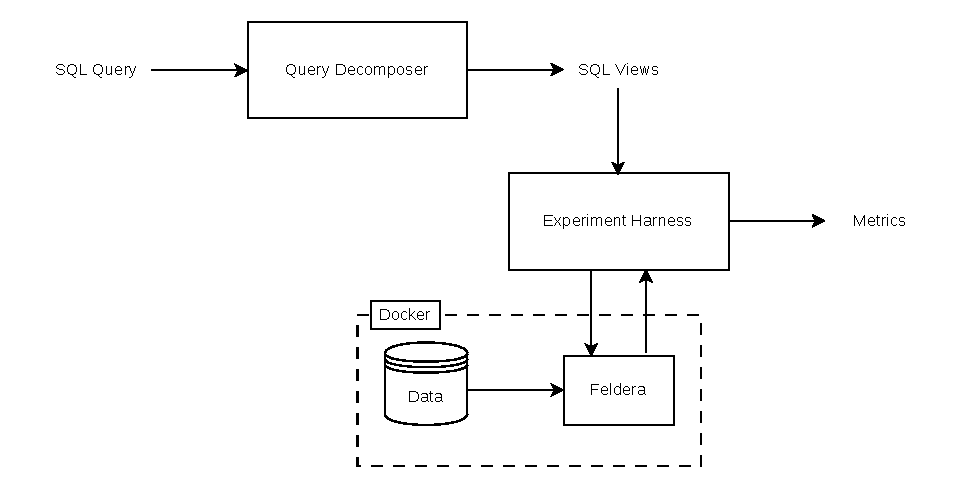
\includegraphics[width=\textwidth]{./figures/ch4_overview.pdf}
  \caption{Overview of the query decomposer and the experiment harness.}
  \label{fig:ch4_overview}
\end{figure}

We first give the necessary background on how Feldera works, then show how the decomposition of Chapter~\ref{ch:ivm} becomes a Feldera pipeline, and finally describe the decomposer and the harness in turn.

\section{Feldera}
\label{sec:feldera}

Feldera is a query engine for \emph{incremental computation}~\cite{feldera2026}.
A computation is expressed in SQL, and Feldera maintains its results as the input data changes, updating them from the changes alone rather than recomputing over all the data.
This incremental evaluation is founded on the DBSP model~\cite{budiu2023DBSP} and applies to arbitrary SQL queries.

A Feldera \emph{pipeline} is a set of SQL tables and views~\cite{feldera2026}.
The tables are the inputs, and the views are derived from them and can be nested within one another.
As changes arrive at the tables, Feldera updates every view accordingly.
This maps directly onto the construction of Chapter~\ref{ch:ivm}: the bag relations become SQL views, defined bottom-up from the base tables and the child bags' views, so the IVM$^+$ approach and its variant run as an ordinary Feldera pipeline on an unmodified engine.

Changes reach a pipeline's tables in three ways: through \emph{input connectors} attached to the tables, through HTTP requests, or through ad-hoc \texttt{INSERT} statements~\cite{feldera2026}.
Our experiments use input connectors, which read the input data from CSV files.
We chose them over HTTP ingress, which in our tests was slow enough to make ingestion, rather than the incremental computation, the bottleneck.

By default, Feldera stores only the data needed to compute future outputs, not the complete contents of every table and view~\cite{feldera2026}.
A table or view can be declared \emph{materialized} to keep its full contents available, for example to inspect or query them directly.
A table with a \texttt{PRIMARY KEY} is materialized automatically, since Feldera must maintain a key index.
Materializing a table or view can slow the pipeline down, as more data must be written to storage, which can also increase the pipeline's memory use.

\section{Decomposition as a Feldera Pipeline}
\label{sec:pipeline}

This section realises the construction of Chapter~\ref{ch:ivm} as a Feldera pipeline.
Each bag becomes a \emph{$Q'$-view} for its $Q'$-relation and a \emph{$P'$-view} for its $P'$-relation.
The views are built bottom-up, so a child's $P'$-view is ready when its parent's $Q'$-view is computed, and a final \texttt{RESULT} view produces the query's output.
We name a non-root bag's views \texttt{BAG\_N\_QPRIME} and \texttt{BAG\_N\_PPRIME}, and the root's \texttt{ROOT\_QPRIME}.
IVM$^+$ and the variant differ only in how the $Q'$-view is defined.
The view definitions are ordinary SQL, and only the input connectors and the materialisation annotations on the tables are specific to Feldera.

\subsection{Tables and connectors}

The base tables carry a Feldera \emph{input connector} that specifies where the pipeline reads its data.
For $Q_\diamond$, whose five atoms are all occurrences of one edge relation, this is a single table \texttt{EDGES(src, tgt)} with a connector that reads a CSV file:

\begin{lstlisting}[caption={The \texttt{EDGES} table with a CSV input connector.}]
CREATE TABLE EDGES (
    src BIGINT,
    tgt BIGINT
) WITH (
    'materialized' = 'true',
    'connectors' = '[{
        "transport": {
            "name": "file_input",
            "config": { 
                "path": "edges.csv" 
                } 
        },
        "format": { 
            "name": "csv", 
            "config": { 
                "headers": true 
            } 
        }
    }]'
);
\end{lstlisting}

Besides the connector, the table is declared \texttt{'materialized'}, the annotation from Section~\ref{sec:feldera} that keeps its full contents available.
The connector and this annotation are the only Feldera-specific parts of the declaration.
The views built on the table, described next, are ordinary SQL.

\subsection{Bag views}

A bag's \emph{$P'$-view} projects its \emph{$Q'$-view} onto the bridge variables, giving the set of bridge values with which the parent filters its own tuples (Chapter~\ref{ch:ivm}).
Here SQL's bag semantics matter: a plain projection keeps duplicate rows, but the $P'$-relation must be a \emph{set}, or the duplicates would multiply the parent's tuples when it joins with the view.
We therefore use \texttt{SELECT DISTINCT}.
For $Q_\diamond$, the child bag $b_2 = \{B,C,D\}$ shares $\{B,D\}$ with the root, so its $P'$-view is:

\begin{lstlisting}[caption={The $P'$-view of the child bag $b_2$.}]
CREATE MATERIALIZED VIEW BAG_2_PPRIME AS
SELECT DISTINCT B, D
FROM BAG_2_QPRIME;
\end{lstlisting}

The view is materialized and can therefore be queried directly (Section~\ref{sec:feldera}).
The $Q'$-view \texttt{BAG\_2\_QPRIME} it reads from is defined next.

We define a bag's $Q'$-view by joining its atoms on their shared variables with \texttt{USING}.
Unlike an \texttt{ON} join, \texttt{USING} merges each pair of shared columns into one, so \texttt{SELECT *} returns exactly the bag's variables and the views chain cleanly.
Because $Q_\diamond$ is a self-join, with every atom an occurrence of the same \texttt{EDGES} relation, each atom is written as a subquery that renames \texttt{src} and \texttt{tgt} to that atom's variables.
For IVM$^+$, a partially overlapping atom is added as an inline \texttt{SELECT DISTINCT} semijoin.
The child bag $b_2$ is a leaf, so its $Q'$-view is just its atoms:

\begin{lstlisting}[caption={The $Q'$-view of the child bag $b_2$ (IVM$^+$).}]
CREATE MATERIALIZED VIEW BAG_2_QPRIME AS
SELECT *
FROM (SELECT src AS B, tgt AS C FROM EDGES)
JOIN (SELECT src AS C, tgt AS D FROM EDGES) USING (C)
JOIN (SELECT src AS B, tgt AS D FROM EDGES) USING (B, D)
JOIN (SELECT DISTINCT tgt AS B FROM EDGES) USING (B)
JOIN (SELECT DISTINCT tgt AS D FROM EDGES) USING (D);
\end{lstlisting}

The first three subqueries are the contained atoms $E_2(B,C)$, $E_3(C,D)$, and $E_4(B,D)$, joined on their shared variables.
The last two are the semijoins $\pi_B E_1$ and $\pi_D E_5$, restricting $B$ and $D$ to values that occur in those atoms.
The variant keeps only the fully contained atoms and drops the two semijoins:

\begin{lstlisting}[caption={The $Q'$-view of the child bag $b_2$ (variant).}]
CREATE MATERIALIZED VIEW BAG_2_QPRIME AS
SELECT *
FROM (SELECT src AS B, tgt AS C FROM EDGES)
JOIN (SELECT src AS C, tgt AS D FROM EDGES) USING (C)
JOIN (SELECT src AS B, tgt AS D FROM EDGES) USING (B, D);
\end{lstlisting}

A non-leaf bag is built the same way but also joins its children's $P'$-views on the bridge variables.
The root's $Q'$-view \texttt{ROOT\_QPRIME}, for example, joins \texttt{BAG\_2\_PPRIME} using $\{B,D\}$.

\subsection{Result reconstruction}

The full query result is reconstructed by joining all the $Q'$-views on their shared variables (Chapter~\ref{ch:ivm}).
For $Q_\diamond$ this is a single join of the root and child $Q'$-views on the bridge variables $\{B,D\}$:

\begin{lstlisting}[caption={The \texttt{RESULT} view reconstructing the full output.}]
CREATE MATERIALIZED VIEW RESULT AS
SELECT *
FROM ROOT_QPRIME
JOIN BAG_2_QPRIME USING (B, D);
\end{lstlisting}

This \texttt{RESULT} view is the terminal view an experiment measures.
We also consider a variant \emph{without reconstruction} that omits this final join: the root's $Q'$-view \texttt{ROOT\_QPRIME} is the terminal view instead.
This isolates the cost of maintaining the bag views from the cost of joining them back into the full result.
For aggregate queries the terminal view is neither of these, but the aggregate itself, computed as described next.

\subsection{Computing \texttt{COUNT(*)}}

The number of result tuples returned by \texttt{COUNT(*)} can be computed directly on the decomposition, without materialising the full result (Section~\ref{sec:semiring}).
Each $P'$-view then carries a \emph{count} beside its bridge variables: instead of \texttt{SELECT DISTINCT}, it groups by the bridge variables and records how many tuples fall in each group.
A leaf bag's count is \texttt{COUNT(*)}: every tuple has an implicit count of one, so counting the rows in each group gives its count, with no explicit sum.
A bag with children instead multiplies its children's counts and sums the products within each group.
For $Q_\diamond$, the child bag $b_2$ is a leaf, so its $P'$-view groups by $\{B,D\}$ and counts:

\begin{lstlisting}[caption={The $P'$-view of the child bag, carrying a count.}]
CREATE MATERIALIZED VIEW BAG_2_PPRIME AS
SELECT B, D, COUNT(*) AS ANNOTATION_2
FROM BAG_2_QPRIME
GROUP BY B, D;
\end{lstlisting}

The root's $Q'$-view joins this $P'$-view as before, and so carries the column \texttt{ANNOTATION\_2}.
The \texttt{RESULT} view is then the sum over the root's $Q'$-view of the counts contributed by its child:

\begin{lstlisting}[caption={The \texttt{RESULT} view computing \texttt{COUNT(*)}.}]
CREATE MATERIALIZED VIEW RESULT AS
SELECT SUM(ANNOTATION_2) AS RESULT
FROM ROOT_QPRIME;
\end{lstlisting}

This \texttt{RESULT} is the number of tuples in the result of $Q_\diamond$, which is its \texttt{COUNT(*)}.
Because every input tuple has an implicit annotation of one, the base tables need no annotation column, and an atom appearing in several bags is not double-counted, since multiplying by one changes nothing.
An aggregate that reads a column, such as \texttt{MIN}, has no such implicit annotation: each relation must then carry its value explicitly and be counted in a single \emph{canonical} bag, or its value would be combined more than once.
We therefore implement only \texttt{COUNT(*)}.

\section{Query Decomposer}
\label{sec:decomposer}

Section~\ref{sec:pipeline} built the SQL views for $Q_\diamond$ by hand.
The \emph{query decomposer} automates this: given a query, it computes a tree decomposition and emits the corresponding $Q'$- and $P'$-views, in both the IVM$^+$ and the variant form.
It is the tool one would run to obtain a pipeline for a new query, without working through the decomposition by hand.

The decomposer takes two inputs, the query and the schema of the tables it refers to, and returns the set of SQL views.
It proceeds in four stages, shown in Figure~\ref{fig:decomposer}: a \emph{parser} reads the SQL, a \emph{hypergraph} is built from the query, a tree \emph{decomposition} is computed over it, and a \emph{generator} emits the views.
We describe each stage in turn.

\begin{figure}[ht]
  \centering
  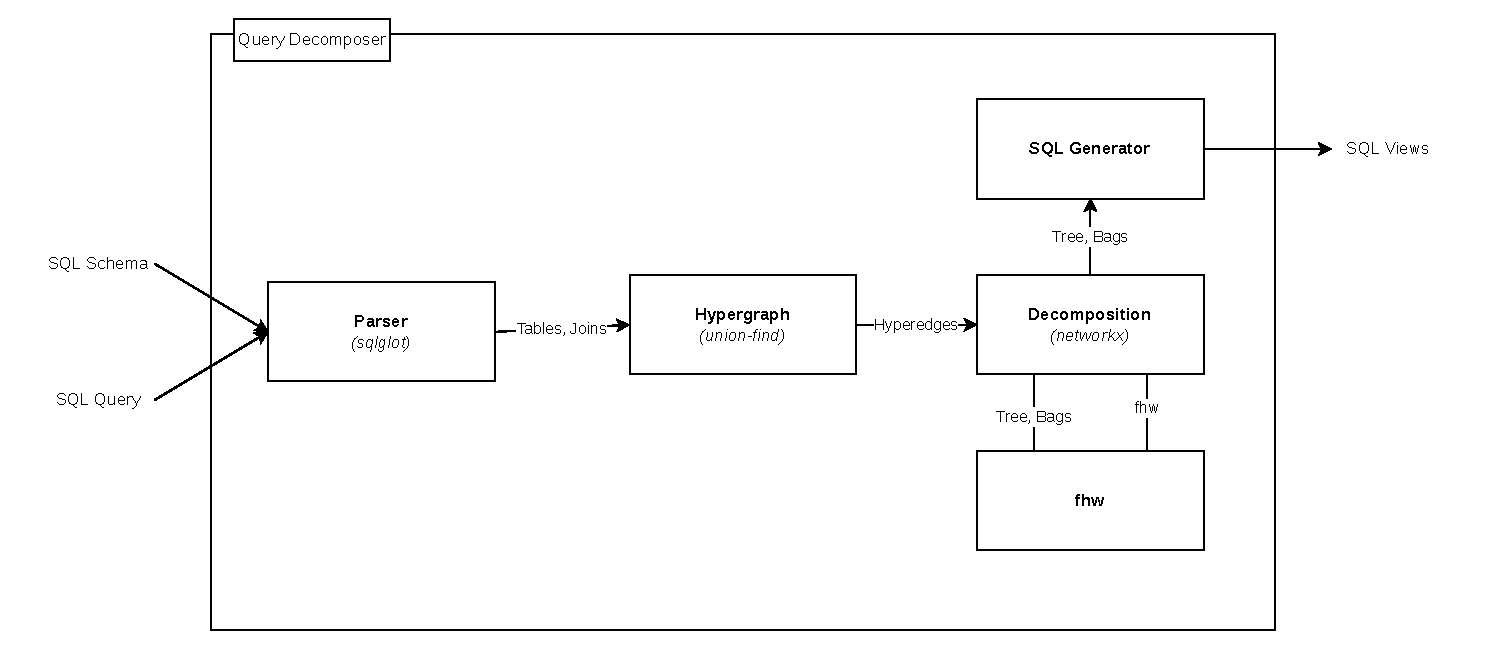
\includegraphics[width=\textwidth]{./figures/ch4_query_decomposer.pdf}
  \caption{The stages of the query decomposer.}
  \label{fig:decomposer}
\end{figure}

\subsection{Parser}

The parser reads the two SQL inputs, the schema and the query, and extracts the structure the later stages work on.
It needs the full schema, not just the query, for two reasons.
First, the tool returns the full conjunctive query, so it must know every attribute of every relation, including those the query never mentions.
Second, the hypergraph has one vertex per variable, so all variables must be known even where the query does not reference them.
Parsing itself uses \emph{sqlglot}, which turns the SQL into an abstract syntax tree that we then traverse.

The parser traverses the syntax tree clause by clause.
It first reads the \texttt{SELECT} clause, which fixes whether the query asks for the full result or a \texttt{COUNT(*)}.
It then walks the \texttt{FROM} clause and each \texttt{JOIN} clause in turn, and as it reaches a table it registers it, resolving its alias and recording its variables.
SQL lets a query rename tables and columns and use the same relation more than once, so a self-join, where one relation appears under several aliases, is registered as several independent relations, matching the atoms of Section~\ref{sec:queries}: the five occurrences of \texttt{EDGES} in $Q_\diamond$ become five relations $E_1,\dots,E_5$.
In the same pass it reads each join's equi-join condition, written as \texttt{JOIN \ldots ON} or \texttt{JOIN \ldots USING}, telling the next stage which columns are equated and therefore collapse into a single vertex of the hypergraph, even where those columns have different names.
Finally it reads the \texttt{WHERE} clause, collecting any single-relation filters.
The relations, their variables, the join conditions, and the single-relation filters are then passed on to the later stages.
The queries the parser accepts, and what it rejects, are set out in Section~\ref{sec:decomposer_limits}.

\subsection{Hypergraph}

The hypergraph stage builds the query's hypergraph, defined in Section~\ref{sec:tree_decompositions}: its vertices are the query's variables and each relation contributes one hyperedge.
A \emph{column} is an attribute of a relation in the SQL text, while a \emph{variable} is a vertex of the hypergraph, and a single variable can stand for several columns.
As noted above, an equi-join can equate two columns that do not share a name, and equated columns denote the same variable, so they must collapse into one.
The stage computes this with a \emph{union-find} structure: every column starts in its own group, each join condition merges the groups of the two columns it equates, and each final group is one variable.
Merging groups rather than pairs handles chains of joins, where equating $A=B$ and $B=C$ places all three columns in one variable.
Each variable takes its name from one of its columns, so two different variables would clash when their columns happen to share a name although no join equates them.
The stage renames such variables to keep every name distinct.
It also records, in both directions, which column of each relation a variable stands for, since the generator later needs to recover the physical column behind each variable.
Each relation then contributes one hyperedge, the set of variables of its columns.
For $Q_\diamond$ this yields the four variables $A,B,C,D$ and five hyperedges, the diamond of Figure~\ref{fig:diamond_hypergraph}, which is passed to the decomposition stage.

\subsection{Decomposition}

Section~\ref{sec:fhw} noted that computing a tree decomposition of minimum fractional hypertree width is NP-hard, so the decomposer uses a heuristic instead.
It relies on the Minimum Fill-in heuristic from the \emph{networkx} library, which operates on ordinary graphs rather than hypergraphs, so the stage first builds the \emph{primal graph} of the hypergraph: each hyperedge, that is each relation's set of variables, becomes a clique.
Making every hyperedge a clique forces its variables into a common bag, so a tree decomposition of the primal graph is a tree decomposition of the hypergraph~\cite{grohe2014}.

Minimum Fill-in is a vertex-elimination heuristic for finding a decomposition of small treewidth~\cite{bodlaender2005}.
It repeatedly eliminates the vertex whose neighbourhood is closest to a clique, measured by its number of \emph{fill-in edges}, the edges missing among its neighbours that would make them pairwise adjacent.
A vertex whose neighbours are already pairwise adjacent has no fill-in.
To eliminate a vertex the heuristic adds those missing edges, making its neighbours a clique, records the vertex together with its neighbours as a bag, and removes the vertex and its incident edges.
From these bags networkx forms the tree.
The stage then removes any bag contained in a neighbouring bag, so that none is redundant.

A single run of Minimum Fill-in produces one decomposition.
When several vertices tie for the fewest fill-in edges, the networkx implementation breaks the tie by the order in which the vertices were inserted into the primal graph.
The decomposer exploits this to obtain several candidates: it runs Minimum Fill-in once for each of a number of insertion orderings, a sorted baseline and twenty seeded shuffles, so that different tie-breaks yield different decompositions.

Minimum Fill-in targets small treewidth, but the IVM$^+$ approach wants small fractional hypertree width (Section~\ref{sec:fhw}).
The two are related: the fractional hypertree width of a query is at most its treewidth plus one~\cite{grohe2014}, so decompositions of small treewidth are a good source of ones of small fractional hypertree width.
But two decompositions of equal treewidth can still differ in fractional hypertree width, so the decomposer computes it for each candidate and keeps the smallest, breaking ties by treewidth.
The fractional hypertree width of a candidate is the largest fractional edge cover number over its bags, obtained by solving the linear program of Section~\ref{sec:fhw} with \emph{scipy}.
For $Q_\diamond$ this selects the two-triangle decomposition of Figure~\ref{fig:diamond_td}, of fractional hypertree width $\tfrac{3}{2}$.
The selected bags and tree are passed to the SQL generator.

\subsection{SQL generator}

The generator turns the bags and tree from the previous stage into the SQL views of Section~\ref{sec:pipeline}, producing automatically the translation presented there for $Q_\diamond$.
It first \emph{orients} the tree by choosing a root, by default bag~1, though any bag may serve as root, which gives every bag a parent and a set of children.
For each non-root bag it then computes the \emph{bridge variables} it shares with its parent.

The views are emitted bottom-up, each bag after its children, so a child's $P'$-view is ready when its parent needs it, matching the construction of Section~\ref{sec:pipeline}.
For a bag, the generator builds its $Q'$-view from the atoms.
Each atom becomes a subquery over its underlying table: using the mapping the hypergraph stage recorded, the generator selects the physical column each of the bag's variables stands for and aliases it to the variable, as in the \texttt{src AS B} of Section~\ref{sec:pipeline}, and appends the atom's single-relation filters as a \texttt{WHERE} clause.
The subqueries are joined with \texttt{JOIN \ldots USING} on their shared variables.
IVM$^+$ and the variant differ only here, in that IVM$^+$ adds a partially overlapping atom as a \texttt{SELECT DISTINCT} semijoin while the variant drops it (Section~\ref{sec:pipeline}).
The $Q'$-view is completed by joining the $P'$-views of the bag's children on the bridge variables, and the generator joins only on variables the view already contains, so it never references a column that is not there.
For a non-root bag it also emits the $P'$-view.

Finally the generator emits the \texttt{RESULT} view, the reconstruction join of all the $Q'$-views for a full-result query, or the single \texttt{COUNT(*)} scalar for an aggregate.
For $Q_\diamond$ the generator produces the views of Section~\ref{sec:pipeline}, up to the tool's own bag numbering.

The decomposer exposes two choices, each of which regenerates the views: switching between IVM$^+$ and the variant, and re-rooting the tree at a different bag.
Re-rooting changes the parent--child structure of the bags, and so the views and the size of the intermediate results they hold, even though the final result is unchanged.
How the orientation affects performance is examined in Chapter~\ref{ch:evaluation}, where we compare several orientations of the same query.

Figure~\ref{fig:decomposer_ui} shows the decomposer's web interface on $Q_\diamond$.
The schema and the query are entered at the top, on the left and right, and pressing \emph{Decompose} fills in the lower half.
On the left, the tree decomposition is drawn with each bag's number and variables and each edge's bridge variables, above a menu that selects the root.
On the right are the generated views, with a toggle between IVM$^+$ and the variant.
The interface labels the variant \texttt{IVM+*}~(strict), and the figure shows it, rooted at $\{A,B,D\}$ as in our example.
The tool assigns its own bag numbers, so the child bag $b_2$ appears here as \texttt{BAG\_1}.

\begin{figure}[H]
  \centering
  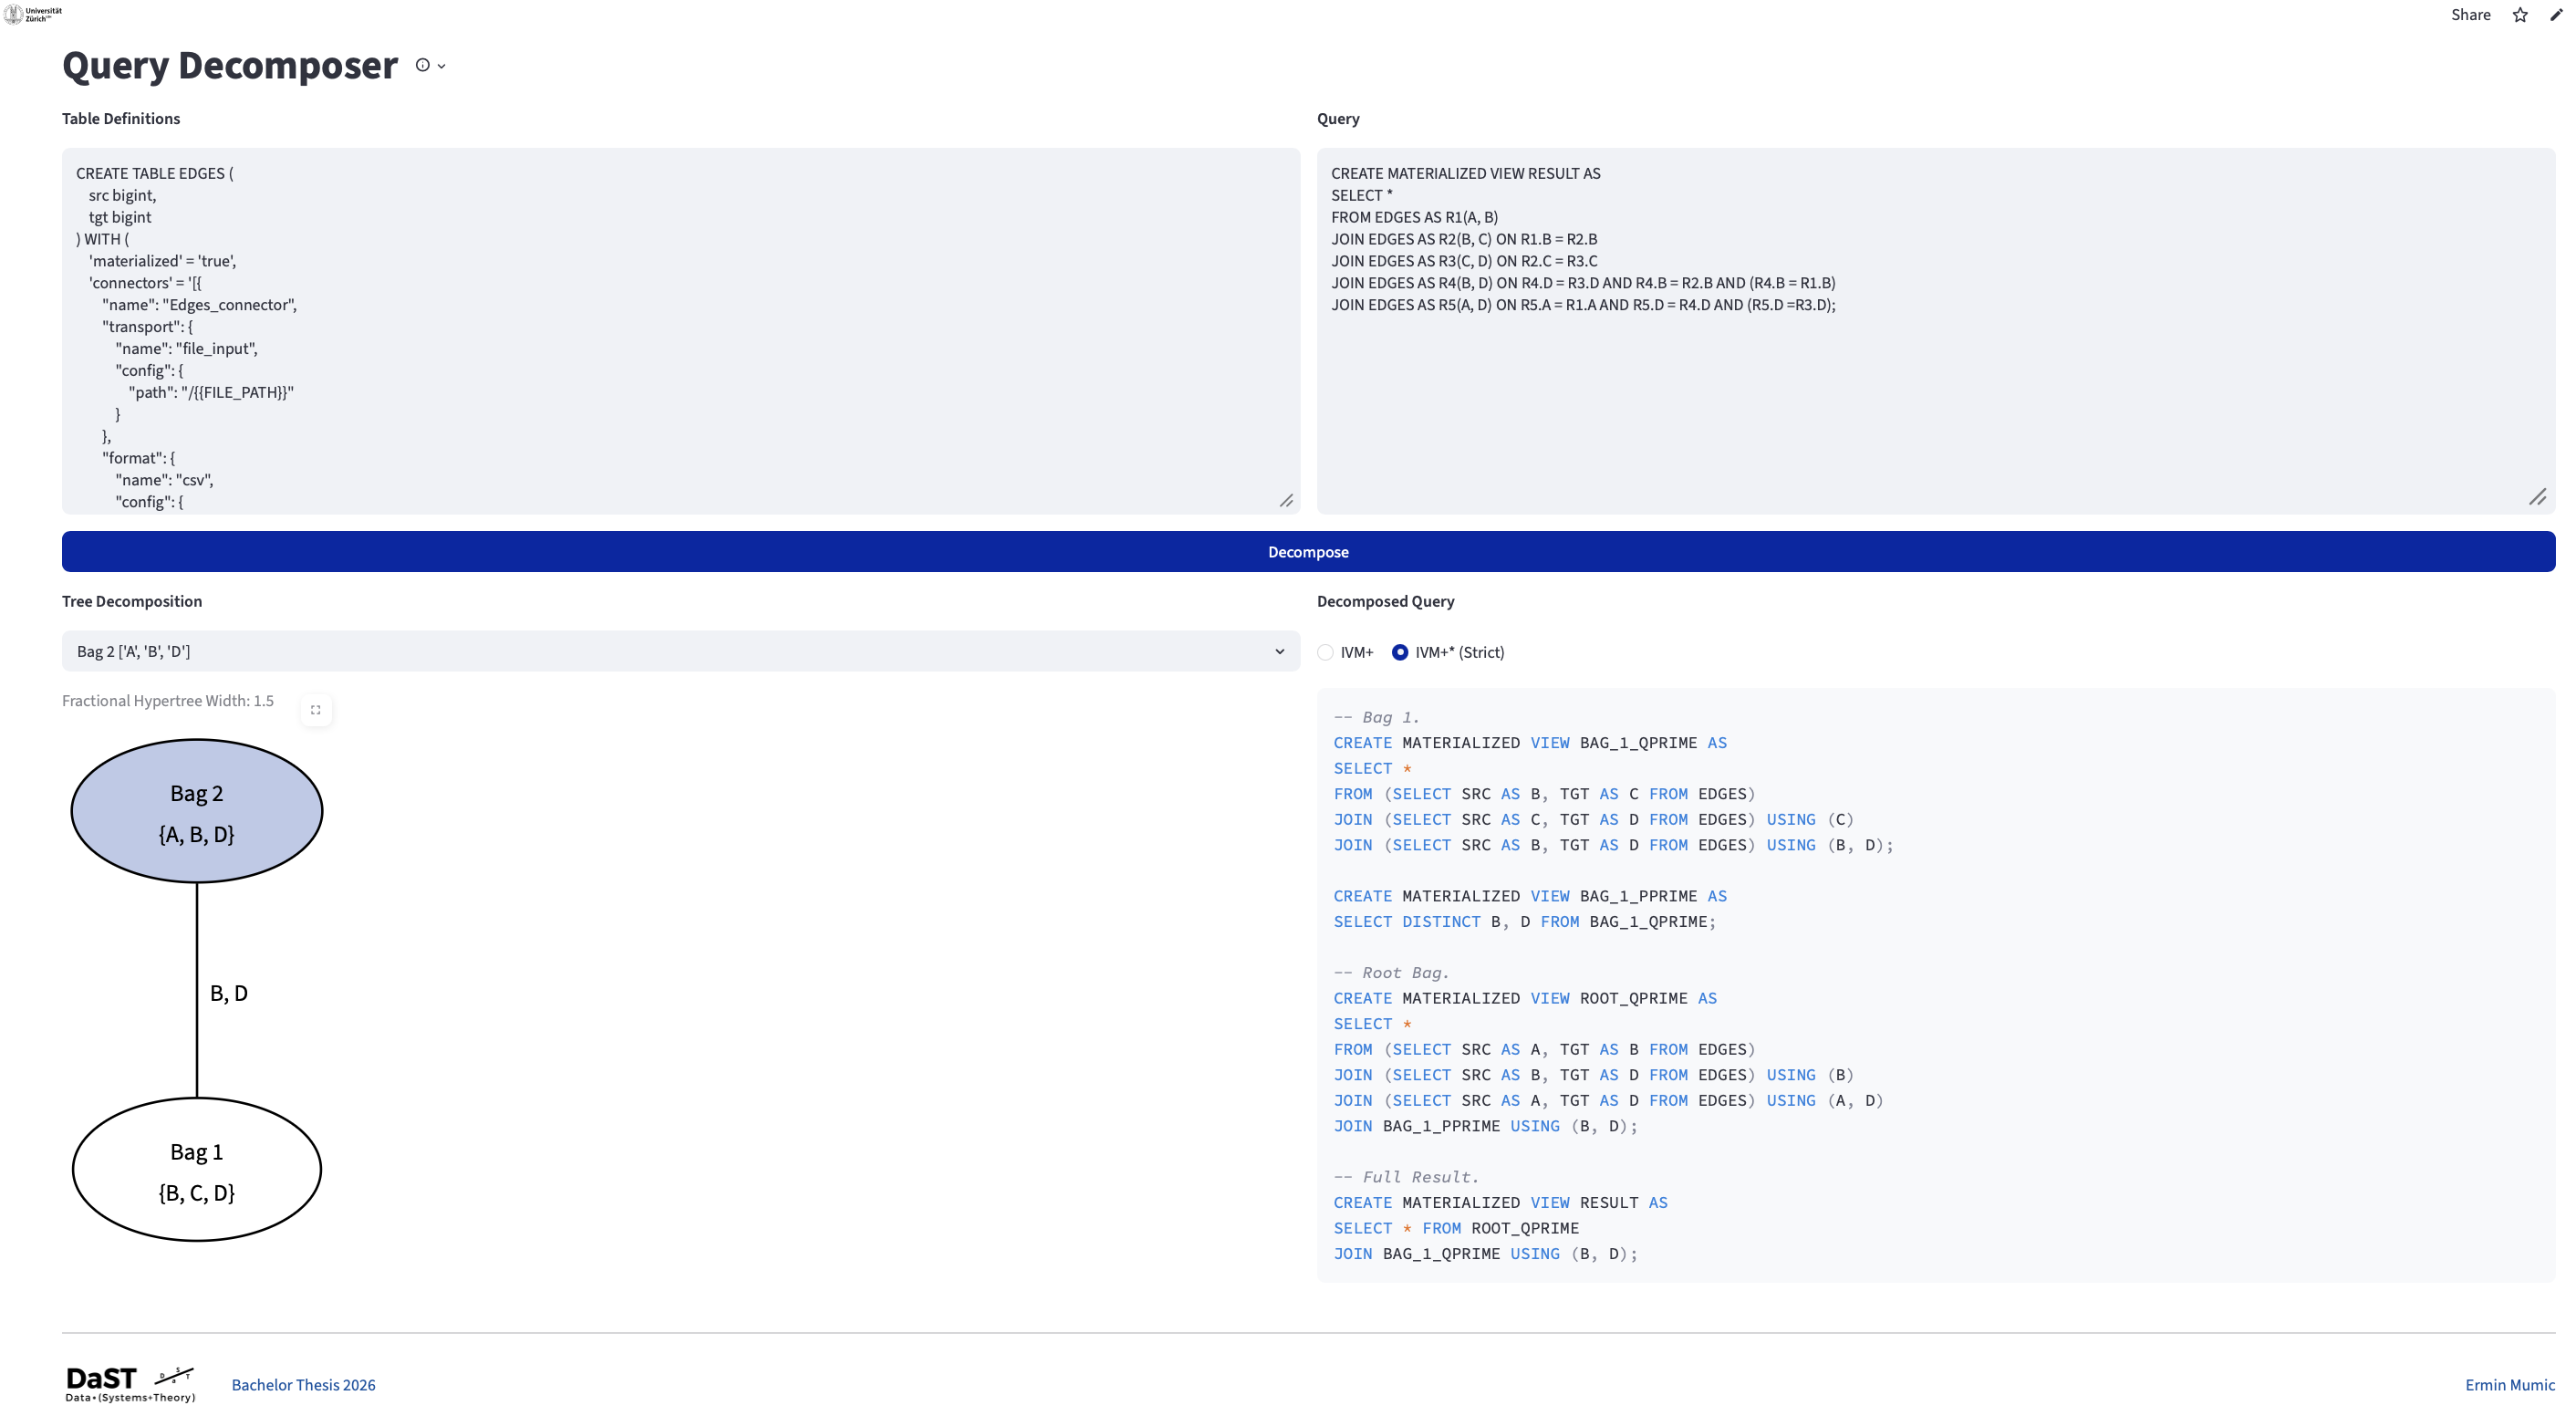
\includegraphics[width=\textwidth]{./figures/ch4_web_ui.png}
  \caption{The query decomposer's web interface on $Q_\diamond$.}
  \label{fig:decomposer_ui}
\end{figure}

These views are the artifact the experiment harness deploys.

\subsection{Supported queries and limitations}
\label{sec:decomposer_limits}

The decomposer handles \emph{full conjunctive queries} over an input schema, the class the IVM$^+$ approach targets.
The schema is given as \texttt{CREATE TABLE} statements, of which the parser reads only the column definitions and ignores the rest, so the Feldera-specific connector and materialisation annotations of Section~\ref{sec:pipeline} may be left in place and the same schema used for a pipeline can be handed to the decomposer unchanged.

A query must be a single \texttt{SELECT *} or \texttt{SELECT COUNT(*)}.
In both cases the decomposer emits the bag views and a final \texttt{RESULT} view.
For \texttt{SELECT *} the \texttt{RESULT} view reconstructs the full join, and for \texttt{SELECT COUNT(*)} it returns the count, computed on the decomposition by the semiring aggregate of Section~\ref{sec:pipeline}.
Tables and columns may be aliased, and a relation may occur several times, so self-joins such as $Q_\diamond$ are supported, written either \texttt{EDGES AS R1} or with a renamed column list \texttt{EDGES AS R1(A, B)}.
Joins must be equi-joins, written \texttt{JOIN \ldots ON $c_1$ = $c_2$} or \texttt{JOIN \ldots USING}.
The \texttt{WHERE} clause may carry filters that each reference a single relation, combined with \texttt{AND}, and each such filter is pushed into that relation's subquery.

\medskip

Everything outside this class is rejected or unsupported.
\texttt{COUNT(*)} is the only aggregate, and other aggregates and projections of specific columns are not available.
Only equi-joins are recognised, so inequality and outer joins are not supported.
A \texttt{WHERE} condition that spans more than one relation is rejected, whether a comparison between columns of different relations or a disjunction across them.
A filter on each relation separately, joined by \texttt{AND}, is the supported form.
Subqueries are not supported.

Finally, the decomposer performs only the checks its translation needs and is not a full SQL validator.
A query should therefore be validated in a database engine, for instance Feldera itself, before it is given to the decomposer.

\bigskip

In this chapter, we detail the implementation of the components required to evaluate the theoretical IVM$^+$ approach in practice. This includes the manual translation of tree decompositions into Feldera SQL pipelines, as well as the development of an automated, multi-threaded benchmarking harness designed to orchestrate the experiments.
\paragraph{Materialization policy.}
Feldera materializes a relation only when explicitly requested, and materializes a
base table automatically when a \texttt{PRIMARY KEY} is declared, since it must
maintain a key index. Materialization additionally stores a relation's full
contents so it can be queried at runtime; it is a storage feature rather than a
performance optimization. To keep the comparison fair, we hold materialization
identical across all variants except for the single view whose output each
experiment reads. All base tables use the same schema in every variant, so any
storage they incur (for example, from primary keys) is constant across the
baseline and the IVM$^+$ configurations and cancels out of the comparison. Among
the derived views we materialize only the terminal view that an experiment
measures --- the reconstructed \texttt{RESULT} for the baseline and the rejoining
variant, and the root bag for the non-rejoining variant --- and leave all
intermediate bag views non-materialized. We keep the terminal view materialized so
that Feldera does not prune the computation that feeds it.

final result reconstruction throug:In practice, this is expressed as a final SQL view that joins all bag Q-views along the bridge columns.

\section{IVM$^+$ Translation and Pipeline Construction}
\label{sec:manual_translation}

Each experimental query variant is expressed as a self-contained Feldera SQL file that defines both the input schema with its data connectors and the sequence of materialized views encoding the query logic. All files are parameterized templates: the literal \texttt{\{\{FILE\_PATH\}\}} is substituted at runtime by the benchmarking harness (see Section~\ref{sec:benchmark_harness}) with the actual dataset path, allowing the same pipeline definition to run against multiple datasets without modification, provided they conform to the same relational schema (e.g., executing the same TPC-H query template across Scale Factors 1, 10, and 30).

\subsection{IVM$^+$ Decomposition Translation}
\label{sec:decomposition_translation}

The IVM$^+$ algorithm (see Chapter~\ref{ch:ivm}) operates on a tree decomposition of the query hypergraph. Each node of the decomposition tree is a \emph{bag} that groups a subset of the query relations. Translating this structure into Feldera SQL, every bag is represented by a pair of materialized views, which instruct the DBSP engine to physically store and incrementally update the view's contents after every insert.:

\begin{itemize}
    \item \textbf{Q-view} (\texttt{CHILD\_N\_Q}, \texttt{ROOT\_Q}): corresponding to the $Q'$-relation in the theoretical formulation.
    \item \textbf{P-view} (\texttt{CHILD\_N\_P}): computed as \texttt{SELECT DISTINCT} over the join attributes. This corresponds to the $P'$-relation.
\end{itemize}

Views are defined bottom-up following the tree structure, so each child's P-view is available when the parent's Q-view is computed. The final \texttt{RESULT} view reconstructs the full output by joining all Q-views back together.

For multi-relation schemas, we use \texttt{JOIN \ldots USING} rather than explicit \texttt{ON} conditions. SQL's \texttt{JOIN USING} guarantees that the named join column appears only once in the output, making \texttt{SELECT *} unambiguous regardless of how many Q-views are chained together. For graph queries, where all relations share the same underlying \texttt{(src, tgt)} schema, each Q-view aliases its columns explicitly (e.g.\ \texttt{R1.A AS A, R1.B AS B}), and joins use explicit \texttt{ON} conditions instead.

In addition to the full-join decomposition variants, we also implemented FAQ (Functional Aggregate Query) variants that compute an aggregate directly over the decomposition using a semiring, rather than materializing the full join result. These are discussed and evaluated in Chapter~\ref{ch:evaluation}.

\subsection{Input Connectors}
\label{sec:input_connectors}

Feldera ingests data through connector annotations attached to \texttt{CREATE TABLE} declarations. We use the built-in \texttt{file\_input} connector with the CSV format. Two connector patterns appear across the pipelines, depending on the dataset.

For multi-relation schemas such as TPC-H and IMDB, each table points to its own CSV file within the dataset directory:

\begin{lstlisting}[caption={Per-table CSV connector for multi-relation datasets (TPC-H).}]
CREATE TABLE ORDERS (
    ORDERKEY bigint not null,
    CUSTKEY  bigint not null,
    ...
    PRIMARY KEY (ORDERKEY)
) WITH (
    'connectors' = '[{
        "transport": {
            "name": "file_input",
            "config": { "path": "/{{FILE_PATH}}/orders.csv" }
        },
        "format": { "name": "csv", "config": { "headers": true } }
    }]'
);
\end{lstlisting}

For homogeneous graph datasets (SNAP), all relations share the same edge schema. Two sub-variants exist here. In the \emph{single-table} variant, one \texttt{EDGES} table is declared with a single connector and then aliased at the query level with renamed columns (e.g.\ \texttt{EDGES AS R1(A, B)}). In the \emph{multi-table} variant, each logical relation $R_1, R_2, \ldots$ is declared as a separate table, each with its own connector pointing to the same CSV file. The multi-table form matches the theoretical schema more directly and avoids SQL aliasing, at the cost of loading the edge file once per relation. The performance implications of both strategies are discussed in Chapter~\ref{ch:evaluation}.

\begin{lstlisting}[caption={Single-file CSV connector for graph datasets.}]
CREATE TABLE EDGES (
    src bigint,
    tgt bigint
) WITH (
    'materialized' = 'true',
    'connectors' = '[{
        "transport": {
            "name": "file_input",
            "config": { "path": "/{{FILE_PATH}}" }
        },
        "format": { "name": "csv", "config": { "headers": true } }
    }]'
);
\end{lstlisting}

All tables in the dataset schema are always declared, even those not directly queried. Tables not participating in the query are declared without a connector (annotated \texttt{'materialized' = 'true'} only), which registers their column types in Feldera's catalog but causes no data to be ingested into them.

\subsection{Pipeline Variants}
\label{sec:pipeline_variants}

We implemented three core pipeline types for each query. Each is a self-contained Feldera SQL file.

\subsubsection{Baseline}
\label{sec:baseline_pipelines}

The baseline expresses the original query as a single flat join without any tree decomposition, serving as the non-IVM$^+$ reference point for the evaluation. The following example shows the 3-table TPC-H path query:

\begin{lstlisting}[caption={Baseline 3-table TPC-H path query.}]
CREATE MATERIALIZED VIEW RESULT AS
SELECT *
FROM LINEITEM
JOIN SUPPLIER USING (SUPPKEY)
JOIN CUSTOMER USING (NATIONKEY);
\end{lstlisting}

\subsubsection{IVM$^+$ Decomposition}
\label{sec:decomp_standard}

The IVM$^+$ decomposition follows the $Q'$-relation definition from Chapter~\ref{ch:ivm}: the Q-view for each bag is the restriction $Q[\chi(t)]$ of the full query to the bag's variables, with partial atoms projected to their shared variables as inline \texttt{JOIN (SELECT DISTINCT \ldots) USING (\ldots)} semijoins, and joined with the $P'$-views of any child bags. The following example shows the 3-table TPC-H path query, where \texttt{LINEITEM} and \texttt{CUSTOMER} are children of a root bag containing \texttt{SUPPLIER}:

\begin{lstlisting}[caption={IVM$^+$ decomposition (3-table TPC-H).}]
-- Child Bag 1: Q[chi(1)] -- LINEITEM with partial atoms projected.
CREATE MATERIALIZED VIEW CHILD_1_Q AS
SELECT * FROM LINEITEM
JOIN (SELECT DISTINCT SUPPKEY FROM SUPPLIER) USING (SUPPKEY);

CREATE MATERIALIZED VIEW CHILD_1_P AS
SELECT DISTINCT SUPPKEY FROM CHILD_1_Q;

-- Child Bag 2: Q[chi(2)] -- CUSTOMER with partial atoms projected.
CREATE MATERIALIZED VIEW CHILD_2_Q AS
SELECT * FROM CUSTOMER
JOIN (SELECT DISTINCT NATIONKEY FROM SUPPLIER) USING (NATIONKEY);

CREATE MATERIALIZED VIEW CHILD_2_P AS
SELECT DISTINCT NATIONKEY FROM CHILD_2_Q;

-- Root Bag: Q[chi(root)] joined with children's P-views.
CREATE MATERIALIZED VIEW ROOT_Q AS
SELECT *
FROM SUPPLIER
JOIN (SELECT DISTINCT SUPPKEY   FROM LINEITEM) USING (SUPPKEY)
JOIN (SELECT DISTINCT NATIONKEY FROM CUSTOMER) USING (NATIONKEY)
JOIN CHILD_1_P USING (SUPPKEY)
JOIN CHILD_2_P USING (NATIONKEY);

-- Result: full output reconstructed from all Q-views.
CREATE MATERIALIZED VIEW RESULT AS
SELECT *
FROM ROOT_Q
JOIN CHILD_1_Q USING (SUPPKEY)
JOIN CHILD_2_Q USING (NATIONKEY);
\end{lstlisting}

These pipelines are annotated \texttt{decomposition\_full} in the pipeline files.

\subsubsection{IVM$^+$ Decomposition Without Semijoin}
\label{sec:decomp_no_semijoin}

This variant uses the adjusted $Q^*$-relation definition from Chapter~\ref{ch:ivm}: only atoms whose variable set contains all bag variables ($\chi(t) \subseteq \mathbf{X}_i$) are included in a bag's Q-view. Atoms with partial overlap are dropped rather than projected. All bags with children are still joined with those children's $P'$-views in the bottom-up computation. These pipelines are annotated \texttt{decomposition\_no\_projection\_full} in the pipeline files.

\paragraph{Restriction to graph datasets.}
For the homogeneous graph queries, every atom is an instance of the same \texttt{EDGES} relation. An inline semijoin in a bag therefore reduces to filtering that bag by the set of nodes appearing on a single endpoint of the edge relation, i.e.\ $\pi_{\text{src}}\,E$ or $\pi_{\text{tgt}}\,E$. The elimination of dangling tuples that the decomposition relies on is already performed bottom-up by the children's $P'$-relations; the additional single-endpoint projections cover most nodes in the densely connected graphs we study, so they remove few tuples while still incurring the cost of maintaining the extra \texttt{SELECT DISTINCT} and join operators. For this reason we restrict the graph experiments to the without-semijoin variant ($Q^*$). The projection (semijoin) variant is evaluated only on the multi-relation TPC-H and IMDB datasets, where the atoms are distinct relations and the inline projections act as genuine filters.

\begin{lstlisting}[caption={IVM$^+$ decomposition without semijoin (3-table TPC-H).}]
-- Child Bag 1: Q*(chi(1)) = LINEITEM (chi(1) subset X_LINEITEM).
CREATE MATERIALIZED VIEW CHILD_1_Q AS
SELECT * FROM LINEITEM;

CREATE MATERIALIZED VIEW CHILD_1_P AS
SELECT DISTINCT SUPPKEY FROM CHILD_1_Q;

-- Child Bag 2: Q*(chi(2)) = CUSTOMER (chi(2) subset X_CUSTOMER).
CREATE MATERIALIZED VIEW CHILD_2_Q AS
SELECT * FROM CUSTOMER;

CREATE MATERIALIZED VIEW CHILD_2_P AS
SELECT DISTINCT NATIONKEY FROM CHILD_2_Q;

-- Root Bag: Q*(chi(root)) joined with children's P-views.
CREATE MATERIALIZED VIEW ROOT_Q AS
SELECT *
FROM SUPPLIER
JOIN CHILD_1_P USING (SUPPKEY)
JOIN CHILD_2_P USING (NATIONKEY);

-- Result: full output reconstructed from all Q-views.
CREATE MATERIALIZED VIEW RESULT AS
SELECT *
FROM ROOT_Q
JOIN CHILD_1_Q USING (SUPPKEY)
JOIN CHILD_2_Q USING (NATIONKEY);
\end{lstlisting}

\subsection{Further Variants}
\label{sec:further_variants}

The three core pipeline types above were each extended along the following dimensions.

\subsubsection{Input Connector Variants}
\label{sec:connector_variants}

All pipeline types --- including the baseline --- come in two connector sub-variants for homogeneous graph datasets (SNAP): a \emph{single-table} variant using one \texttt{EDGES} table with SQL aliasing, and a \emph{multi-table} variant with a separate table declaration per relation. Both sub-variants are described in Section~\ref{sec:input_connectors}; multi-relation datasets (TPC-H, IMDB) are unaffected as each table already has its own connector.

\subsubsection{Root Orientation}
\label{sec:decomp_root}

Where the decomposition admits more than one root, both decomposition variants were evaluated under two different root orientations of the tree decomposition, labelled \textbf{D1} and \textbf{D2} in the result tables of Chapter~\ref{ch:evaluation}. A tree decomposition does not prescribe a canonical root; choosing a different bag as root changes which bag aggregates last and therefore which intermediate views grow largest. The \texttt{chain\_decomposition} pipeline files correspond to one orientation (\textbf{D1}), \texttt{decomposition} to the other (\textbf{D2}). Not every query admits two meaningfully distinct orientations, however: when the decomposition is trivial --- for instance when it consists of only two bags, or when its shape is symmetric under re-rooting --- the two orientations coincide, and only a single orientation (\textbf{D1}) is reported for that query. The specific root choice and its performance implications for each query are discussed in Chapter~\ref{ch:evaluation}.

\subsubsection{Without Result Reconstruction}
\label{sec:no_reconstruction}

For both decomposition variants, a version exists that omits the final \texttt{RESULT} reconstruction join: \texttt{ROOT\_Q} is exposed directly as \texttt{RESULT}, containing only the root bag's columns. These pipelines (annotated without the \texttt{\_full} suffix) isolate the cost of maintaining the Q- and P-view hierarchy from the cost of joining all bags back together for the full output.

\subsubsection{FAQ Variant}
\label{sec:faq_variant}

Building on the without-reconstruction pipelines, the FAQ (Functional Aggregate Query) variant replaces the final result with a semiring-based aggregate computed directly over the decomposition, rather than materialising the full join output. Both decomposition types have a corresponding FAQ variant, annotated \texttt{\_faq} in the pipeline files. A detailed discussion of the semiring formulation and its performance implications is deferred to Chapter~\ref{ch:evaluation}.

\section{Automated Benchmark Harness}
\label{sec:benchmark_harness}

To reliably orchestrate the experiments, guarantee reproducible environments and capture precise system metrics, we developed a benchmarking framework in Python. The Feldera engine itself is deployed within a Docker container on a dedicated remote machine. Our framework, consisting of a top-level automation orchestrator (\texttt{automation.py}) and a core execution script (\texttt{experiment.py}), runs directly on this same remote host, interacting with the containerized engine locally via its REST API using the Feldera Python SDK wrapper.

\subsection{Automation Orchestrator}
Evaluating database engines requires isolation to ensure that residual memory caches or disk states from previous queries do not interfere with subsequent benchmarks. To achieve this, the overarching Automation Orchestrator enforces a strict "cold start" for every query variant in the experimental queue.

Prior to execution, the orchestrator uses system-level commands to shut down the local Feldera Docker containers (\texttt{docker compose down -v}) and forcefully prune the Docker system. Crucially, we mapped the container's primary working directory to a physical volume on the host machine (\texttt{/local/scratch/emumic/feldera\_storage}) to accommodate the massive intermediate views required by IVM$^+$. During the cold start phase, the orchestrator completely wipes this host directory. Since Docker creates this directory as root, it cannot be deleted directly from the host without elevated privileges. To bypass this, the orchestrator spawns a temporary Ubuntu container with the host path bind-mounted and deletes the directory from within that container as root. The directory is then recreated with open permissions before the engine is restarted.

The Docker containers are then rebuilt and given a 30-second initialization buffer, guaranteeing that every experiment begins with zero cached data. To manage the extensive suite of benchmarks safely, the orchestrator wraps the entire pipeline execution in a global 15-hour timeout threshold. Upon completion, timeout or crash, it logs the final status and duration to a global overview file before proceeding to the next configuration.

\subsection{Execution Script}
Once the orchestrator has prepared a clean environment, it triggers the core benchmarking script (\texttt{experiment.py}). To allow the containerized Feldera engine to access the host's local datasets without network overhead, the data directory on the remote machine is mounted as a volume directly into the Docker container. 

To monitor these dataflow pipelines without interrupting the main execution flow, the script utilizes a multi-threaded architecture based on Python's native \texttt{threading} module:

\begin{itemize}
    \item \textbf{Task Workers (Blocking Execution):} We implemented a generic \texttt{TaskWorker} thread class to handle synchronous operations. Once the pipeline starts, a task worker is spawned to wait for the process to complete. To prevent infinite hangs, this thread is joined with a strict three-hour timeout constraint. A secondary task worker handles the final result-count query (with a one-hour timeout) to verify computational correctness.
    
    \item \textbf{Stats Poller (Asynchronous Monitoring):} Concurrent to the primary task worker, a \texttt{StatsPoller} daemon thread continuously queries Feldera's \texttt{/stats} API endpoint. The poller captures the pipeline's uptime, total completed records and Resident Set Size (RSS) memory footprint. The polling interval is strictly configured to 5 seconds. This thread is terminated via a threading event once the primary task worker successfully joins or times out.
\end{itemize}

Upon pipeline termination, the harness aggregates the chronological timeline of polled metrics, calculates the global throughput (rows per second), extracts the peak memory consumption and serializes the complete payload into a JSON artifact for later analysis. To isolate individual trials within the same experiment run, the harness additionally calls \texttt{pipeline.clear\_storage()} after each trial, wiping Feldera's internal incremental state so that the next trial begins from a clean state without requiring a full Docker restart.

\section{Automated Query Parser}
\label{sec:query_parser}

\chapter{Evaluation}
\label{ch:evaluation}

This chapter evaluates the decomposition of Chapter~\ref{ch:ivm}, realised as the SQL pipelines of Chapter~\ref{ch:implementation}, against a flat-join baseline.
The baseline is not an unmaintained query but the same query handed to Feldera as a single flat view, which the engine keeps up to date incrementally exactly as it does the decomposition's bag views.
The engine and the data are held fixed, so what we isolate is the effect of the rewrite alone: whether maintaining the query as its decomposition's views is cheaper, in throughput and peak memory, than maintaining it as one flat view. The variants that materialise the full output all return the same result, which doubles as a correctness check (Section~\ref{sec:methodology}).

The reported metrics and the pipeline notation are defined in full here, expanding the brief description given with the harness (Section~\ref{sec:harness}). The experimental setup, datasets, hypotheses, and results then follow in turn.

\section{Experimental Setup}
\label{sec:setup}

All experiments were run on \texttt{dast-cpu05}, a CPU-only node of the DaST research cluster at the Department of Informatics (IfI), University of Zurich.

The node has two Intel Xeon Silver 4214 processors at $2.20$\,GHz ($12$ cores each, for $24$ physical cores and $48$ hardware threads), $196$\,GB of main memory and a local SSD. Datasets reside on the node's local scratch storage ($492$\,GB) and are read locally, so that data access introduces no network overhead. The host runs Debian GNU/Linux 12 (bookworm) with Linux kernel \texttt{6.1.0-45-amd64}.

The Feldera engine was deployed on the same host from the official Feldera Docker image (\texttt{pipeline-manager}) in its default configuration, with no changes to the engine itself other than the volume mounts described in Section~\ref{sec:harness}: the container's storage directory is bind-mounted to host scratch to hold the large intermediate views, and the dataset directory is mounted read-only into the container. We pin Feldera to version $0.286.0$ in both \texttt{docker-compose.yaml} (the engine image) and \texttt{requirements.txt} (the Python client), so that the engine and the harness driving it move together. The host ran Docker Engine $29.7.0$ and Python $3.11$. The harness runs directly on the host and drives the containerised engine through its REST API. Every variant begins from a cold start, with the engine's storage wiped between variants (Section~\ref{sec:harness}), so that no residual state or cache from an earlier run can influence a measurement.

The datasets were streamed from local CSV files into Feldera through the \texttt{file\_input} connectors described in Section~\ref{sec:pipeline}, simulating a high-velocity, insert-only ingestion.

\section{Metrics and Pipelines}
\label{sec:methodology}

\subsection{Metrics}

As described in Section~\ref{sec:harness}, the harness samples the running pipeline every five seconds, and once more when it finishes, recording at each sample its uptime, the number of input records processed so far, and its resident-set size (RSS).
Every figure we report is derived from this polling.
From a finished run we take three metrics: the \emph{time}, the wall-clock duration until the pipeline has ingested the whole dataset and its views are up to date, the \emph{throughput}, the number of input records processed per second, computed as the total records over that uptime, and the \emph{peak memory}, the largest RSS seen across all samples of the run.
Alongside these we report the size of the materialised \texttt{RESULT} view, in rows, and the \emph{speedup}, the ratio of the baseline's time to the variant's time, which expresses how many times faster (or, when below one, slower) a variant maintains the query than the flat baseline.

Every experiment is run as three independent trials, with the engine's storage cleared between them so that each trial starts from a clean state.
We report the time and throughput as the mean over the three trials, and the peak memory as the maximum over them, so that the memory figure reflects the worst case a run reached rather than a smoothed average.
An entry marked \texttt{TO} denotes an experiment in which all three trials hit the three-hour timeout without finishing.
For such an experiment we still report the peak memory the engine reached and, in parentheses, the mean fraction of the input processed when the timeout struck, but not its output size, throughput, or speedup, since the run never completed. A run that instead crashes after exhausting the storage volume is marked \texttt{OOS} and reported the same way.
The baseline is the reference for the speedup and so is always $1.00\times$. When the baseline itself times out, its true time exceeds the three-hour timeout, so a variant that finished is reported with a lower-bound speedup $>\!N\times$, where $N$ is the timeout divided by the variant's time.
Table~\ref{tab:metrics} summarises the metrics and how each is aggregated.

\begin{table}[H]
  \centering
  \begin{tabular}{@{}lll@{}}
    \toprule
    \textbf{Metric} & \textbf{Per trial} & \textbf{Reported} \\
    \midrule
    Time        & final uptime                          & mean over the 3 trials \\
    Throughput  & records processed $\div$ final uptime  & mean over the 3 trials \\
    Peak memory & largest RSS among the trial's samples  & maximum over the 3 trials \\
    Output size & rows in the \texttt{RESULT} view       & identical across trials \\
    Speedup     & ---                                    & baseline time $\div$ variant time \\
    \bottomrule
  \end{tabular}
  \caption{The reported metrics and how each is aggregated over the three trials. On a run that did not finish, whether timed out (\texttt{TO}) or out of storage (\texttt{OOS}), only peak memory is reported.}
  \label{tab:metrics}
\end{table}

\medskip
\label{sec:caveats}
A few measurement artefacts should be kept in mind when reading the tables:
\begin{itemize}
    \item \textbf{Averaging noise.} The reported times are the mean of three trials, so differences on the order of $0.05$\,min lie within trial-to-trial variance and should not be over-interpreted.
    \item \textbf{Memory sampling.} Peak memory is sampled every five seconds, so for a very short run (for example $0.10$\,min) the reported value may reflect a single, possibly unrepresentative, snapshot rather than the true peak.
\end{itemize}

\subsection{Pipelines and Variants}
\label{sec:variants}

Every query is run as a flat baseline and as a family of decomposition variants. In the result tables (Tables~\ref{tab:results_soc-Epinions1}--\ref{tab:results_imdb_job}) each decomposition variant is named by a compact symbol recording three choices: how the decomposition tree is rooted, whether it uses the standard IVM$^+$ decomposition or our variant, and how much of the result the pipeline reconstructs.

\begin{itemize}
    \item \textbf{Baseline}: the query as a single flat join, with no decomposition. This is the reference against which the decomposition variants are compared.
    \item \textbf{Orientation ($D_1$, $D_2$)}: the bag relations and their $P'$-semijoin filters are defined over a \emph{rooted} tree decomposition (Section~\ref{sec:bag_relations}), but the decomposition itself does not fix the root. Re-rooting changes which bag is a parent of which, and so the direction in which the $P'$-relations filter and the order in which the bags are maintained. $D_1$ and $D_2$ denote two orientations of the same decomposition: $D_1$ is the less balanced one, a deeper, more chain-like tree with the larger relations in the lower bags, and $D_2$ is the more balanced one, with the bags spread across independent branches and the larger relations nearer the root. Where a decomposition admits only one meaningful orientation, for example a two-bag one, we report only $D_1$.
    \item \textbf{IVM$^+$ ($D$) or the variant ($D'$)}: the unprimed $D$ builds each bag query the standard IVM$^+$ way, keeping every atom that shares a variable with the bag and projecting the partially overlapping ones onto the bag's variables as semijoin filters (Section~\ref{sec:ivm_algorithm}). The primed $D'$ is our variant, which drops those projected atoms and keeps only the atoms fully contained in the bag (Section~\ref{sec:variant_no_semijoin}). The two give the same result and differ only in intermediate size and join work.
    \item \textbf{Reconstruction ($D^{\text{full}}$, $D$, $D^{\text{count}}$)}: $D^{\text{full}}$ performs the reconstruction join over all the bags to materialise the complete result (Section~\ref{sec:bag_relations}). The plain $D$, shown indented beneath its $D^{\text{full}}$, stops at the root bag and skips the reconstruction, maintaining only the bag hierarchy. $D^{\text{count}}$ returns the size of the full result through the counting semiring, without ever materialising the output (Section~\ref{sec:semiring}).
\end{itemize}

After every trial the harness verifies the run by reading the row count of the maintained output view (Section~\ref{sec:harness}). For the baseline and the full-reconstruction variants this is the size of the complete result, which they must all agree on. The without-reconstruction variants materialise only the root bag, so their reported count is that bag's size rather than the full result, and the count variant is checked against the full result size, which it must reproduce through the counting semiring without materialising the output.

Because the baseline maintains the full join result as a single materialised view, a like-for-like comparison must ask the decomposition to produce that same output. The full-reconstruction variant ($D^{\text{full}}$) does so, re-joining the bags into the complete result, so it and the baseline maintain the same answer and differ only in how they compute it. The without-reconstruction variant ($D$) instead stops at the root bag and never forms the full output. This is closer to how incremental maintenance is normally used, keeping a compact structure the result can be read from on demand rather than the result itself (Chapter~\ref{ch:introduction}), so it is not a like-for-like competitor to the baseline but a measure of how cheaply the decomposition alone can be maintained. The count variant ($D^{\text{count}}$) lies between the two, reporting the result's size without materialising it.

\medskip
All experiments were run as pipelines in which every table and every view is materialised, so that any of them can be queried directly. In practice this is often unnecessary, so it is a conservative choice, and one that weighs more heavily on the decomposition, which introduces many additional views. As described in Section~\ref{sec:feldera}, materialising a table or view can slow a pipeline down, so any advantage the decomposition shows here is obtained despite this. To gauge the effect, we ran a subset of the experiments in which only each pipeline's terminal view is materialised (Section~\ref{sec:pipeline}). Tables with a primary key stay materialised regardless, since Feldera maintains those automatically (Section~\ref{sec:feldera}). These runs are reported separately, one table per dataset, in Appendix~\ref{app:results_ablation}.

\section{Datasets and Queries}
\label{sec:datasets}

We evaluate on three classes of dataset, introduced here together with the queries run on each.

\subsection{Graph datasets}
The graph datasets are three directed graphs from the SNAP collection~\cite{snapnets}, each stored as a single \texttt{EDGES} relation. \texttt{soc-Epinions1} is a who-trusts-whom social network ($|V| = 75'879$, $|E| = 508'837$), \texttt{cit-HepTh} an arXiv high-energy-physics citation network ($|V| = 27'770$, $|E| = 352'807$), and \texttt{p2p-Gnutella31} a Gnutella peer-to-peer snapshot ($|V| = 62'586$, $|E| = 147'892$). Every query is a self-join over the edge relation: one acyclic query and several cyclic queries (Table~\ref{tab:queries_graph}).

Because every atom is the same \texttt{EDGES} relation, the projections that separate IVM$^+$ from the variant only filter a bag down to the nodes with an edge on one endpoint, almost every node in a dense graph, and so barely filter while still costing extra work. We therefore run only the variant on these datasets ($D'$).

Each query is run under two input configurations. In the first, the edge file is ingested through a single connector into one \texttt{EDGES} table, which the query aliases once per atom. In the second, each atom has its own table, all loaded with the same edge file, so the query remains a self-join but over separate copies of the data. Both configurations produce the same result and are reported separately, labelled by the number of connectors. We compare them on time rather than throughput, since the multi-connector runs re-ingest the same file and inflate the record count.

\begin{table}[H]
  \centering
  \begin{tabular}{@{}llc@{}}
    \toprule
    \textbf{Query} & \textbf{Structure} & $\boldsymbol{w(Q)}$ \\
    \midrule
    5 Path Query   & path, five edges          & $1$ \\
    Cyclic Query 1 & 6-cycle with three chords & $\tfrac{3}{2}$ \\
    Cyclic Query 2 & 6-cycle with two chords   & $2$ \\
    Cyclic Query 3 & diamond ($Q_\diamond$)    & $\tfrac{3}{2}$ \\
    Cyclic Query 4 & 6-cycle                   & $2$ \\
    Cyclic Query 5 & 5-cycle                   & $2$ \\
    Cyclic Query 6 & 4-cycle                   & $2$ \\
    \bottomrule
  \end{tabular}
  \caption{The queries run on the graph datasets, with their fractional hypertree width $w(Q)$. Full definitions are given in Appendix~\ref{app:queries}. Cyclic Query 3 is the running example $Q_\diamond$ (Section~\ref{sec:queries}).}
  \label{tab:queries_graph}
\end{table}

\subsection{TPC-H}
TPC-H~\cite{poess2000} is a standard decision-support benchmark over an eight-relation schema. We generate it at three scale factors, 1, 10, and 30, and run three acyclic queries and one cyclic query (Table~\ref{tab:queries_tpch}).

\begin{table}[H]
  \centering
  \begin{tabular}{@{}llc@{}}
    \toprule
    \textbf{Query} & \textbf{Structure} & $\boldsymbol{w(Q)}$ \\
    \midrule
    3 Table Path Query & path over three tables & $1$ \\
    4 Table Path Query & path over four tables  & $1$ \\
    5 Table Path Query & path over five tables  & $1$ \\
    Cyclic Query 7     & 4-cycle over four tables & $2$ \\
    \bottomrule
  \end{tabular}
  \caption{The queries run on TPC-H, with their fractional hypertree width $w(Q)$. Full definitions are given in Appendix~\ref{app:queries}.}
  \label{tab:queries_tpch}
\end{table}

\subsection{IMDB (JOB)}
The Join Order Benchmark (JOB)~\cite{leis2015} is derived from the real Internet Movie Database, and unlike the synthetic TPC-H data it contains real-world, correlated data. We run two acyclic queries and one cyclic query (Table~\ref{tab:queries_imdb}).

\begin{table}[H]
  \centering
  \begin{tabular}{@{}llc@{}}
    \toprule
    \textbf{Query} & \textbf{Structure} & $\boldsymbol{w(Q)}$ \\
    \midrule
    Acyclic Query 1 & path over five tables      & $1$ \\
    Acyclic Query 2 & tree over ten tables       & $1$ \\
    Cyclic Query 8  & 3-cycle over three tables & $\tfrac{3}{2}$ \\
    \bottomrule
  \end{tabular}
  \caption{The queries run on IMDB (JOB), with their fractional hypertree width $w(Q)$. Full definitions are given in Appendix~\ref{app:queries}.}
  \label{tab:queries_imdb}
\end{table}

\section{Hypotheses}
\label{sec:hypotheses}

The experiments were designed around five hypotheses derived from the theory of Chapters~\ref{ch:background}--\ref{ch:ivm}.

\begin{description}
    \item[\hypertarget{h1}{H1 (Tree orientation).}] A tree decomposition fixes the bags but not the root. Re-rooting changes the parent--child relationships between bags and therefore the direction in which the $P'$-semijoin filters propagate and the order in which the bags are computed bottom-up. A child propagates $P'_c = \pi_{Y_c} Q'_c$ to its parent; the smaller (more selective) this $P'$ relation, the more parent tuples the semijoin eliminates and the cheaper it is to maintain. We therefore expect the orientation that lets small, selective filters flow toward a heavy root, reducing the size of the largest materialised bag relation, to perform best and \emph{a priori} expect the more balanced orientation (\textbf{D2}) to achieve this better than the deeper, more chain-like orientation (\textbf{D1}).

    \item[\hypertarget{h2}{H2 (Input-connector strategy).}] For the self-join graph queries, ingesting the edge relation once through a single connector and aliasing it in SQL should perform comparably to declaring one connector per relation, because the dominant cost is tuple \emph{processing} rather than ingestion. The single-connector variant may be marginally cheaper as the data is ingested and parsed only once.

    \item[\hypertarget{h3}{H3 (Acyclic queries).}] Acyclic queries have $w(Q)=1$, so an optimal decomposition places one relation per bag, closely mirroring the join tree a query optimiser would build for the baseline. We therefore expect the \emph{full-reconstruction} decomposition ($D^{\text{full}}$) to offer no throughput advantage over the baseline while paying a memory overhead, as it materialises every bag view in addition to the final result. The \emph{without-reconstruction} decomposition ($D$) should instead be cheap, since it only maintains the bag hierarchy and exposes the root bag. We expect the reconstruction step to dominate the cost of $D^{\text{full}}$. Beyond the unavoidable cost of materialising a potentially large output, the final re-join of all bag views is executed by Feldera as an ordinary SQL join, with the join order and algorithm chosen by its optimiser; since the engine compiles joins to binary (pairwise) operators rather than a worst-case-optimal multiway join such as leapfrog triejoin, and we do not control the order in which it re-joins the bags, this reconstruction may be carried out far less efficiently than the decomposition's tree structure would in principle allow. We further expect the inline semijoins of the \emph{with-semijoins} variant to add redundant maintenance work unless they act as strong filters.

    \item[\hypertarget{h4}{H4 (Cyclic queries).}] Cyclic queries have $w(Q)>1$, and are precisely the queries for which a flat binary-join plan can produce large intermediate results. We expect the baseline to suffer exactly this intermediate explosion, whereas the decomposition avoids it: rather than materialising the full flat join, it groups relations into bags and connects them through the projected $P'$-relations, bounding the largest intermediate to roughly the heaviest bag's local join instead of the flat plan's blow-up.\footnote{The clean $N^{w(Q)-1}$ bound assumes each bag is evaluated optimally. Since Feldera also uses binary joins \emph{within} a bag, the realised benefit comes from the bags being smaller sub-patterns connected by cheap projections rather than from a guaranteed worst-case-optimal bound.}
    The variant-level overheads are the same as in \hyperlink{h3}{H3}: the \emph{without-reconstruction} variant ($D$) is cheap, the \emph{with-semijoins} variant adds redundant maintenance work unless its projections filter strongly, and the \emph{full-reconstruction} variant ($D^{\text{full}}$) pays the reconstruction cost discussed there. Unlike the acyclic case, however, we expect the intermediate-bounding benefit to outweigh these overheads: the decomposition should beat the baseline even under full reconstruction when the output is feasible, and by a wider margin for the without-reconstruction and count variants. For very simple or sparse cyclic queries no intermediate explosion occurs, so the optimiser's flat plan may already be good and the decomposition's overhead may dominate; we therefore expect the decomposition's advantage to grow with data density and scale.

    \item[\hypertarget{h5}{H5 (Semiring / FAQ aggregation).}] Because we expect the without-reconstruction decomposition to be fast whereas the final re-join of all bags to be expensive, we hypothesise that a semiring formulation --- mapping joins to multiplication and projections to addition over an implicit per-tuple count of $1$ --- can deliver the full result \emph{count} at close to the (cheap) without-reconstruction cost, avoiding the (expensive) materialisation of the full output. The same machinery generalises to other semirings (e.g.\ a $(\min,+)$ semiring for minimum-cost paths).
\end{description}

\section{Results and Discussion}
\label{sec:results_discussion}

We discuss the results by hypothesis, drawing on Tables~\ref{tab:results_soc-Epinions1}--\ref{tab:results_imdb_job}. 

%\subsection{H1 --- Tree Orientation}
%\label{sec:disc_h1}
%
%The orientation effect is large but its \emph{direction} is query-dependent, so \hyperlink{h1}{H1} holds only partially. The decisive factor is which bag becomes the heavy root and how large the intermediate it materialises is, rather than balancedness per se.
%
%The more balanced orientation \textbf{D2} wins where it produces a smaller or comparable root intermediate: on \texttt{cit-HepTh} Cyclic Query~4, $D_2'^{\text{full}}$ completes in $19.07$\,min against $24.08$\,min for $D_1'^{\text{full}}$, and the without-reconstruction $D_2'$ runs in $3.16$\,min versus $6.03$\,min for $D_1'$; on \texttt{soc-Epinions1} Cyclic Query~5, $D_2'$ ($11.34$\,min) is roughly twice as fast as $D_1'$ ($24.19$\,min).
%
%The less balanced orientation \textbf{D1} wins, however, when the balanced root happens to aggregate a much larger intermediate. On \texttt{soc-Epinions1} Cyclic Query~2 the root bag of $D_2'$ holds $28{,}048{,}050$ rows against only $3{,}544{,}194$ for $D_1'$, and the full count consequently takes $12.93$\,min for $D_2'^{\text{count}}$ versus $1.77$\,min for $D_1'^{\text{count}}$ --- a $7\times$ gap in favour of \textbf{D1}. This reflects a hard limit on what orientation can achieve: the $P'$ semijoins only remove dangling tuples and cannot shrink a bag below its \emph{semantic size} --- the number of distinct tuples its variables take in the true answer. When an orientation places a semantically large bag (here a dense two-atom ``wedge'' pattern) at the root, no amount of filtering can rescue it. A similar reversal appears on Cyclic Query~1 of the same dataset ($D_1'$ $0.85$\,min vs $D_2'$ $1.47$\,min). The hypothesis that a balanced orientation is \emph{uniformly} better is thus not supported: orientation should be chosen per query based on the resulting root intermediate size.
%
%\subsection{H2 --- Input-Connector Strategy}
%\label{sec:disc_h2}
%
%\hyperlink{h2}{H2} is confirmed once throughput inflation is accounted for. Across the graph datasets the wall-clock time of the single- and multi-connector variants is essentially identical: e.g.\ the 5-path query on \texttt{soc-Epinions1} completes in $0.10$\,min under both the single and the five-connector configuration, and on \texttt{p2p-Gnutella31} the baseline path query runs in $0.19$\,min in both cases. The throughput figures differ by roughly the connector count (e.g.\ $81{,}663$\,r/s vs $410{,}822$\,r/s), but this is an artefact of counting the re-ingested edge file once per connector (Section~\ref{sec:caveats}), not a genuine speed-up.
%
%Where a difference exists, the multi-connector variant is marginally \emph{slower} and uses somewhat more memory, consistent with the extra ingestion: on \texttt{cit-HepTh} Cyclic Query~1, $D_1^{\text{full}}$ takes $0.94$\,min ($7.7$\,GiB) with a single connector against $1.11$\,min ($9.5$\,GiB) with nine. This supports the hypothesis that processing, not ingestion, dominates, with the single-connector variant being the slightly leaner choice.
%
%\subsection{H3 --- Acyclic Queries}
%\label{sec:disc_h3}
%
%The acyclic results (TPC-H and IMDB) support \hyperlink{h3}{H3} on all counts.
%
%\paragraph{Materialisation overhead of full reconstruction.} On TPC-H the full-reconstruction decomposition matches the baseline in time but not in memory, and the gap widens with scale. At scale factor~10 (4-table query) the baseline runs in $10.34$\,min using $16.2$\,GiB, while $D_1^{\text{full}}$ takes $12.29$\,min and $42.2$\,GiB --- a $2.6\times$ memory overhead for no speed-up. At scale factor~30 both full-reconstruction variants ($D_1^{\text{full}}$ and $D_1'^{\text{full}}$) crash with out-of-memory, confirming that the forced materialisation of all bag views is the binding constraint.
%
%\paragraph{The lean variants match or beat the baseline.} The without-reconstruction, no-projection variant is consistently the most efficient. At scale factor~10 (4-table) $D_1'$ completes in $9.95$\,min using only $12.4$\,GiB --- faster and far leaner than the baseline --- and at scale factor~30 it finishes in $29.98$\,min where the full variants crash. This matches the expectation that, for $w(Q)=1$ queries, the decomposition's value is in bounding intermediates, not in reconstructing the full output.
%
%\paragraph{Semijoins add redundant work.} Comparing the projection and no-projection variants isolates the cost of the inline semijoins. On IMDB Acyclic Query~2 the no-projection variants are uniformly faster than their projection counterparts ($D_1'$ at $1.10$\,min vs $D_1$ at $1.18$\,min; $D_1'^{\text{full}}$ at $1.91$\,min vs $D_1^{\text{full}}$ at $2.02$\,min), consistent with the redundant-semijoin overhead discussed in Section~\ref{sec:decomp_no_semijoin}.
%
%\paragraph{Decomposition can beat a suboptimal baseline.} On IMDB Acyclic Query~2 the decomposition is markedly faster than the baseline ($D_1'$ $1.10$\,min vs baseline $2.91$\,min at comparable memory), indicating that the optimiser's flat-join plan is suboptimal and that the bag structure bounds intermediates more effectively. Conversely, the trivial IMDB Acyclic Query~1 shows no meaningful difference between any variants (all $\approx 0.18$\,min), as expected when the query is small enough that plan choice is irrelevant.
%
%\subsection{H4 --- Cyclic Queries}
%\label{sec:disc_h4}
%
%The cyclic results strongly support \hyperlink{h4}{H4}, including its caveat for simple/sparse instances.
%
%\paragraph{Dense graphs: large wins.} On the denser \texttt{soc-Epinions1} and \texttt{cit-HepTh} graphs the baseline frequently times out or runs orders of magnitude slower, while the decomposition completes quickly. On \texttt{cit-HepTh} Cyclic Query~2 the baseline takes $80.77$\,min against $1.88$\,min for $D_1'^{\text{full}}$ --- a $43\times$ speed-up at comparable memory --- and on \texttt{soc-Epinions1} Cyclic Query~1 the baseline times out entirely while the decomposition finishes in about a minute. This is the join-explosion-bounding behaviour predicted by the $w(Q)>1$ analysis.
%
%\paragraph{Sparse graphs: baseline competitive.} On the sparse \texttt{p2p-Gnutella31}, where the cyclic queries return very few rows (e.g.\ $0$, $1$, or $51$ result tuples), no join explosion occurs and the baseline is competitive or faster: on Cyclic Query~4 the baseline runs in $0.11$\,min against $0.35$\,min for $D_1'^{\text{full}}$, the decomposition's extra views now being pure overhead. This confirms the hypothesised regime in which the optimiser's plan is already good and the decomposition does not pay off.
%
%\subsection{H5 --- Semiring / FAQ Aggregation}
%\label{sec:disc_h5}
%
%\hyperlink{h5}{H5} is confirmed: the semiring count variant delivers the full result count at close to the cheap without-reconstruction cost, far below the cost of full materialisation. On \texttt{cit-HepTh} Cyclic Query~2, $D_1'^{\text{count}}$ returns the correct $266{,}404{,}327$-row count in $0.52$\,min using $7.7$\,GiB, against $1.88$\,min and $16.1$\,GiB for the full-reconstruction $D_1'^{\text{full}}$ --- roughly $3.6\times$ faster at half the memory --- while remaining close to the without-reconstruction $D_1'$ time of $0.44$\,min. The advantage is starker where full reconstruction is infeasible: on \texttt{soc-Epinions1} Cyclic Query~5, $D_1'^{\text{full}}$ times out, yet $D_1'^{\text{count}}$ completes in $41.83$\,min and returns the full count. This demonstrates that the fast, bounded decomposition can be extended with semirings to recover aggregate answers without paying the reconstruction cost.
%
%The generalisation to other semirings --- attaching a random integer cost in $[1,10]$ to every edge and computing, via a $(\min,+)$ semiring (joins $\mapsto +$, projections $\mapsto \min$), the minimum-cost 3-path per origin, summed for a single reported figure --- is in progress and will be reported alongside the count results. Likewise, the two additional TPC-H queries whose output cardinality differs from $|\texttt{LINEITEM}|$ will test whether the variant equivalence observed on the current TPC-H queries persists once the output decouples from the heaviest relation.
%
%\section{Summary of Findings and Threats to Validity}
%\label{sec:eval_summary}
%
%\paragraph{Summary.} The decomposition's benefit is concentrated on cyclic, dense queries (H4) and on acyclic queries where the optimiser's plan is poor (H3); on well-optimised acyclic and sparse cyclic queries it offers no advantage and pays a materialisation overhead. Full reconstruction is the main liability --- it inflates memory and can crash at scale --- whereas the without-reconstruction and semiring-count variants are consistently efficient (H3, H5). Orientation matters but must be chosen per query rather than by a fixed balancedness rule (H1), and the single-connector ingestion strategy is the marginally leaner choice (H2).
%
%\paragraph{Threats to validity.} The measurement caveats of Section~\ref{sec:caveats} (averaging noise, coarse memory sampling, connector-dependent throughput) bound the precision of small differences. Results are specific to Feldera's DBSP engine and its optimiser; a different engine might choose different baseline plans and shift the H3/H4 boundaries. Finally, several cells remain to be (re-)measured, and the additional TPC-H and IMDB queries are still in progress; the conclusions above are therefore preliminary where so noted.
%
\chapter{Conclusion}
\label{ch:conclusion}

This thesis asked whether the IVM$^+$ approach of Abo~Khamis et al.\ is beneficial in practice when realised at the SQL level on an existing incremental engine. We built a query decomposer that rewrites a join query into the bag views of a tree decomposition, in both IVM$^+$ and an adjusted variant, with a semiring extension for aggregates, and evaluated the rewrites on Feldera against a flat-join baseline across graph, TPC-H and IMDB workloads.

The central finding is that the decomposition helps exactly where the flat query blows up: on cyclic queries over dense data. On \texttt{cit-HepTh} the baseline maintains Cyclic Query~2 in $80.77$\,min, while the decomposition maintains the same $266$-million-row result in under two minutes, a $42.96$-fold speedup, and at essentially the baseline's own peak memory of about $16$\,GiB. Our running example, the diamond $Q_\diamond$ (Cyclic Query~3), has its full reconstruction maintained $5.6$ to $6.7$ times faster on the two dense graphs, or $9.5$ to $12.7$ times faster without the reconstruction. On \texttt{cit-HepTh} Cyclic Queries~1, 4 and 5 the baseline does not finish within three hours at all, whereas the decomposition does. Notably, these gains hold without Feldera implementing the worst-case-optimal joins that the $O(N^{w(Q)})$ bound of Section~\ref{sec:fhw} assumes: the advantage comes from the bag structure constraining the query, not from that bound.

The benefit is not universal. Where the flat query does not build large intermediates, the decomposition only adds overhead. On the acyclic TPC-H 4 and 5 Table Path Queries, whose foreign-key to primary-key joins leave nothing for the bags to filter, it matches the baseline's throughput at best and uses up to $2.6$ times its memory. On the sparse \texttt{p2p-Gnutella31} graph and on TPC-H Cyclic Query~7, where the baseline stays small, the decomposition is likewise slower. The advantage is specific to cyclic queries over dense data, not to decomposition in general.

Among the variants, the reconstruction is the expensive step. Stopping at the bag hierarchy rather than rejoining it into the full result is markedly cheaper, on \texttt{cit-HepTh} Cyclic Query~2 $0.44$ against $1.88$\,min, and the semiring extension recovers the result's size at nearly the same low cost, returning counts as large as $234$ billion rows, at under $13$\,GiB in that case, where materialising the full result is infeasible. Between the two decomposition forms, our variant, which drops the projected-atom semijoins, is the better default, no slower than IVM$^+$ on every query but TPC-H Cyclic Query~7 and consistently lighter. The tree's orientation also matters, by up to nearly a factor of four and sometimes deciding whether a query finishes, but which orientation is best depends on the data and is not something our measurements predict.

These results are specific to Feldera and its DBSP engine, and a different engine, in particular one with worst-case-optimal joins, might shift the boundaries. Correctness was checked by comparing the output count across all variants of each query, a strong but not exhaustive guarantee. Future work could extend the semiring aggregation beyond \texttt{COUNT} to further aggregates, measure the intermediate bag sizes directly to explain the orientation results our current metrics leave open, and widen the decomposer to the full query surface. Even so, the core question has a clear answer: realised as plain SQL views on an unmodified engine, the IVM$^+$ decomposition is a worthwhile rewrite for cyclic queries over dense data, the queries where the flat plan would otherwise blow up.


\appendix
\chapter{Query Definitions}
\label{app:queries}

This appendix gives the full definition of every query used in the evaluation (Chapter~\ref{ch:evaluation}), written in the join notation of Section~\ref{sec:queries}. The corresponding tree decompositions can be reproduced with the query decomposer.

\section{Graph queries}
\label{app:queries_graph}

Every graph query is a self-join over the single edge relation $E$, so each atom $E_i$ denotes an occurrence of $E$.

\medskip
\noindent\textbf{Path Query.}

\noindent$\displaystyle
\begin{aligned}
& E_1(A,B) \bowtie E_2(B,C) \bowtie E_3(C,D) \bowtie E_4(D,E) \bowtie E_5(E,F)
\end{aligned}$

\medskip
\noindent\textbf{Cyclic Query 1.}

\noindent$\displaystyle
\begin{aligned}
& E_1(A,B) \bowtie E_2(B,C) \bowtie E_3(C,D) \bowtie E_4(D,E) \bowtie E_5(E,F) \\
& {} \bowtie E_6(A,F) \bowtie E_7(A,E) \bowtie E_8(A,D) \bowtie E_9(B,D)
\end{aligned}$

\medskip
\noindent\textbf{Cyclic Query 2.}

\noindent$\displaystyle
\begin{aligned}
& E_1(A,B) \bowtie E_2(B,C) \bowtie E_3(C,D) \bowtie E_4(D,E) \bowtie E_5(E,F) \\
& {} \bowtie E_6(A,F) \bowtie E_7(A,E) \bowtie E_8(B,D)
\end{aligned}$

\medskip
\noindent\textbf{Cyclic Query 3} ($Q_\diamond$)\textbf{.}

\noindent$\displaystyle
\begin{aligned}
& E_1(A,B) \bowtie E_2(B,C) \bowtie E_3(C,D) \bowtie E_4(B,D) \bowtie E_5(A,D)
\end{aligned}$

\medskip
\noindent\textbf{Cyclic Query 4.}

\noindent$\displaystyle
\begin{aligned}
& E_1(A,B) \bowtie E_2(B,C) \bowtie E_3(C,D) \bowtie E_4(D,E) \bowtie E_5(E,F) \bowtie E_6(A,F)
\end{aligned}$

\medskip
\noindent\textbf{Cyclic Query 5.}

\noindent$\displaystyle
\begin{aligned}
& E_1(A,B) \bowtie E_2(B,C) \bowtie E_3(C,D) \bowtie E_4(D,E) \bowtie E_5(A,E)
\end{aligned}$

\medskip
\noindent\textbf{Cyclic Query 6.}

\noindent$\displaystyle
\begin{aligned}
& E_1(A,B) \bowtie E_2(B,D) \bowtie E_3(A,E) \bowtie E_4(D,E)
\end{aligned}$

\section{TPC-H queries}
\label{app:queries_tpch}

For readability, each relation is written with only its join attributes; in the actual queries the relations also carry their remaining attributes. In the 5-Table Path Query the \texttt{NATION} relation is used twice, as $\mathrm{NATION}_C$ (the customer's nation) and $\mathrm{NATION}_S$ (the supplier's nation), with the corresponding keys $\mathrm{NATIONKEY}_C$ and $\mathrm{NATIONKEY}_S$.

\medskip
\noindent\textbf{3-Table Path Query.}

\noindent$\displaystyle
\begin{aligned}
& \mathrm{LINEITEM}(\mathrm{SUPPKEY}) \\
& {} \bowtie \mathrm{SUPPLIER}(\mathrm{SUPPKEY}, \mathrm{NATIONKEY}) \\
& {} \bowtie \mathrm{CUSTOMER}(\mathrm{NATIONKEY})
\end{aligned}$

\medskip
\noindent\textbf{4-Table Path Query.}

\noindent$\displaystyle
\begin{aligned}
& \mathrm{LINEITEM}(\mathrm{ORDERKEY}, \mathrm{PARTKEY}, \mathrm{SUPPKEY}) \\
& {} \bowtie \mathrm{ORDERS}(\mathrm{ORDERKEY}, \mathrm{CUSTKEY}) \\
& {} \bowtie \mathrm{CUSTOMER}(\mathrm{CUSTKEY}) \\
& {} \bowtie \mathrm{PARTSUPP}(\mathrm{PARTKEY}, \mathrm{SUPPKEY})
\end{aligned}$

\medskip
\noindent\textbf{5-Table Path Query.}

\noindent$\displaystyle
\begin{aligned}
& \mathrm{NATION}_C(\mathrm{NATIONKEY}_C) \\
& {} \bowtie \mathrm{CUSTOMER}(\mathrm{NATIONKEY}_C, \mathrm{CUSTKEY}) \\
& {} \bowtie \mathrm{ORDERS}(\mathrm{CUSTKEY}, \mathrm{ORDERKEY}) \\
& {} \bowtie \mathrm{LINEITEM}(\mathrm{ORDERKEY}, \mathrm{SUPPKEY}) \\
& {} \bowtie \mathrm{SUPPLIER}(\mathrm{SUPPKEY}, \mathrm{NATIONKEY}_S) \\
& {} \bowtie \mathrm{NATION}_S(\mathrm{NATIONKEY}_S)
\end{aligned}$

\medskip
\noindent\textbf{Cyclic Query 7.}

\noindent$\displaystyle
\begin{aligned}
& \mathrm{LINEITEM}(\mathrm{ORDERKEY}, \mathrm{SUPPKEY}) \\
& {} \bowtie \mathrm{ORDERS}(\mathrm{ORDERKEY}, \mathrm{CUSTKEY}) \\
& {} \bowtie \mathrm{CUSTOMER}(\mathrm{CUSTKEY}, \mathrm{NATIONKEY}) \\
& {} \bowtie \mathrm{SUPPLIER}(\mathrm{SUPPKEY}, \mathrm{NATIONKEY})
\end{aligned}$

\section{IMDB (JOB) queries}
\label{app:queries_imdb}

As above, each relation is written with only its join attributes.

\medskip
\noindent\textbf{Acyclic Query 1.}

\noindent$\displaystyle
\begin{aligned}
& \mathrm{company\_type}(\mathrm{company\_type\_id}) \\
& {} \bowtie \mathrm{movie\_companies}(\mathrm{company\_type\_id}, \mathrm{movie\_id}) \\
& {} \bowtie \mathrm{title}(\mathrm{movie\_id}) \\
& {} \bowtie \mathrm{movie\_info\_idx}(\mathrm{movie\_id}, \mathrm{info\_type\_id}) \\
& {} \bowtie \mathrm{info\_type}(\mathrm{info\_type\_id})
\end{aligned}$

\medskip
\noindent\textbf{Acyclic Query 2.}

\noindent$\displaystyle
\begin{aligned}
& \mathrm{company\_name}(\mathrm{company\_id}) \\
& {} \bowtie \mathrm{movie\_companies}(\mathrm{company\_id}, \mathrm{movie\_id}) \\
& {} \bowtie \mathrm{title}(\mathrm{movie\_id}) \\
& {} \bowtie \mathrm{movie\_info}(\mathrm{movie\_id}, \mathrm{info\_type\_id}) \\
& {} \bowtie \mathrm{info\_type}(\mathrm{info\_type\_id}) \\
& {} \bowtie \mathrm{cast\_info}(\mathrm{movie\_id}, \mathrm{char\_id}, \mathrm{role\_id}, \mathrm{person\_id}) \\
& {} \bowtie \mathrm{char\_name}(\mathrm{char\_id}) \\
& {} \bowtie \mathrm{role\_type}(\mathrm{role\_id}) \\
& {} \bowtie \mathrm{aka\_name}(\mathrm{person\_id}) \\
& {} \bowtie \mathrm{name}(\mathrm{person\_id})
\end{aligned}$

\medskip
\noindent\textbf{Cyclic Query 8.}

\noindent$\displaystyle
\begin{aligned}
& \mathrm{cast\_info}(\mathrm{person\_id}, \mathrm{movie\_id}) \\
& {} \bowtie \mathrm{person\_info}(\mathrm{person\_id}, \mathrm{info\_type\_id}) \\
& {} \bowtie \mathrm{movie\_info}(\mathrm{movie\_id}, \mathrm{info\_type\_id})
\end{aligned}$

\chapter{Results Tables}
\label{app:results}

This appendix collects the full performance tables for every query and dataset of the evaluation (Chapter~\ref{ch:evaluation}). Section~\ref{app:results_main} gives the main experiments, in which every table and view is materialised, and Section~\ref{app:results_ablation} gives the ablation, in which only the terminal view is materialised (Section~\ref{sec:variants}). The variant symbols are defined in Section~\ref{sec:variants}, and the reported metrics together with the \texttt{TO} and \texttt{OOS} markers in Section~\ref{sec:methodology} and Table~\ref{tab:metrics}.

\section{Main experiments}
\label{app:results_main}

% --- soc-Epinions1 Performance Comparison ---
\begin{longtable}{lrrrrr}
    
    \caption[soc-Epinions1 Performance Comparison]{Performance comparison on the \texttt{soc-Epinions1} dataset. \\ ($|V| = 75'879$, $|E| = 508'837$)}
    \label{tab:results_soc-Epinions1} \\

    \toprule
    \textbf{Variant}      & \textbf{Output Size}  & \textbf{Time}       & \textbf{Throughput}   & \textbf{Speedup}  & \textbf{Peak RAM} \\
    \midrule
    \endfirsthead 

    \toprule
    \textbf{Variant}      & \textbf{Output Size}  & \textbf{Time}       & \textbf{Throughput}   & \textbf{Speedup}  & \textbf{Peak RAM} \\
    \midrule
    \endhead 

    \bottomrule
    \endfoot  

    \endlastfoot 

    
    % --- 5 Path Query ---
    \multicolumn{6}{l}{\textit{5 Path Query}} \\
    \midrule
    \multicolumn{6}{l}{\textit{\textbf{Single Input Connector}}} \\
    \nopagebreak
    Baseline              &  --                   &  TO (0.21\%)    &  --                  & 1.00x             & 8.6GiB    \\
    $D_1'^{\text{full}}$   &  --                   &  TO (0.21\%)    &  --                  &                   & 9.1GiB    \\
    \quad $D_1'$           &  471'881r             &  0.10min        &  81'663r/s           &                   & 0.6GiB    \\
    $D_1'^{\text{count}}$  &  39'501'979'009'022r  &  0.10min        &  80'935r/s           &                   & 1.4GiB    \\
    $D_2'^{\text{full}}$   &  --                   &  TO (0.21\%)    &  --                  &                   & 40.2GiB   \\
    \quad $D_2'$           &  449'932r             &  0.10min        &  81'445r/s           &                   & 0.6GiB    \\
    $D_2'^{\text{count}}$  &  39'501'979'009'022r  &  0.10min        &  81'103r/s           &                   & 1.1GiB    \\
    \addlinespace
    
    \multicolumn{6}{l}{\textit{\textbf{5 Input Connectors}}} \\
    \nopagebreak
    Baseline              &  --                   &  TO (0.21\%)    &  --                  & 1.00x             & 8.7GiB    \\
    $D_1'^{\text{full}}$   &  --                   &  TO (0.21\%)    &  --                  &                   & 9.8GiB    \\
    \quad $D_1'$           &  471'881r             &  0.10min        &  410'822r/s          &                   & 0.9GiB    \\
    $D_1'^{\text{count}}$  &  39'501'979'009'022r  &  0.10min        &  412'064r/s          &                   & 1.8GiB    \\
    $D_2'^{\text{full}}$   &  --                   &  TO (0.21\%)    &  --                  &                   & 39.9GiB   \\
    \quad $D_2'$           &  449'932r             &  0.10min        &  410'670r/s          &                   & 0.9GiB    \\
    $D_2'^{\text{count}}$  &  39'501'979'009'022r  &  0.10min        &  416'639r/s          &                   & 1.4GiB    \\
    \midrule

    % --- Cyclic Query 1 ---
    \multicolumn{6}{l}{\textit{Cyclic Query 1}} \\
    \midrule
    \multicolumn{6}{l}{\textit{\textbf{Single Input Connector}}} \\
    \nopagebreak
    Baseline               &  --                   &  TO (0.21\%)    &  --                  & 1.00x             & 27.9GiB   \\
    $D_1'^{\text{full}}$   &  --                   &  TO (0.21\%)    &  --                  &                   & 44.9GiB   \\
    \quad $D_1'$           &  3'505'469r           &  0.85min        &  9926r/s             &                   & 8.0GiB    \\
    $D_1'^{\text{count}}$  &  121'124'217'498r     &  1.02min        &  8303r/s             &                   & 9.2GiB    \\
    $D_2'^{\text{full}}$   &  --                   &  TO (0.21\%)    &  --                  &                   & 46.1GiB   \\
    \quad $D_2'$           &  3'425'880r           &  1.47min        &  5787r/s             &                   & 8.6GiB    \\
    $D_2'^{\text{count}}$  &  121'124'217'498r     &  3.14min        &  2706r/s             &                   & 9.0GiB    \\
    \addlinespace

    \multicolumn{6}{l}{\textit{\textbf{9 Input Connectors}}} \\
    \nopagebreak
    Baseline              &  --                   &  TO (0.21\%)        &  --                  & 1.00x             & 22.5GiB   \\
    $D_1'^{\text{full}}$   &  --                   &  TO (1.56\%)        &  --                  &                   & 47.2GiB   \\
    \quad $D_1'$           &  3'505'469r           &  1.11min            &  69'056r/s           &                   & 10.4GiB   \\
    $D_1'^{\text{count}}$  &  121'124'217'498r     &  1.30min            &  58'803r/s           &                   & 11.3GiB   \\
    $D_2'^{\text{full}}$   &  --                   &  TO (0.21\%)        &  --                  &                   & 46.3GiB   \\
    \quad $D_2'$           &  3'425'880r           &  1.61min            &  47'535r/s           &                   & 9.2GiB    \\
    $D_2'^{\text{count}}$  &  121'124'217'498r     &  3.05min            &  25'026r/s           &                   & 9.6GiB    \\
    \midrule


    % --- Cyclic Query 2 ---
    \multicolumn{6}{l}{\textit{Cyclic Query 2}} \\
    \midrule
    \multicolumn{6}{l}{\textit{\textbf{Single Input Connector}}} \\
    \nopagebreak
    Baseline               &  --                   &  TO (0.21\%)        &  --                  & 1.00x             & 28.8GiB   \\
    $D_1'^{\text{full}}$   &  --                   &  TO (0.21\%)        &  --                  &                   & 44.8GiB   \\
    \quad $D_1'$           &  3'544'194r           &  1.41min            &  6019r/s             &                   & 10.8GiB   \\
    $D_1'^{\text{count}}$  &  234'067'755'356r     &  1.77min            &  4786r/s             &                   & 12.7GiB   \\
    $D_2'^{\text{full}}$   &  --                   &  TO (5.03\%)        &  --                  &                   & 87.4GiB   \\
    \quad $D_2'$           &  28'048'050r          &  5.19min            &  1633r/s             &                   & 13.5GiB   \\
    $D_2'^{\text{count}}$  &  234'067'755'356r     &  12.93min           &  656r/s              &                   & 17.2GiB   \\
    \addlinespace
    
    \multicolumn{6}{l}{\textit{\textbf{8 Input Connectors}}} \\
    \nopagebreak
    Baseline              &  --                   &  TO (0.21\%)        &  --                  & 1.00x             & 28.9GiB   \\
    $D_1'^{\text{full}}$   &  --                   &  TO (0.21\%)        &  --                  &                   & 45.3GiB   \\
    \quad $D_1'$           &  3'544'194r           &  1.44min            &  47'149r/s           &                   & 11.5GiB   \\
    $D_1'^{\text{count}}$  &  234'067'755'356r     &  1.83min            &  37'129r/s           &                   & 13.7GiB   \\
    $D_2'^{\text{full}}$   &  --                   &  TO (2.94\%)        &  --                  &                   & 50.1GiB   \\
    \quad $D_2'$           &  28'048'050r          &  5.20min            &  13'057r/s           &                   & 13.7GiB   \\
    $D_2'^{\text{count}}$  &  234'067'755'356r     &  12.96min           &  5236r/s             &                   & 18.1GiB   \\
    \midrule
    
    % --- Cyclic Query 3 ---
    \multicolumn{6}{l}{\textit{Cyclic Query 3}} \\
    \midrule
    \multicolumn{6}{l}{\textit{\textbf{Single Input Connector}}} \\
    \nopagebreak
    Baseline              &  100'317'892r         &  4.17min             &  2036r/s             & 1.00x             & 9.5GiB    \\
    $D_1'^{\text{full}}$   &  100'317'892r         &  0.74min             &  11'418r/s           &                   & 9.7GiB    \\
    \quad $D_1'$           &  3'548'205r           &  0.44min             &  19'334r/s           &                   & 6.2GiB    \\
    $D_1'^{\text{count}}$  &  100'317'892r         &  0.52min             &  16'310r/s           &                   & 6.6GiB    \\
    \addlinespace 
    
    \multicolumn{6}{l}{\textit{\textbf{5 Input Connectors}}} \\
    \nopagebreak
    Baseline              &  100'317'892r         &  4.17min             &  10'182r/s           & 1.00x             & 10.0GiB   \\
    $D_1'^{\text{full}}$   &  100'317'892r         &  0.74min             &  57'170r/s           &                   & 10.8GiB   \\
    \quad $D_1'$           &  3'548'205r           &  0.47min             &  91'565r/s           &                   & 6.7GiB    \\
    $D_1'^{\text{count}}$  &  100'317'892r         &  0.52min             &  81'499r/s           &                   & 6.9GiB    \\
    \midrule
    
    % --- Cyclic Query 4 ---
    \multicolumn{6}{l}{\textit{Cyclic Query 4}} \\
    \midrule
    \multicolumn{6}{l}{\textit{\textbf{Single Input Connector}}} \\
    \nopagebreak
    Baseline              &  --                   &  TO (0.21\%)        &  --                  & 1.00x             & 9.5GiB    \\
    $D_1'^{\text{full}}$   &  --                   &  TO (0.21\%)        &  --                  &                   & 56.6GiB   \\
    \quad $D_1'$           &  --                   &  TO (78.82\%)      &  --                  &                   & 82.3GiB   \\
    $D_1'^{\text{count}}$   &  --                   &  TO (31.66\%)       &  --                  &                   & 58.5GiB   \\
    $D_2'^{\text{full}}$   &  --                   &  TO (0.21\%)       &  --                  &                   & 63.7GiB   \\
    \quad $D_2'$           &  970'903'178r         &  77.86min         &  109r/s                 &                   & 43.9GiB   \\
    $D_2'^{\text{count}}$  &  --                   &  TO (31.66\%)       &  --                   &                   & 43.7GiB   \\
    \addlinespace 
    
    \multicolumn{6}{l}{\textit{\textbf{6 Input Connectors}}} \\
    \nopagebreak
    Baseline               &  --                   &  TO (0.21\%)        &  --                  & 1.00x             & 39.9GiB   \\
    $D_1'^{\text{full}}$   &  --                   & TO (0.21\%)        &  --                  &                   & 67.5GiB   \\
    \quad $D_1'$           &  --                   & TO (78.82\%)          &  --                  &                 & 80.9GiB    \\
    $D_1'^{\text{count}}$  &  --                   &  TO (31.66\%)       &  --                  &                   & 59.8GiB   \\
    $D_2'^{\text{full}}$   &  --                   &  TO (0.21\%)        &  --                  &                   & 62.5GiB   \\
    \quad $D_2'$           &  970'903'178r         & 77.64min             &  655r/s                &                   & 43.7GiB   \\
    $D_2'^{\text{count}}$  &  --                   &  TO (31.66\%)       &  --                    &                  & 42.8GiB  \\
    \midrule
    
    % --- Cyclic Query 5 ---
    \multicolumn{6}{l}{\textit{Cyclic Query 5}} \\
    \midrule
    \multicolumn{6}{l}{\textit{\textbf{Single Input Connector}}} \\
    \nopagebreak
    Baseline               &  --                   &  TO (7.59\%)        &  --                  & 1.00x             & 18.9GiB   \\
    $D_1'^{\text{full}}$   &  --                   &  TO (15.93\%)       &  --                  &                   & 63.2GiB   \\
    \quad $D_1'$           &  36'104'526r          &  24.00min           &  353r/s              &                   & 26.9GiB   \\
    $D_1'^{\text{count}}$  &  25'906'152'819r      &  41.83min           &  203r/s              &                   & 37.9GiB   \\
    $D_2'^{\text{full}}$   &  --                   &  TO (15.93\%)       &  --                  &                   & 54.0GiB   \\
    \quad $D_2'$           &  454'447'219r         &  11.20min           &  757r/s              &                   & 16.0GiB   \\
    $D_2'^{\text{count}}$  &  25'906'152'819r      &  22.33min           &  380r/s              &                   & 20.2GiB   \\
    \addlinespace 
    
    \multicolumn{6}{l}{\textit{\textbf{5 Input Connectors}}} \\
    \nopagebreak
    Baseline               &  --                   &  TO (4.35\%)        &  --                 & 1.00x             & 16.3GiB   \\
    $D_1'^{\text{full}}$   &  --                   &  TO (15.93\%)       &  --                 &                   & 59.8GiB   \\
    \quad $D_1'$           &  36'104'526r          &  24.09min           &  1761r/s            &                   & 26.3GiB   \\
    $D_1'^{\text{count}}$  &  25'906'152'819r      &  41.52min           &  1021r/s            &                   & 37.3GiB   \\
    $D_2'^{\text{full}}$   &  --                   &  TO (15.92\%)       &  --                 &                   & 53.4GiB   \\
    \quad $D_2'$           &  454'447'219r         &  11.37min           &  3730r/s            &                   & 16.0GiB   \\
    $D_2'^{\text{count}}$  &  25'906'152'819r      &  22.61min           &  1876r/s            &                   & 20.4GiB   \\
    \midrule
    
    % --- Cyclic Query 6 ---
    \multicolumn{6}{l}{\textit{Cyclic Query 6}} \\
    \midrule
    \multicolumn{6}{l}{\textit{\textbf{Single Input Connector}}} \\
    \nopagebreak
    Baseline              &  305'020'011r         &  1.47min            &  5777r/s              & 1.00x             & 13.3GiB   \\
    $D_1'^{\text{full}}$   &  305'020'011r         &  2.86min            &  2966r/s              &                   & 14.7GiB   \\
    \quad $D_1'$           &  30'482'554r          &  0.94min            &  9032r/s              &                   & 8.8GiB    \\
    $D_1'^{\text{count}}$  &  305'020'011r         &  1.36min            &  6253r/s              &                   & 11.0GiB   \\
    \addlinespace 
    
    \multicolumn{6}{l}{\textit{\textbf{4 Input Connectors}}} \\
    \nopagebreak
    Baseline              &  305'020'011r         &  1.58min            &  21'528r/s            & 1.00x             & 15.5GiB   \\
    $D_1'^{\text{full}}$   &  305'020'011r         &  2.75min            &  12'351r/s            &                   & 15.4GiB   \\
    \quad $D_1'$           &  30'482'554r          &  1.02min            &  33'176r/s            &                   & 9.6GiB    \\ 
    $D_1'^{\text{count}}$  &  305'020'011r         &  1.36min            &  25'028r/s            &                   & 11.1GiB   \\

    \bottomrule

\end{longtable}

% --- cit-HepTh Performance Comparison ---
\begin{longtable}{lrrrrr}
    
    \caption[cit-HepTh Performance Comparison]{Performance comparison on the \texttt{cit-HepTh} dataset. \\ ($|V| = 27'770$, $|E| = 352'807$)}
    \label{tab:results_cit-HepTh} \\

    \toprule
    \textbf{Variant}      & \textbf{Output Size}  & \textbf{Time}       & \textbf{Throughput}   & \textbf{Speedup}  & \textbf{Peak RAM} \\
    \midrule
    \endfirsthead 

    \toprule
    \textbf{Variant}      & \textbf{Output Size}  & \textbf{Time}       & \textbf{Throughput}   & \textbf{Speedup}  & \textbf{Peak RAM} \\
    \midrule
    \endhead 

    \bottomrule
    \endfoot  

    \endlastfoot 

    
    % --- 5 Path Query ---
    \multicolumn{6}{l}{\textit{5 Path Query}} \\
    \midrule
    \multicolumn{6}{l}{\textit{\textbf{Single Input Connector}}} \\
    \nopagebreak
    Baseline              &  --                   &  TO (27.57\%)    &  --                 & 1.00x             & 45.4GiB   \\
    $D_1'^{\text{full}}$   &  --                   &  TO (7.55\%)     &  --                 &                   & 39.2GiB   \\
    \quad $D_1'$           &  281'389r             &  0.11min         &  55'742r/s          &                   & 0.5GiB    \\
    $D_1'^{\text{count}}$  &  67'450'796'768r      &  0.10min         &  56'548r/s          &                   & 0.9GiB    \\
    $D_2'^{\text{full}}$   &  --                   &  TO (27.82\%)    &  --                 &                   & 49.1GiB   \\
    \quad $D_2'$           &  267'650r             &  0.11min         &  55'981r/s          &                   & 0.5GiB    \\
    $D_2'^{\text{count}}$  &  67'450'796'768r      &  0.10min         &  56'565r/s          &                   & 0.7GiB    \\
    \addlinespace
    
    \multicolumn{6}{l}{\textit{\textbf{5 Input Connectors}}} \\
    \nopagebreak
    Baseline              &  --                   &  TO (26.16\%)    &  --                 & 1.00x             & 43.5GiB   \\
    $D_1'^{\text{full}}$   &  --                   &  TO (28.25\%)    &  --                 &                   & 46.5GiB   \\
    \quad $D_1'$           &  281'389r             &  0.10min         &  284'237r/s         &                   & 0.8GiB    \\
    $D_1'^{\text{count}}$  &  67'450'796'768r      &  0.10min         &  286'378r/s         &                   & 1.2GiB    \\
    $D_2'^{\text{full}}$   &  --                   &  TO (26.02\%)    &  --                 &                   & 45.0GiB   \\
    \quad $D_2'$           &  267'650r             &  0.10min         &  284'299r/s         &                   & 0.7GiB    \\
    $D_2'^{\text{count}}$  &  67'450'796'768r      &  0.10min         &  286'464r/s         &                   & 1.1GiB    \\
    \midrule

    % --- Cyclic Query 1 --- 
    \multicolumn{6}{l}{\textit{Cyclic Query 1}} \\
    \midrule
    \multicolumn{6}{l}{\textit{\textbf{Single Input Connector}}} \\
    \nopagebreak
    Baseline              &  --                   &  TO (22.82\%)   &  --                  & 1.00x             & 32.5GiB   \\
    $D_1'^{\text{full}}$   &  161'417'942r         &  0.94min        &  6276r/s             &                   & 7.7GiB    \\
    \quad $D_1'$           &  878'464r             &  0.35min        &  16'581r/s           &                   & 5.1GiB    \\
    $D_1'^{\text{count}}$  &  161'417'942r         &  0.41min        &  14'516r/s           &                   & 5.3GiB    \\
    $D_2'^{\text{full}}$   &  161'417'942r         &  1.02min        &  5760r/s             &                   & 9.0GiB    \\
    \quad $D_2'$           &  822'847r             &  0.44min        &  13'486r/s           &                   & 6.2GiB    \\
    $D_2'^{\text{count}}$  &  161'417'942r         &  0.60min        &  9723r/s             &                   & 6.7GiB    \\
    \addlinespace

    \multicolumn{6}{l}{\textit{\textbf{9 Input Connectors}}} \\
    \nopagebreak
    Baseline              &  --                   &  TO (22.82\%)       &  --                  & 1.00x             & 31.8GiB   \\
    $D_1'^{\text{full}}$   &  161'417'942r         &  1.11min            &  47'875r/s           &                   & 9.5GiB    \\
    \quad $D_1'$           &  878'464r             &  0.58min            &  92'104r/s           &                   & 7.0GiB    \\
    $D_1'^{\text{count}}$  &  161'417'942r         &  0.60min            &  87'644r/s           &                   & 7.3GiB    \\
    $D_2'^{\text{full}}$   &  161'417'942r         &  1.02min            &  51'850r/s           &                   & 9.5GiB    \\
    \quad $D_2'$           &  822'847r             &  0.52min            &  101'663r/s          &                   & 6.5GiB    \\
    $D_2'^{\text{count}}$  &  161'417'942r         &  0.60min            &  87'720r/s           &                   & 7.2GiB    \\
    \midrule


    % --- Cyclic Query 2 ---
    \multicolumn{6}{l}{\textit{Cyclic Query 2}} \\
    \midrule
    \multicolumn{6}{l}{\textit{\textbf{Single Input Connector}}} \\
    \nopagebreak
    Baseline              &  266'404'327r         &  80.77min           &  73r/s               & 1.00x             & 16.0GiB   \\
    $D_1'^{\text{full}}$   &  266'404'327r         &  1.88min            &  3122r/s             &                   & 16.1GiB   \\
    \quad $D_1'$           &  1'105'455r           &  0.44min            &  13'443r/s           &                   & 6.8GiB    \\
    $D_1'^{\text{count}}$  &  266'404'327r         &  0.52min            &  11'290r/s           &                   & 7.7GiB    \\
    $D_2'^{\text{full}}$   &  266'404'327r         &  1.55min            &  3796r/s             &                   & 10.3GiB   \\
    \quad $D_2'$           &  2'023'391r           &  0.61min            &  9719r/s             &                   & 7.4GiB    \\
    $D_2'^{\text{count}}$  &  266'404'327r         &  0.77min            &  7622r/s             &                   & 7.8GiB    \\
    \addlinespace
    
    \multicolumn{6}{l}{\textit{\textbf{8 Input Connectors}}} \\
    \nopagebreak
    Baseline              &  266'404'327r         &  79.83min           &  589r/s              & 1.00x             & 16.6GiB   \\
    $D_1'^{\text{full}}$   &  266'404'327r         &  1.88min            &  24'979r/s           &                   & 16.4GiB   \\
    \quad $D_1'$           &  1'105'455r           &  0.46min            &  101'895r/s          &                   & 7.5GiB    \\
    $D_1'^{\text{count}}$  &  266'404'327r         &  0.52min            &  90'120r/s           &                   & 8.2GiB    \\
    $D_2'^{\text{full}}$   &  266'404'327r         &  1.52min            &  30'924r/s           &                   & 11.0GiB   \\
    \quad $D_2'$           &  2'023'391r           &  0.60min            &  77'834r/s           &                   & 7.7GiB    \\
    $D_2'^{\text{count}}$  &  266'404'327r         &  0.77min            &  61'006r/s           &                   & 8.3GiB    \\
    \midrule
    
    % --- Cyclic Query 3 ---
    \multicolumn{6}{l}{\textit{Cyclic Query 3}} \\
    \midrule
    \multicolumn{6}{l}{\textit{\textbf{Single Input Connector}}} \\
    \nopagebreak
    Baseline              &  10'050'591r          &  1.27min             &  4619r/s             & 1.00x             & 7.5GiB    \\
    $D_1'^{\text{full}}$   &  10'050'591r          &  0.19min             &  31'291r/s           &                   & 3.6GiB    \\
    \quad $D_1'$           &  1'270'167r           &  0.10min             &  56'475r/s           &                   & 1.8GiB    \\
    $D_1'^{\text{count}}$  &  10'050'591r          &  0.10min             &  56'591r/s           &                   & 2.0GiB    \\
    \addlinespace 
    
    \multicolumn{6}{l}{\textit{\textbf{5 Input Connectors}}} \\
    \nopagebreak
    Baseline              &  10'050'591r          &  1.36min             &  21'685r/s           & 1.00x             & 7.5GiB    \\
    $D_1'^{\text{full}}$   &  10'050'591r          &  0.19min             &  157'103r/s          &                   & 4.1GiB    \\
    \quad $D_1'$           &  1'270'167r           &  0.10min             &  283'887r/s          &                   & 2.2GiB    \\
    $D_1'^{\text{count}}$  &  10'050'591r          &  0.13min             &  244'023r/s          &                   & 2.3GiB    \\
    \midrule
    
    % --- Cyclic Query 4 ---
    \multicolumn{6}{l}{\textit{Cyclic Query 4}} \\
    \midrule
    \multicolumn{6}{l}{\textit{\textbf{Single Input Connector}}} \\
    \nopagebreak
    Baseline              &  --                   &  TO (49.12\%)       &  --                  & 1.00x             & 16.4GiB   \\
    $D_1'^{\text{full}}$   &  2'388'153'166r       &  24.08min           &  244r/s              &                   & 36.6GiB   \\
    \quad $D_1'$           &  4'314'290r           &  6.03min            &  975r/s              &                   & 22.6GiB   \\
    $D_1'^{\text{count}}$  &  2'388'153'166r       &  15.12min           &  389r/s              &                   & 25.3GiB   \\
    $D_2'^{\text{full}}$   &  2'388'153'166r       &  19.07min           &  308r/s              &                   & 30.5GiB   \\
    \quad $D_2'$           &  22'049'456r          &  3.16min            &  1858r/s             &                   & 16.3GiB   \\
    $D_2'^{\text{count}}$  &  2'388'153'166r       &  7.00min            &  840r/s              &                   & 21.5GiB   \\
    \addlinespace 
    
    \multicolumn{6}{l}{\textit{\textbf{6 Input Connectors}}} \\
    \nopagebreak
    Baseline              &  --                   &  TO (48.01\%)       &  --                  & 1.00x             & 17.3GiB   \\
    $D_1'^{\text{full}}$   &  2'388'153'166r       &  24.72min           &  1428r/s             &                   & 37.6GiB   \\
    \quad $D_1'$           &  4'314'290r           &  6.03min            &  5851r/s             &                   & 22.8GiB   \\
    $D_1'^{\text{count}}$  &  2'388'153'166r       &  14.93min           &  2364r/s             &                   & 27.3GiB   \\
    $D_2'^{\text{full}}$   &  2'388'153'166r       &  19.07min           &  1851r/s             &                   & 29.3GiB   \\
    \quad $D_2'$           &  22'049'456r          &  3.22min            &  10'983r/s           &                   & 17.1GiB   \\
    $D_2'^{\text{count}}$  &  2'388'153'166r       &  7.36min            &  4795r/s             &                   & 21.9GiB   \\
    \midrule
    
    % --- Cyclic Query 5 ---
    \multicolumn{6}{l}{\textit{Cyclic Query 5}} \\
    \midrule
    \multicolumn{6}{l}{\textit{\textbf{Single Input Connector}}} \\
    \nopagebreak
    Baseline              &  --                   &  TO (49.61\%)       &  --                  & 1.00x             & 14.2GiB   \\
    $D_1'^{\text{full}}$   &  188'370'277r         &  2.05min            &  2867r/s             &                   & 19.9GiB   \\
    \quad $D_1'$           &  3'756'194r           &  1.16min            &  5070r/s             &                   & 12.2GiB   \\
    $D_1'^{\text{count}}$  &  188'370'277r         &  2.02min            &  2906r/s             &                   & 15.5GiB   \\
    $D_2'^{\text{full}}$   &  188'370'277r         &  1.47min            &  4010r/s             &                   & 17.3GiB   \\
    \quad $D_2'$           &  11'132'518r          &  0.61min            &  9714r/s             &                   & 8.5GiB    \\
    $D_2'^{\text{count}}$  &  188'370'277r         &  1.02min            &  5749r/s             &                   & 9.5GiB    \\
    \addlinespace 
    
    \multicolumn{6}{l}{\textit{\textbf{5 Input Connectors}}} \\
    \nopagebreak
    Baseline              &  --                   &  TO (48.03\%)       &  --                 & 1.00x             & 14.8GiB   \\
    $D_1'^{\text{full}}$   &  188'370'277r         &  2.05min            &  14'343r/s          &                   & 21.2GiB   \\
    \quad $D_1'$           &  3'756'194r           &  1.16min            &  25'379r/s          &                   & 12.4GiB   \\
    $D_1'^{\text{count}}$  &  188'370'277r         &  2.05min            &  14'342r/s          &                   & 15.0GiB   \\
    $D_2'^{\text{full}}$   &  188'370'277r         &  1.52min            &  19'339r/s          &                   & 16.3GiB   \\
    \quad $D_2'$           &  11'132'518r          &  0.66min            &  44'702r/s          &                   & 9.1GiB    \\
    $D_2'^{\text{count}}$  &  188'370'277r         &  1.05min            &  28'030r/s          &                   & 9.6GiB    \\
    \midrule
    
    % --- Cyclic Query 6 ---
    \multicolumn{6}{l}{\textit{Cyclic Query 6}} \\
    \midrule
    \multicolumn{6}{l}{\textit{\textbf{Single Input Connector}}} \\
    \nopagebreak
    Baseline              &  15'629'160r          &  0.19min            &  31'214r/s            & 1.00x             & 4.4GiB    \\
    $D_1'^{\text{full}}$   &  15'629'160r          &  0.27min            &  21'609r/s            &                   & 7.2GiB    \\
    \quad $D_1'$           &  2'809'865r           &  0.19min            &  31'193r/s            &                   & 4.0GiB    \\
    $D_1'^{\text{count}}$  &  15'629'160r          &  0.19min            &  31'092r/s            &                   & 5.2GiB    \\
    \addlinespace 
    
    \multicolumn{6}{l}{\textit{\textbf{4 Input Connectors}}} \\
    \nopagebreak
    Baseline              &  15'629'160r          &  0.19min            &  124'253r/s           & 1.00x             & 4.9GiB    \\
    $D_1'^{\text{full}}$   &  15'629'160r          &  0.27min            &  86'679r/s            &                   & 7.3GiB    \\
    \quad $D_1'$           &  2'809'865r           &  0.19min            &  125'073r/s           &                   & 4.2GiB    \\ 
    $D_1'^{\text{count}}$  &  15'629'160r          &  0.22min            &  111'999r/s           &                   & 5.2GiB    \\

    \bottomrule

\end{longtable}

% --- p2p-Gnutella31 Performance Comparison ---
\begin{longtable}{lrrrrr}
    
    \caption[p2p-Gnutella31 Performance Comparison]{Performance comparison on the \texttt{p2p-Gnutella31} dataset. \\ ($|V| = 62'586$, $|E| = 147'892$)}
    \label{tab:results_p2p-Gnutella31} \\

    \toprule
    \textbf{Variant}      & \textbf{Output Size}  & \textbf{Time}       & \textbf{Throughput}   & \textbf{Speedup}  & \textbf{Peak RAM} \\
    \midrule
    \endfirsthead 

    \toprule
    \textbf{Variant}      & \textbf{Output Size}  & \textbf{Time}       & \textbf{Throughput}   & \textbf{Speedup}  & \textbf{Peak RAM} \\
    \midrule
    \endhead 

    \bottomrule
    \endfoot  

    \endlastfoot 

    
    % --- 5 Path Query ---
    \multicolumn{6}{l}{\textit{5 Path Query}} \\
    \midrule
    \multicolumn{6}{l}{\textit{\textbf{Single Input Connector}}} \\
    \nopagebreak
    Baseline              &  26'632'138r          &  0.19min        &  13'048r/s           & 1.00x             & 6.0GiB    \\
    $D_1'^{\text{full}}$   &  26'632'138r          &  0.19min        &  13'221r/s           &                   & 6.2GiB    \\
    \quad $D_1'$           &  143'932r             &  0.10min        &  23'816r/s           &                   & 0.4GiB    \\
    $D_1'^{\text{count}}$  &  26'632'138r          &  0.10min        &  23'627r/s           &                   & 0.6GiB    \\
    $D_2'^{\text{full}}$   &  26'632'138r          &  0.19min        &  13'154r/s           &                   & 5.6GiB    \\
    \quad $D_2'$           &  52'046r              &  0.10min        &  23'548r/s           &                   & 0.4GiB    \\
    $D_2'^{\text{count}}$  &  26'632'138r          &  0.10min        &  23'861r/s           &                   & 0.5GiB    \\
    \addlinespace
    
    \multicolumn{6}{l}{\textit{\textbf{5 Input Connectors}}} \\
    \nopagebreak
    Baseline              &  26'632'138r          &  0.19min        &  65'527r/s           & 1.00x             & 5.9GiB    \\
    $D_1'^{\text{full}}$   &  26'632'138r          &  0.19min        &  65'990r/s           &                   & 6.3GiB    \\
    \quad $D_1'$           &  143'932r             &  0.10min        &  117'493r/s          &                   & 0.6GiB    \\
    $D_1'^{\text{count}}$  &  26'632'138r          &  0.10min        &  119'615r/s          &                   & 0.8GiB    \\
    $D_2'^{\text{full}}$   &  26'632'138r          &  0.16min        &  82'712r/s           &                   & 6.2GiB    \\
    \quad $D_2'$           &  52'046r              &  0.10min        &  120'589r/s          &                   & 0.6GiB    \\
    $D_2'^{\text{count}}$  &  26'632'138r          &  0.10min        &  118'422r/s          &                   & 0.7GiB    \\
    \midrule

    % --- Cyclic Query 1 --- 
    \multicolumn{6}{l}{\textit{Cyclic Query 1}} \\
    \midrule
    \multicolumn{6}{l}{\textit{\textbf{Single Input Connector}}} \\
    \nopagebreak
    Baseline              &  0r                   &  0.52min        &  4722r/s             & 1.00x             & 7.5GiB    \\
    $D_1'^{\text{full}}$   &  0r                   &  0.10min        &  23'998r/s           &                   & 0.6GiB    \\
    \quad $D_1'$           &  0r                   &  0.10min        &  23'655r/s           &                   & 0.6GiB    \\
    $D_1'^{\text{count}}$  &  0r                   &  0.10min        &  23'993r/s           &                   & 0.6GiB    \\
    $D_2'^{\text{full}}$   &  0r                   &  0.10min        &  23'970r/s           &                   & 0.9GiB    \\
    \quad $D_2'$           &  0r                   &  0.10min        &  23'816r/s           &                   & 0.9GiB    \\
    $D_2'^{\text{count}}$  &  0r                   &  0.10min        &  23'665r/s           &                   & 0.9GiB    \\
    \addlinespace

    \multicolumn{6}{l}{\textit{\textbf{9 Input Connectors}}} \\
    \nopagebreak
    Baseline              &  0r                   &  0.52min            &  42'660r/s           & 1.00x             & 8.3GiB    \\
    $D_1'^{\text{full}}$   &  0r                   &  0.10min            &  212'286r/s          &                   & 1.0GiB    \\
    \quad $D_1'$           &  0r                   &  0.10min            &  213'836r/s          &                   & 1.0GiB    \\
    $D_1'^{\text{count}}$  &  0r                   &  0.10min            &  215'329r/s          &                   & 1.0GiB    \\
    $D_2'^{\text{full}}$   &  0r                   &  0.10min            &  215'560r/s          &                   & 1.1GiB    \\
    \quad $D_2'$           &  0r                   &  0.10min            &  216'734r/s          &                   & 1.1GiB    \\
    $D_2'^{\text{count}}$   &  0r                   &  0.10min            &  216'602r/s          &                   & 1.1GiB    \\
    \midrule


    % --- Cyclic Query 2 ---
    \multicolumn{6}{l}{\textit{Cyclic Query 2}} \\
    \midrule
    \multicolumn{6}{l}{\textit{\textbf{Single Input Connector}}} \\
    \nopagebreak
    Baseline              &  1r                   &  0.19min            &  13'125r/s           & 1.00x             & 4.5GiB    \\
    $D_1'^{\text{full}}$   &  1r                   &  0.10min            &  23'898r/s           &                   & 0.6GiB    \\
    \quad $D_1'$           &  1r                   &  0.10min            &  24'057r/s           &                   & 0.6GiB    \\
    $D_1'^{\text{count}}$  &  1r                   &  0.10min            &  24'033r/s           &                   & 0.6GiB    \\
    $D_2'^{\text{full}}$   &  1r                   &  0.10min            &  23'927r/s           &                   & 0.5GiB    \\
    \quad $D_2'$           &  1r                   &  0.10min            &  23'684r/s           &                   & 0.5GiB    \\
    $D_2'^{\text{count}}$  &  1r                   &  0.10min            &  23'766r/s           &                   & 0.5GiB    \\
    \addlinespace
    
    \multicolumn{6}{l}{\textit{\textbf{8 Input Connectors}}} \\
    \nopagebreak
    Baseline              &  1r                   &  0.19min            &  106'109r/s          & 1.00x             & 4.9GiB    \\
    $D_1'^{\text{full}}$   &  1r                   &  0.10min            &  192'401r/s          &                   & 0.9GiB    \\
    \quad $D_1'$           &  1r                   &  0.10min            &  189'541r/s          &                   & 1.0GiB    \\
    $D_1'^{\text{count}}$  &  1r                   &  0.10min            &  191'811r/s          &                   & 1.0GiB    \\
    $D_2'^{\text{full}}$   &  1r                   &  0.10min            &  191'228r/s          &                   & 0.9GiB    \\
    \quad $D_2'$           &  1r                   &  0.10min            &  189'510r/s          &                   & 0.9GiB    \\
    $D_2'^{\text{count}}$  &  1r                   &  0.10min            &  192'871r/s          &                   & 0.9GiB    \\
    \midrule
    
    % --- Cyclic Query 3 ---
    \multicolumn{6}{l}{\textit{Cyclic Query 3}} \\
    \midrule
    \multicolumn{6}{l}{\textit{\textbf{Single Input Connector}}} \\
    \nopagebreak
    Baseline              &  51r                  &  0.11min             &  23'340r/s           & 1.00x             & 0.6GiB    \\
    $D_1'^{\text{full}}$   &  51r                  &  0.11min             &  23'408r/s           &                   & 0.6GiB    \\
    \quad $D_1'$           &  50r                  &  0.11min             &  23'366r/s           &                   & 0.6GiB    \\
    $D_1'^{\text{count}}$  &  51r                  &  0.10min             &  23'832r/s           &                   & 0.6GiB    \\
    \addlinespace 
    
    \multicolumn{6}{l}{\textit{\textbf{5 Input Connectors}}} \\
    \nopagebreak
    Baseline              &  51r                  &  0.10min             &  120'885r/s          & 1.00x             & 0.7GiB    \\
    $D_1'^{\text{full}}$   &  51r                  &  0.10min             &  122'537r/s          &                   & 0.7GiB    \\
    \quad $D_1'$           &  50r                  &  0.10min             &  118'508r/s          &                   & 0.7GiB    \\
    $D_1'^{\text{count}}$  &  51r                  &  0.10min             &  118'219r/s          &                   & 0.7GiB    \\
    \midrule
    
    % --- Cyclic Query 4 ---
    \multicolumn{6}{l}{\textit{Cyclic Query 4}} \\
    \midrule
    \multicolumn{6}{l}{\textit{\textbf{Single Input Connector}}} \\
    \nopagebreak
    Baseline              &  16'058r              &  0.11min            &  23'419r/s           & 1.00x             & 2.4GiB    \\
    $D_1'^{\text{full}}$   &  16'058r              &  0.35min            &  6974r/s             &                   & 10.7GiB   \\
    \quad $D_1'$           &  9672r                &  0.27min            &  9058r/s             &                   & 9.1GiB    \\
    $D_1'^{\text{count}}$  &  16'058r              &  0.35min            &  6952r/s             &                   & 9.3GiB    \\
    $D_2'^{\text{full}}$   &  16'058r              &  0.19min            &  13'215r/s           &                   & 4.3GiB    \\
    \quad $D_2'$           &  10'268r              &  0.19min            &  13'101r/s           &                   & 3.7GiB    \\
    $D_2'^{\text{count}}$  &  16'058r              &  0.19min            &  13'134r/s           &                   & 4.5GiB    \\
    \addlinespace 
    
    \multicolumn{6}{l}{\textit{\textbf{6 Input Connectors}}} \\
    \nopagebreak
    Baseline              &  16'058r              &  0.11min            &  140'582r/s          & 1.00x             & 2.5GiB    \\
    $D_1'^{\text{full}}$   &  16'058r              &  0.35min            &  41'859r/s           &                   & 11.0GiB   \\
    \quad $D_1'$           &  9672r                &  0.27min            &  54'575r/s           &                   & 9.4GiB    \\
    $D_1'^{\text{count}}$  &  16'058r              &  0.36min            &  41'599r/s           &                   & 9.8GiB    \\
    $D_2'^{\text{full}}$   &  16'058r              &  0.19min            &  79'165r/s           &                   & 4.6GiB    \\
    \quad $D_2'$           &  10'268r              &  0.19min            &  78'580r/s           &                   & 4.0GiB    \\
    $D_2'^{\text{count}}$  &  16'058r              &  0.19min            &  78'861r/s           &                   & 4.7GiB    \\
    \midrule
    
    % --- Cyclic Query 5 ---
    \multicolumn{6}{l}{\textit{Cyclic Query 5}} \\
    \midrule
    \multicolumn{6}{l}{\textit{\textbf{Single Input Connector}}} \\
    \nopagebreak
    Baseline              &  5674r                &  0.11min            &  23'409r/s           & 1.00x             & 2.7GiB    \\
    $D_1'^{\text{full}}$   &  5674r                &  0.10min            &  23'553r/s           &                   & 2.8GiB    \\
    \quad $D_1'$           &  3763r                &  0.10min            &  23'687r/s           &                   & 2.4GiB    \\
    $D_1'^{\text{count}}$  &  5674r                &  0.10min            &  23'986r/s           &                   & 2.9GiB    \\
    $D_2'^{\text{full}}$   &  5674r                &  0.10min            &  23'896r/s           &                   & 1.5GiB    \\
    \quad $D_2'$           &  3816r                &  0.11min            &  23'380r/s           &                   & 1.3GiB    \\
    $D_2'^{\text{count}}$  &  5674r                &  0.10min            &  23'594r/s           &                   & 1.5GiB    \\
    \addlinespace 
    
    \multicolumn{6}{l}{\textit{\textbf{5 Input Connectors}}} \\
    \nopagebreak
    Baseline              &  5674r                &  0.10min            &  118'643r/s         & 1.00x             & 2.5GiB    \\
    $D_1'^{\text{full}}$   &  5674r                &  0.10min            &  118'505r/s         &                   & 3.2GiB    \\
    \quad $D_1'$           &  3763r                &  0.10min            &  119'280r/s         &                   & 2.6GiB    \\
    $D_1'^{\text{count}}$  &  5674r                &  0.10min            &  118'974r/s         &                   & 3.0GiB    \\
    $D_2'^{\text{full}}$   &  5674r                &  0.10min            &  118'713r/s         &                   & 1.6GiB    \\
    \quad $D_2'$           &  3816r                &  0.10min            &  118'433r/s         &                   & 1.6GiB    \\
    $D_2'^{\text{count}}$  &  5674r                &  0.10min            &  120'787r/s         &                   & 1.7GiB    \\
    \midrule
    
    % --- Cyclic Query 6 ---
    \multicolumn{6}{l}{\textit{Cyclic Query 6}} \\
    \midrule
    \multicolumn{6}{l}{\textit{\textbf{Single Input Connector}}} \\
    \nopagebreak
    Baseline              &  1404r                &  0.10min            &  23'498r/s            & 1.00x             & 0.5GiB    \\
    $D_1'^{\text{full}}$   &  1404r                &  0.10min            &  23'740r/s            &                   & 0.9GiB    \\
    \quad $D_1'$           &  1099r                &  0.11min            &  23'376r/s            &                   & 0.9GiB    \\
    $D_1'^{\text{count}}$  &  1404r                &  0.10min            &  23'806r/s            &                   & 1.0GiB    \\
    \addlinespace 
    
    \multicolumn{6}{l}{\textit{\textbf{4 Input Connectors}}} \\
    \nopagebreak
    Baseline              &  1404r                &  0.10min            &  93'957r/s            & 1.00x             & 0.6GiB    \\
    $D_1'^{\text{full}}$   &  1404r                &  0.10min            &  95'015r/s            &                   & 1.2GiB    \\
    \quad $D_1'$           &  1099r                &  0.10min            &  94'049r/s            &                   & 1.1GiB    \\ 
    $D_1'^{\text{count}}$  &  1404r                &  0.10min            &  95'818r/s            &                   & 1.1GiB    \\

    \bottomrule

\end{longtable}

% --- TPC-H Performance Comparison ---
\begin{longtable}{lrrrrr}
    
    \caption[TPC-H Performance Comparison]{Performance comparison on the \texttt{TPC-H} dataset.}
    \label{tab:results_tpc-h} \\

    \toprule
    \textbf{Variant}      & \textbf{Output Size}  & \textbf{Time}       & \textbf{Throughput}   & \textbf{Speedup}  & \textbf{Peak RAM} \\
    \midrule
    \endfirsthead 

    \toprule
    \textbf{Variant}      & \textbf{Output Size}  & \textbf{Time}       & \textbf{Throughput}   & \textbf{Speedup}  & \textbf{Peak RAM} \\
    \midrule
    \endhead 

    \bottomrule
    \endfoot  

    \endlastfoot 

    
    % --- 4 Table Path Query ---
    \multicolumn{6}{l}{\textit{4 Table Path Query}} \\
    \midrule
    \multicolumn{6}{l}{\textit{\textbf{Scale Factor 1} ($\sim$1 GB)}} \\
    \nopagebreak
    Baseline              &  6'001'215r           &  1.02min             &  137'629r/s          & 1.00x             & 9.4GiB    \\
    $D_1^{\text{full}}$   &  6'001'215r           &  1.02min             &  137'972r/s          &                   & 16.1GiB   \\
    \quad $D_1$           &  6'001'215r           &  1.02min             &  137'896r/s          &                   & 10.9GiB   \\
    $D_1^{\text{count}}$  &  6'001'215r           &  1.05min             &  134'709r/s          &                   & 11.6GiB   \\
    $D_1'^{\text{full}}$  &  6'001'215r           &  1.02min             &  137'918r/s          &                   & 12.4GiB   \\
    \quad $D_1'$          &  6'001'215r           &  0.99min             &  141'859r/s          &                   & 9.6GiB    \\
    $D_1'^{\text{count}}$ &  6'001'215r           &  1.02min             &  138'098r/s          &                   & 10.4GiB   \\
    \addlinespace
    
    \multicolumn{6}{l}{\textit{\textbf{Scale Factor 10} ($\sim$10 GB)}} \\
    \nopagebreak
    Baseline              &  59'986'052r          &  10.34min            &  136'260r/s          & 1.00x             & 16.2GiB   \\
    $D_1^{\text{full}}$   &  59'986'052r          &  12.29min            &  114'637r/s          &                   & 42.2GiB   \\
    \quad $D_1$           &  59'986'052r          &  10.26min            &  137'329r/s          &                   & 24.2GiB   \\
    $D_1^{\text{count}}$  &  59'986'052r          &  10.34min            &  136'156r/s          &                   & 27.0GiB   \\
    $D_1'^{\text{full}}$  &  59'986'052r          &  11.87min            &  118'835r/s          &                   & 32.8GiB   \\
    \quad $D_1'$          &  59'986'052r          &  9.95min             &  141'529r/s          &                   & 12.4GiB   \\
    $D_1'^{\text{count}}$ &  59'986'052r          &  10.03min            &  140'374r/s          &                   & 14.3GiB   \\
    \addlinespace

    \multicolumn{6}{l}{\textit{\textbf{Scale Factor 30} ($\sim$30 GB)}} \\
    \nopagebreak
    Baseline              &  179'998'372r         &  33.57min            &  125'855r/s          & 1.00x             & 30.2GiB   \\
    $D_1^{\text{full}}$   &  179'998'372r         &  54.60min            &  77'386r/s           &                   & 47.2GiB   \\
    \quad $D_1$           &  179'998'372r         &  34.48min            &  122'542r/s          &                   & 32.7GiB   \\
    $D_1^{\text{count}}$  &  179'998'372r         &  35.07min            &  120'488r/s          &                   & 33.9GiB   \\
    $D_1'^{\text{full}}$  &  179'998'372r         &  45.17min            &  93'575r/s           &                   & 44.5GiB   \\
    \quad $D_1'$          &  179'998'372r         &  29.98min            &  140'936r/s          &                   & 19.3GiB   \\
    $D_1'^{\text{count}}$ &  179'998'372r         &  30.17min            &  140'035r/s          &                   & 19.9GiB   \\
    \midrule

    % --- 5 Table Path Query ---
    \multicolumn{6}{l}{\textit{5 Table Path Query}} \\
    \midrule
    \multicolumn{6}{l}{\textit{\textbf{Scale Factor 1} ($\sim$1 GB)}} \\
    \nopagebreak
    Baseline              &  6'001'215r           &  1.02min             &  124'981r/s          & 1.00x             & 9.6GiB    \\
    $D_1^{\text{full}}$   &  6'001'215r           &  1.05min             &  121'952r/s          &                   & 16.9GiB   \\
    \quad $D_1$           &  6'001'215r           &  1.02min             &  125'276r/s          &                   & 11.6GiB   \\
    $D_1^{\text{count}}$  &  6'001'215r           &  1.02min             &  125'342r/s          &                   & 12.4GiB   \\
    $D_1'^{\text{full}}$  &  6'001'215r           &  1.02min             &  124'973r/s          &                   & 14.5GiB   \\
    \quad $D_1'$          &  6'001'215r           &  1.02min             &  125'132r/s          &                   & 9.2GiB    \\
    $D_1'^{\text{count}}$ &  6'001'215r           &  1.02min             &  125'127r/s          &                   & 9.7GiB    \\
    \addlinespace
    
    \multicolumn{6}{l}{\textit{\textbf{Scale Factor 10} ($\sim$10 GB)}} \\
    \nopagebreak
    Baseline              &  59'986'052r          &  11.12min            &  114'865r/s          & 1.00x             & 21.0GiB   \\
    $D_1^{\text{full}}$   &  59'986'052r          &  13.93min            &  91'718r/s           &                   & 47.8GiB   \\
    \quad $D_1$           &  59'986'052r          &  10.06min            &  126'869r/s          &                   & 25.2GiB   \\
    $D_1^{\text{count}}$  &  59'986'052r          &  10.37min            &  123'166r/s          &                   & 27.1GiB   \\
    $D_1'^{\text{full}}$  &  59'986'052r          &  13.09min            &  97'589r/s           &                   & 38.0GiB   \\
    \quad $D_1'$          &  59'986'052r          &  9.81min             &  130'111r/s          &                   & 13.0GiB   \\
    $D_1'^{\text{count}}$ &  59'986'052r          &  10.01min            &  127'591r/s          &                   & 13.9GiB   \\
    \addlinespace

    \multicolumn{6}{l}{\textit{\textbf{Scale Factor 30} ($\sim$30 GB)}} \\
    \nopagebreak
    Baseline              &  179'998'372r         &  38.55min            &  99'474r/s           & 1.00x             & 30.7GiB   \\
    $D_1^{\text{full}}$   &  179'998'372r         &  62.56min            &  61'234r/s           &                   & 51.2GiB   \\
    \quad $D_1$           &  179'998'372r         &  33.26min            &  115'175r/s          &                   & 29.2GiB   \\
    $D_1^{\text{count}}$  &  179'998'372r         &  34.35min            &  111'527r/s          &                   & 31.5GiB   \\
    $D_1'^{\text{full}}$  &  179'998'372r         &  53.76min            &  71'289r/s           &                   & 44.6GiB   \\
    \quad $D_1'$          &  179'998'372r         &  29.45min            &  130'074r/s          &                   & 17.5GiB   \\
    $D_1'^{\text{count}}$ &  179'998'372r         &  29.90min            &  128'111r/s          &                   & 19.9GiB   \\
    \midrule

    % --- 3 Table Path Query ---
    \multicolumn{6}{l}{\textit{3 Table Path Query}} \\
    \midrule
    \multicolumn{6}{l}{\textit{\textbf{Scale Factor 1} ($\sim$1 GB)}} \\
    \nopagebreak
    Baseline              &  --                   &  TO (6.65\%)         &  --                  & 1.00x             & 23.6GiB   \\
    $D_1^{\text{full}}$   &  --                   &  TO (5.45\%)         &  --                  &                   & 23.8GiB   \\
    \quad $D_1$           &  10'000r              &  1.02min             &  100'500r/s          &                   & 8.6GiB    \\
    $D_1^{\text{count}}$  &  36'007'310'944r      &  1.02min             &  100'584r/s          &                   & 8.7GiB    \\
    $D_1'^{\text{full}}$  &  --                   &  TO (5.72\%)         &  --                  &                   & 23.5GiB   \\
    \quad $D_1'$          &  10'000r              &  0.97min             &  106'446r/s          &                   & 7.3GiB    \\
    $D_1'^{\text{count}}$ &  36'007'310'944r      &  0.97min             &  106'428r/s          &                   & 7.3GiB    \\
    \addlinespace
    
    \multicolumn{6}{l}{\textit{\textbf{Scale Factor 10} ($\sim$10 GB)}} \\
    \nopagebreak
    Baseline              &  --                   &  TO (0.55\%)         &  --                  & 1.00x             & 24.9GiB   \\
    $D_1^{\text{full}}$   &  --                   &  TO (0.52\%)         &  --                  &                   & 25.0GiB   \\
    \quad $D_1$           &  100'000r             &  9.75min             &  105'227r/s          &                   & 10.7GiB   \\
    $D_1^{\text{count}}$  &  3'599'144'795'238r   &  10.51min            &  97'748r/s           &                   & 12.5GiB   \\
    $D_1'^{\text{full}}$  &  --                   &  TO (0.55\%)         &  --                  &                   & 26.1GiB   \\
    \quad $D_1'$          &  100'000r             &  9.48min             &  108'326r/s          &                   & 13.4GiB   \\
    $D_1'^{\text{count}}$ &  3'599'144'795'238r   &  9.70min             &  105'820r/s          &                   & 9.9GiB    \\
    \addlinespace

    \multicolumn{6}{l}{\textit{\textbf{Scale Factor 30} ($\sim$30 GB)}} \\
    \nopagebreak
    Baseline              &  --                   &  TO (0.29\%)         &  --                  & 1.00x             & 26.5GiB   \\
    $D_1^{\text{full}}$   &  --                   &  TO (0.30\%)         &  --                  &                   & 26.7GiB   \\
    \quad $D_1$           &  300'000r             &  29.70min            &  103'718r/s          &                   & 12.3GiB   \\
    $D_1^{\text{count}}$  &  32'399'833'908'509r  &  31.81min            &  96'847r/s           &                   & 15.5GiB   \\
    $D_1'^{\text{full}}$  &  --                   &  TO (0.31\%)         &  --                  &                   & 26.8GiB   \\
    \quad $D_1'$          &  300'000r             &  28.42min            &  108'372r/s          &                   & 9.9GiB    \\
    $D_1'^{\text{count}}$ &  32'399'833'908'509r  &  29.50min            &  104'425r/s          &                   & 11.4GiB   \\
    \midrule

    % --- Cyclic Query 7 ---
    \multicolumn{6}{l}{\textit{Cyclic Query 7}} \\
    \midrule
    \multicolumn{6}{l}{\textit{\textbf{Scale Factor 1} ($\sim$1 GB)}} \\
    \nopagebreak
    Baseline              &  239'917r             &  1.02min             &  124'981r/s          & 1.00x             & 8.5GiB    \\
    $D_1^{\text{full}}$   &  239'917r             &  1.44min             &  88'964r/s           &                   & 14.2GiB   \\
    \quad $D_1$           &  239'917r             &  1.38min             &  92'548r/s           &                   & 12.9GiB   \\
    $D_1^{\text{count}}$  &  239'917r             &  1.60min             &  79'574r/s           &                   & 13.8GiB   \\
    $D_1'^{\text{full}}$  &  239'917r             &  12.07min            &  10'601r/s           &                   & 31.4GiB   \\
    \quad $D_1'$          &  239'917r             &  7.78min             &  16'514r/s           &                   & 35.8GiB   \\
    $D_1'^{\text{count}}$ &  239'917r             &  15.37min            &  8312r/s             &                   & 32.7GiB   \\
    \addlinespace
    
    \multicolumn{6}{l}{\textit{\textbf{Scale Factor 10} ($\sim$10 GB)}} \\
    \nopagebreak
    Baseline              &  2'398'579r           &  10.12min            &  126'328r/s          & 1.00x             & 10.9GiB   \\
    $D_1^{\text{full}}$   &  --                   &  OOS (9.80)          &                      &                   & 81.9GiB   \\
    \quad $D_1$           &  2'398'579r           &  152.79min           &  8360r/s             &                   & 74.7GiB   \\
    $D_1^{\text{count}}$  &  --                   &  OOS (8.07\%)        &  --                  &                   & 75.7GiB   \\
    $D_1'^{\text{full}}$  &  --                   &  TO (2.33\%)         &  --                  &                   & 90.0GiB   \\
    \quad $D_1'$          &  --                   &  TO (3.84\%)         &  --                  &                   & 91.5GiB   \\
    $D_1'^{\text{count}}$ &  --                   &  TO (2.99\%)         & --                   &                   & 77.3GiB   \\
    \addlinespace

    \multicolumn{6}{l}{\textit{\textbf{Scale Factor 30} ($\sim$30 GB)}} \\
    \nopagebreak
    Baseline              &  7'202'172r           &  30.29min            &  126'519r/s          & 1.00x             & 16.8GiB   \\
    $D_1^{\text{full}}$   &  --                   &  TO (1.77\%)         &  --                  &                   & 92.4GiB   \\
    \quad $D_1$           &  --                   &  TO (1.97\%)         &  --                  &                   & 95.1GiB   \\
    $D_1^{\text{count}}$  &  --                   &  TO (1.68\%)         &                      &                   & 71.1GiB   \\
    $D_1'^{\text{full}}$  &  --                   &  TO (0.55\%)         &  --                  &                   & 92.0GiB   \\
    \quad $D_1'$          &  --                   &  TO (0.78\%)         &  --                  &                   & 100.4GiB  \\
    $D_1'^{\text{count}}$ &  --                   &  TO (0.53\%)         &  --                  &                   & 91.0GiB   \\
    
    \bottomrule

\end{longtable}

% --- IMDB (JOB) Performance Comparison ---
\begin{longtable}{lrrrrr}
    
    \caption[IMDB (JOB) Performance Comparison]{Performance comparison on the \texttt{IMDB (JOB)} dataset. \\ \textit{($\sim$3.6 GB)}}
    \label{tab:results_imdb_job} \\

    \toprule
    \textbf{Variant}      & \textbf{Output Size}  & \textbf{Time}       & \textbf{Throughput}   & \textbf{Speedup}  & \textbf{Peak RAM} \\
    \midrule
    \endfirsthead 

    \toprule
    \textbf{Variant}      & \textbf{Output Size}  & \textbf{Time}       & \textbf{Throughput}   & \textbf{Speedup}  & \textbf{Peak RAM} \\
    \midrule
    \endhead 

    \bottomrule
    \endfoot  

    \endlastfoot 

    
    % --- Acyclic Query 1 ---
    \multicolumn{6}{l}{\textit{Acyclic Query 1}} \\
    \midrule
    
    \nopagebreak
    Baseline              &  702'744r             &  0.18min        &  359'041r/s          & 1.00x             & 2.6GiB    \\
    $D_1^{\text{full}}$   &  702'744r             &  0.18min        &  362'354r/s          &                   & 3.1GiB    \\
    \quad $D_1$           &  3r                   &  0.18min        &  359'097r/s          &                   & 2.5GiB    \\
    $D_1^{\text{count}}$  &  702'744r             &  0.18min        &  359'223r/s          &                   & 2.6GiB    \\
    $D_1'^{\text{full}}$  &  702'744r             &  0.19min        &  356'867r/s          &                   & 2.9GiB    \\
    \quad $D_1'$          &  3r                   &  0.19min        &  357'928r/s          &                   & 2.1GiB    \\
    $D_1'^{\text{count}}$ &  702'744r             &  0.19min        &  353'895r/s          &                   & 2.4GiB    \\
    $D_2^{\text{full}}$   &  702'744r             &  0.19min        &  355'113r/s          &                   & 2.8GiB    \\
    \quad $D_2$           &  234'248r             &  0.19min        &  358'058r/s          &                   & 2.6GiB    \\
    $D_2^{\text{count}}$  &  702'744r             &  0.19min        &  357'109r/s          &                   & 2.7GiB    \\
    $D_2'^{\text{full}}$  &  702'744r             &  0.19min        &  357'238r/s          &                   & 3.1GiB    \\
    \quad $D_2'$          &  234'248r             &  0.18min        &  359'189r/s          &                   & 2.5GiB    \\
    $D_2'^{\text{count}}$ &  702'744r             &  0.18min        &  358'757r/s          &                   & 2.6GiB    \\
    \midrule

    % --- Acyclic Query 2 ---
    \multicolumn{6}{l}{\textit{Acyclic Query 2}} \\
    \midrule
    
    \nopagebreak
    Baseline              &  6'828'759r           &  2.91min        &  196'460r/s          & 1.00x             & 14.8GiB   \\
    $D_1^{\text{full}}$   &  6'828'759r           &  2.02min        &  282'854r/s          &                   & 15.1GiB   \\
    \quad $D_1$           &  11r                  &  1.18min        &  482'942r/s          &                   & 12.1GiB   \\
    $D_1^{\text{count}}$  &  6'828'759r           &  1.19min        &  481'355r/s          &                   & 12.6GiB   \\
    $D_1'^{\text{full}}$  &  6'828'759r           &  1.91min        &  298'888r/s          &                   & 14.4GiB   \\
    \quad $D_1'$          &  11r                  &  1.10min        &  517'528r/s          &                   & 10.8GiB   \\
    $D_1'^{\text{count}}$ &  6'828'759r           &  1.11min        &  517'182r/s          &                   & 11.4GiB   \\
    $D_2^{\text{full}}$   &  6'828'759r           &  2.27min        &  251'427r/s          &                   & 15.5GiB   \\
    \quad $D_2$           &  161'149r             &  1.41min        &  406'286r/s          &                   & 12.6GiB   \\
    $D_2^{\text{count}}$  &  6'828'759r           &  1.46min        &  391'490r/s          &                   & 12.8GiB   \\
    $D_2'^{\text{full}}$  &  6'828'759r           &  2.11min        &  271'425r/s          &                   & 14.9GiB   \\
    \quad $D_2'$          &  161'149r             &  1.19min        &  482'101r/s          &                   & 11.2GiB   \\
    $D_2'^{\text{count}}$ &  6'828'759r           &  1.27min        &  449'698r/s          &                   & 11.7GiB   \\
    \midrule

    % --- Cyclic Query 8 ---
    \multicolumn{6}{l}{\textit{Cyclic Query 8}} \\
    \midrule
    
    \nopagebreak
    Baseline              &  1'916'563r           &  1.58min        &  283'665r/s          & 1.00x             & 10.9GiB   \\
    $D_1^{\text{full}}$   &  --                   &  TO (63.28\%)    &  --                  &                   & 11.8GiB   \\
    \quad $D_1$           &  89'392r              &  1.11min        &  404'162r/s          &                   & 10.4GiB   \\
    $D_1^{\text{count}}$  &  1'916'563r           &  1.10min        &  404'840r/s          &                   & 10.6GiB   \\
    $D_1'^{\text{full}}$  &  --                   &  TO (63.14\%)   &  --                  &                   & 10.6GiB   \\
    \quad $D_1'$          &  89'392r              &  1.22min        &  367'956r/s          &                   & 9.6GiB    \\
    $D_1'^{\text{count}}$ &  1'916'563r           &  1.58min        &  283'526r/s          &                   & 11.3GiB   \\
    $D_2^{\text{full}}$   &  1'916'563r           &  3.95min        &  113'210r/s          &                   & 11.5GiB   \\
    \quad $D_2$           &  38'649r              &  3.80min        &  117'478r/s          &                   & 11.4GiB   \\
    $D_2^{\text{count}}$  &  1'916'563r           &  3.99min        &  111'826r/s          &                   & 11.9GiB   \\
    $D_2'^{\text{full}}$  &  1'916'563r           &  1.18min        &  377'105r/s          &                   & 10.7GiB   \\
    \quad $D_2'$          &  38'649r              &  1.10min        &  404'627r/s          &                   & 9.6GiB    \\
    $D_2'^{\text{count}}$ &  1'916'563r           &  1.21min        &  368'281r/s          &                   & 10.0GiB   \\

    \bottomrule

\end{longtable}







\section{Ablation: terminal-view materialisation}
\label{app:results_ablation}

% --- soc-Epinions1 Performance Comparison ---
\begin{longtable}{lrrrrr}
    
    \caption[soc-Epinions1 Performance Comparison]{Performance comparison on the \texttt{soc-Epinions1} dataset. \\ ($|V| = 75'879$, $|E| = 508'837$)}
    \label{tab:results_ablation_soc-Epinions1} \\

    \toprule
    \textbf{Variant}      & \textbf{Output Size}  & \textbf{Time}       & \textbf{Throughput}   & \textbf{Speedup}  & \textbf{Peak RAM} \\
    \midrule
    \endfirsthead 

    \toprule
    \textbf{Variant}      & \textbf{Output Size}  & \textbf{Time}       & \textbf{Throughput}   & \textbf{Speedup}  & \textbf{Peak RAM} \\
    \midrule
    \endhead 

    \bottomrule
    \endfoot  

    \endlastfoot 
    
    % --- Cyclic Query 3 ---
    \multicolumn{6}{l}{\textit{Cyclic Query 3}} \\
    \midrule
    \multicolumn{6}{l}{\textit{\textbf{Single Input Connector}}} \\
    \nopagebreak
    Baseline              &  100'317'892r         &  4.06min             &  2091r/s             & 1.00x             & 10.7GiB    \\
    $D_1'^{\text{full}}$   &  100'317'892r         &  0.69min             &  12'330r/s           & 5.88x             & 9.6GiB    \\
    \quad $D_1'$           &  3'548'205r           &  0.44min             &  19'439r/s           & 9.23x             & 6.1GiB    \\
    $D_1'^{\text{count}}$  &  100'317'892r         &  0.46min             &  18'362r/s           & 8.83x             & 6.2GiB    \\
    \addlinespace 
    
    \multicolumn{6}{l}{\textit{\textbf{5 Input Connectors}}} \\
    \nopagebreak
    Baseline              &  100'317'892r         &  4.14min             &  10'249r/s           & 1.00x             & 10.0GiB   \\
    $D_1'^{\text{full}}$   &  100'317'892r         &  0.74min             &  57'375r/s           & 5.59x             & 10.1GiB   \\
    \quad $D_1'$           &  3'548'205r           &  0.44min             &  96'869r/s           & 9.41x             & 6.3GiB    \\
    $D_1'^{\text{count}}$  &  100'317'892r         &  0.44min             &  96'893r/s           & 9.41x             & 6.0GiB    \\
    \midrule
    
    % --- Cyclic Query 6 ---
    \multicolumn{6}{l}{\textit{Cyclic Query 6}} \\
    \midrule
    \multicolumn{6}{l}{\textit{\textbf{Single Input Connector}}} \\
    \nopagebreak
    Baseline              &  305'020'011r         &  1.50min            &  5676r/s              & 1.00x             & 13.7GiB   \\
    $D_1'^{\text{full}}$   &  305'020'011r         &  2.27min            &  3732r/s              & 0.66x             & 13.3GiB   \\
    \quad $D_1'$           &  30'482'554r          &  0.86min            &  9911r/s              & 1.74x             & 6.8GiB    \\
    $D_1'^{\text{count}}$  &  305'020'011r         &  1.11min            &  7673r/s              & 1.35x             & 6.6GiB   \\
    \addlinespace 
    
    \multicolumn{6}{l}{\textit{\textbf{4 Input Connectors}}} \\
    \nopagebreak
    Baseline              &  305'020'011r         &  1.58min            &  21'596r/s            & 1.00x             & 15.4GiB   \\
    $D_1'^{\text{full}}$   &  305'020'011r         &  2.24min            &  15'129r/s            & 0.71x             & 13.3GiB   \\
    \quad $D_1'$           &  30'482'554r          &  0.94min            &  36'167r/s            & 1.68x             & 7.2GiB    \\ 
    $D_1'^{\text{count}}$  &  305'020'011r         &  1.11min            &  30'691r/s            & 1.42x             & 6.7GiB   \\

    \bottomrule

\end{longtable}

% --- cit-HepTh Performance Comparison ---
\begin{longtable}{lrrrrr}
    
    \caption[cit-HepTh Performance Comparison]{Performance comparison on the \texttt{cit-HepTh} dataset. \\ ($|V| = 27'770$, $|E| = 352'807$)}
    \label{tab:results_ablation_cit-HepTh} \\

    \toprule
    \textbf{Variant}      & \textbf{Output Size}  & \textbf{Time}       & \textbf{Throughput}   & \textbf{Speedup}  & \textbf{Peak RAM} \\
    \midrule
    \endfirsthead 

    \toprule
    \textbf{Variant}      & \textbf{Output Size}  & \textbf{Time}       & \textbf{Throughput}   & \textbf{Speedup}  & \textbf{Peak RAM} \\
    \midrule
    \endhead 

    \bottomrule
    \endfoot  

    \endlastfoot 

    % --- Cyclic Query 1 --- 
    \multicolumn{6}{l}{\textit{Cyclic Query 1}} \\
    \midrule
    \multicolumn{6}{l}{\textit{\textbf{Single Input Connector}}} \\
    \nopagebreak
    Baseline              &  --                   &  TO (22.82\%)   &  --                  & --                & 49.0GiB   \\
    $D_1'^{\text{full}}$   &  161'417'942r         &  0.94min        &  6273r/s             & $>$191x           & 7.7GiB    \\
    \quad $D_1'$           &  878'464r             &  0.35min        &  16'610r/s           & $>$514x           & 5.0GiB    \\
    $D_1'^{\text{count}}$  &  161'417'942r         &  0.35min        &  16'564r/s           & $>$514x           & 5.0GiB    \\
    $D_2'^{\text{full}}$   &  161'417'942r         &  1.02min        &  5758r/s             & $>$176x           & 8.1GiB    \\
    \quad $D_2'$           &  822'847r             &  0.44min        &  13'426r/s           & $>$409x           & 6.0GiB    \\
    $D_2'^{\text{count}}$  &  161'417'942r         &  0.60min        &  9744r/s             & $>$300x           & 6.0GiB    \\
    \addlinespace

    \multicolumn{6}{l}{\textit{\textbf{9 Input Connectors}}} \\
    \nopagebreak
    Baseline              &  --                   &  TO (22.82\%)       &  --                  & --                & 49.0GiB   \\
    $D_1'^{\text{full}}$   &  161'417'942r         &  1.13min            &  46'744r/s           & $>$159x           & 8.6GiB    \\
    \quad $D_1'$           &  878'464r             &  0.52min            &  101'601r/s           & $>$346x           & 6.6GiB    \\
    $D_1'^{\text{count}}$  &  161'417'942r         &  0.60min            &  87'658r/s           & $>$300x           & 6.5GiB    \\
    $D_2'^{\text{full}}$   &  161'417'942r         &  1.05min            &  50'495r/s           & $>$171x           & 8.3GiB    \\
    \quad $D_2'$           &  822'847r             &  0.52min            &  101'819r/s          & $>$346x           & 6.4GiB    \\
    $D_2'^{\text{count}}$  &  161'417'942r         &  0.60min            &  87'523r/s           & $>$300x           & 6.2GiB    \\
    \midrule

    % --- Cyclic Query 2 ---
    \multicolumn{6}{l}{\textit{Cyclic Query 2}} \\
    \midrule
    \multicolumn{6}{l}{\textit{\textbf{Single Input Connector}}} \\
    \nopagebreak
    Baseline              &  266'404'327r         &  79.77min           &  74r/s               & 1.00x             & 16.3GiB   \\
    $D_1'^{\text{full}}$   &  266'404'327r         &  1.91min            &  3077r/s             & 41.76x            & 14.6GiB   \\
    \quad $D_1'$           &  1'105'455r           &  0.44min            &  13'448r/s           & 181.30x           & 5.7GiB    \\
    $D_1'^{\text{count}}$  &  266'404'327r         &  0.44min            &  13'443r/s           & 181.30x           & 5.3GiB    \\
    $D_2'^{\text{full}}$   &  266'404'327r         &  1.52min            &  3863r/s             & 52.48x            & 10.4GiB   \\
    \quad $D_2'$           &  2'023'391r           &  0.60min            &  9732r/s             & 132.95x           & 6.7GiB    \\
    $D_2'^{\text{count}}$  &  266'404'327r         &  0.77min            &  7636r/s             & 103.60x           & 6.8GiB    \\
    \addlinespace
    
    \multicolumn{6}{l}{\textit{\textbf{8 Input Connectors}}} \\
    \nopagebreak
    Baseline              &  266'404'327r         &  77.75min           &  605r/s              & 1.00x             & 16.6GiB   \\
    $D_1'^{\text{full}}$   &  266'404'327r         &  1.86min            &  25'349r/s           & 41.80x            & 15.2GiB   \\
    \quad $D_1'$           &  1'105'455r           &  0.44min            &  107'503r/s          & 176.70x           & 6.3GiB    \\
    $D_1'^{\text{count}}$  &  266'404'327r         &  0.49min            &  95'980r/s           & 158.67x           & 6.2GiB    \\
    $D_2'^{\text{full}}$   &  266'404'327r         &  1.52min            &  30'882r/s           & 51.15x            & 10.2GiB   \\
    \quad $D_2'$           &  2'023'391r           &  0.60min            &  77'953r/s           & 129.58x           & 6.9GiB    \\
    $D_2'^{\text{count}}$  &  266'404'327r         &  0.77min            &  61'050r/s           & 100.97x           & 7.3GiB    \\
    \midrule
        
    % --- Cyclic Query 5 ---
    \multicolumn{6}{l}{\textit{Cyclic Query 5}} \\
    \midrule
    \multicolumn{6}{l}{\textit{\textbf{Single Input Connector}}} \\
    \nopagebreak
    Baseline              &  --                   &  TO (71.21\%)       &  --                  & --                & 18.7GiB   \\
    $D_1'^{\text{full}}$   &  188'370'277r         &  1.86min            &  3168r/s             & $>$96x            & 15.1GiB   \\
    \quad $D_1'$           &  3'756'194r           &  1.02min            &  5750r/s             & $>$176x           & 6.8GiB   \\
    $D_1'^{\text{count}}$  &  188'370'277r         &  1.44min            &  4088r/s             & $>$125x           & 7.7GiB   \\
    $D_2'^{\text{full}}$   &  188'370'277r         &  1.41min            &  4170r/s             & $>$127x           & 14.4GiB   \\
    \quad $D_2'$           &  11'132'518r          &  0.60min            &  9723r/s             & $>$300x           & 7.7GiB    \\
    $D_2'^{\text{count}}$  &  188'370'277r         &  0.94min            &  6266r/s             & $>$191x           & 7.8GiB    \\
    \addlinespace 
    
    \multicolumn{6}{l}{\textit{\textbf{5 Input Connectors}}} \\
    \nopagebreak
    Baseline              &  --                   &  TO (70.32\%)       &  --                 & --                & 16.7GiB   \\
    $D_1'^{\text{full}}$   &  188'370'277r         &  1.86min            &  15'847r/s          & $>$96x            & 15.8GiB   \\
    \quad $D_1'$           &  3'756'194r           &  1.02min            &  28'767r/s          & $>$176x           & 7.2GiB   \\
    $D_1'^{\text{count}}$  &  188'370'277r         &  1.47min            &  20'053r/s          & $>$122x           & 7.9GiB   \\
    $D_2'^{\text{full}}$   &  188'370'277r         &  1.44min            &  20'421r/s          & $>$125x           & 14.9GiB   \\
    \quad $D_2'$           &  11'132'518r          &  0.60min            &  48'751r/s          & $>$300x           & 7.6GiB    \\
    $D_2'^{\text{count}}$  &  188'370'277r         &  0.94min            &  31'359r/s          & $>$191x           & 7.5GiB    \\

    \bottomrule

\end{longtable}

% --- p2p-Gnutella31 Performance Comparison ---
\begin{longtable}{lrrrrr}
    
    \caption[p2p-Gnutella31 Performance Comparison]{Performance comparison on the \texttt{p2p-Gnutella31} dataset. \\ ($|V| = 62'586$, $|E| = 147'892$)}
    \label{tab:results_ablation_p2p-Gnutella31} \\

    \toprule
    \textbf{Variant}      & \textbf{Output Size}  & \textbf{Time}       & \textbf{Throughput}   & \textbf{Speedup}  & \textbf{Peak RAM} \\
    \midrule
    \endfirsthead 

    \toprule
    \textbf{Variant}      & \textbf{Output Size}  & \textbf{Time}       & \textbf{Throughput}   & \textbf{Speedup}  & \textbf{Peak RAM} \\
    \midrule
    \endhead 

    \bottomrule
    \endfoot  

    \endlastfoot 

    
    % --- 5 Path Query ---
    \multicolumn{6}{l}{\textit{5 Path Query}} \\
    \midrule
    \multicolumn{6}{l}{\textit{\textbf{Single Input Connector}}} \\
    \nopagebreak
    Baseline              &  26'632'138r          &  0.19min        &  13'130r/s           & 1.00x             & 6.0GiB    \\
    $D_1'^{\text{full}}$   &  26'632'138r          &  0.19min        &  13'174r/s           & 1.00x             & 6.1GiB    \\
    \quad $D_1'$           &  143'932r             &  0.11min        &  23'454r/s           & 1.73x             & 0.4GiB    \\
    $D_1'^{\text{count}}$  &  26'632'138r          &  0.10min        &  24'234r/s           & 1.90x             & 0.4GiB    \\
    $D_2'^{\text{full}}$   &  26'632'138r          &  0.13min        &  20'135r/s           & 1.46x             & 6.1GiB    \\
    \quad $D_2'$           &  52'046r              &  0.10min        &  23'838r/s           & 1.90x             & 0.4GiB    \\
    $D_2'^{\text{count}}$  &  26'632'138r          &  0.10min        &  24'270r/s           & 1.90x             & 0.4GiB    \\
    \addlinespace
    
    \multicolumn{6}{l}{\textit{\textbf{5 Input Connectors}}} \\
    \nopagebreak
    Baseline              &  26'632'138r          &  0.19min        &  65'759r/s           & 1.00x             & 6.0GiB    \\
    $D_1'^{\text{full}}$   &  26'632'138r          &  0.19min        &  65'468r/s           & 1.00x             & 6.2GiB    \\
    \quad $D_1'$           &  143'932r             &  0.10min        &  120'085r/s          & 1.90x             & 0.5GiB    \\
    $D_1'^{\text{count}}$  &  26'632'138r          &  0.10min        &  118'033r/s         & 1.90x             & 0.6GiB    \\
    $D_2'^{\text{full}}$   &  26'632'138r          &  0.19min        &  66'389r/s           & 1.00x             & 6.1GiB    \\
    \quad $D_2'$           &  52'046r              &  0.10min        &  118'447r/s          & 1.90x             & 0.5GiB    \\
    $D_2'^{\text{count}}$  &  26'632'138r          &  0.10min        &  120'230r/s          & 1.90x             & 0.6GiB    \\
    \midrule

    % --- Cyclic Query 4 ---
    \multicolumn{6}{l}{\textit{Cyclic Query 4}} \\
    \midrule
    \multicolumn{6}{l}{\textit{\textbf{Single Input Connector}}} \\
    \nopagebreak
    Baseline              &  16'058r              &  0.10min            &  23'836r/s           & 1.00x             & 2.4GiB    \\
    $D_1'^{\text{full}}$   &  16'058r              &  0.33min            &  7683r/s             & 0.30x             & 8.0GiB   \\
    \quad $D_1'$           &  9672r                &  0.27min            &  9077r/s             & 0.37x             & 5.7GiB    \\
    $D_1'^{\text{count}}$  &  16'058r              &  0.30min            &  8363r/s             & 0.33x             & 6.2GiB    \\
    $D_2'^{\text{full}}$   &  16'058r              &  0.19min            &  13'289r/s           & 0.53x             & 3.4GiB    \\
    \quad $D_2'$           &  10'268r              &  0.19min            &  13'113r/s           & 0.53x             & 2.9GiB    \\
    $D_2'^{\text{count}}$  &  16'058r              &  0.19min            &  13'090r/s           & 0.53x             & 3.4GiB    \\
    \addlinespace 
    
    \multicolumn{6}{l}{\textit{\textbf{6 Input Connectors}}} \\
    \nopagebreak
    Baseline              &  16'058r              &  0.10min            &  143'262r/s          & 1.00x             & 2.5GiB    \\
    $D_1'^{\text{full}}$   &  16'058r              &  0.30min            &  50'222r/s           & 0.33x             & 8.0GiB   \\
    \quad $D_1'$           &  9672r                &  0.27min            &  54'848r/s           & 0.37x             & 5.6GiB    \\
    $D_1'^{\text{count}}$  &  16'058r              &  0.27min            &  54'887r/s           & 0.37x             & 6.5GiB    \\
    $D_2'^{\text{full}}$   &  16'058r              &  0.19min            &  79'541r/s           & 0.53x             & 3.7GiB    \\
    \quad $D_2'$           &  10'268r              &  0.19min            &  78'474r/s           & 0.53x             & 3.0GiB    \\
    $D_2'^{\text{count}}$  &  16'058r              &  0.19min            &  78'620r/s           & 0.53x             & 3.7GiB    \\
  
    \bottomrule

\end{longtable}

% --- TPC-H Performance Comparison ---
\begin{longtable}{lrrrrr}
    
    \caption[TPC-H Performance Comparison]{Performance comparison on the \texttt{TPC-H} dataset.}
    \label{tab:results_ablation_tpc-h} \\

    \toprule
    \textbf{Variant}      & \textbf{Output Size}  & \textbf{Time}       & \textbf{Throughput}   & \textbf{Speedup}  & \textbf{Peak RAM} \\
    \midrule
    \endfirsthead 

    \toprule
    \textbf{Variant}      & \textbf{Output Size}  & \textbf{Time}       & \textbf{Throughput}   & \textbf{Speedup}  & \textbf{Peak RAM} \\
    \midrule
    \endhead 

    \bottomrule
    \endfoot  

    \endlastfoot 

    
    % --- 4 Table Path Query ---
    \multicolumn{6}{l}{\textit{4 Table Path Query}} \\
    \midrule
    \multicolumn{6}{l}{\textit{\textbf{Scale Factor 1} ($\sim$1 GB)}} \\
    \nopagebreak
    Baseline              &  6'001'215r           &  1.02min             &  137'691r/s          & 1.00x             & 9.5GiB    \\
    $D_1^{\text{full}}$   &  6'001'215r           &  1.05min             &  134'648r/s          & 0.97x             & 14.3GiB   \\
    \quad $D_1$           &  6'001'215r           &  1.02min             &  137'855r/s          & 1.00x             & 10.7GiB   \\
    $D_1^{\text{count}}$  &  6'001'215r           &  1.02min             &  137'993r/s          & 1.00x             & 10.9GiB   \\
    $D_1'^{\text{full}}$  &  6'001'215r           &  1.02min             &  137'962r/s          & 1.00x             & 11.2GiB   \\
    \quad $D_1'$          &  6'001'215r           &  1.02min             &  137'996r/s          & 1.00x             & 9.3GiB    \\
    $D_1'^{\text{count}}$ &  6'001'215r           &  1.02min             &  137'969r/s          & 1.00x             & 9.3GiB   \\
    \addlinespace
    
    \multicolumn{6}{l}{\textit{\textbf{Scale Factor 10} ($\sim$10 GB)}} \\
    \nopagebreak
    Baseline              &  59'986'052r          &  10.17min            &  138'603r/s          & 1.00x             & 18.2GiB   \\
    $D_1^{\text{full}}$   &  59'986'052r          &  11.56min            &  121'840r/s          & 0.88x             & 37.7GiB   \\
    \quad $D_1$           &  59'986'052r          &  10.15min            &  138'795r/s          & 1.00x             & 23.2GiB   \\
    $D_1^{\text{count}}$  &  59'986'052r          &  10.25min            &  137'334r/s          & 0.99x             & 18.5GiB   \\
    $D_1'^{\text{full}}$  &  59'986'052r          &  10.73min            &  131'264r/s          & 0.95x             & 29.1GiB   \\
    \quad $D_1'$          &  59'986'052r          &  9.84min             &  143'123r/s          & 1.03x             & 12.2GiB   \\
    $D_1'^{\text{count}}$ &  59'986'052r          &  9.81min             &  143'521r/s          & 1.04x             & 11.2GiB   \\
    \addlinespace

    \multicolumn{6}{l}{\textit{\textbf{Scale Factor 30} ($\sim$30 GB)}} \\
    \nopagebreak
    Baseline              &  179'998'372r         &  34.85min            &  121'247r/s          & 1.00x             & 24.3GiB   \\
    $D_1^{\text{full}}$   &  179'998'372r         &  50.20min            &  84'179r/s           & 0.69x             & 43.0GiB   \\
    \quad $D_1$           &  179'998'372r         &  33.79min            &  125'035r/s          & 1.03x             & 33.5GiB   \\
    $D_1^{\text{count}}$  &  179'998'372r         &  31.15min            &  135'699r/s          & 1.12x             & 28.3GiB   \\
    $D_1'^{\text{full}}$  &  179'998'372r         &  39.33min            &  107'448r/s           & 0.89x             & 41.7GiB   \\
    \quad $D_1'$          &  179'998'372r         &  29.62min            &  142'653r/s          & 1.18x             & 14.8GiB   \\
    $D_1'^{\text{count}}$ &  179'998'372r         &  30.42min            &  138'910r/s          & 1.15x             & 13.5GiB   \\
    \midrule

    % --- 5 Table Path Query ---
    \multicolumn{6}{l}{\textit{5 Table Path Query}} \\
    \midrule
    \multicolumn{6}{l}{\textit{\textbf{Scale Factor 1} ($\sim$1 GB)}} \\
    \nopagebreak
    Baseline              &  6'001'215r           &  1.02min             &  124'867r/s          & 1.00x             & 9.8GiB    \\
    $D_1^{\text{full}}$   &  6'001'215r           &  1.05min             &  121'927r/s          & 0.97x             & 16.8GiB   \\
    \quad $D_1$           &  6'001'215r           &  1.02min             &  125'256r/s          & 1.00x             & 11.4GiB   \\
    $D_1^{\text{count}}$  &  6'001'215r           &  1.02min             &  125'303r/s          & 1.00x             & 11.5GiB   \\
    $D_1'^{\text{full}}$  &  6'001'215r           &  1.08min             &  118'907r/s          & 0.94x             & 13.0GiB   \\
    \quad $D_1'$          &  6'001'215r           &  0.99min             &  128'657r/s          & 1.03x             & 9.4GiB    \\
    $D_1'^{\text{count}}$ &  6'001'215r           &  1.02min             &  125'105r/s          & 1.00x             & 9.7GiB    \\
    \addlinespace
    
    \multicolumn{6}{l}{\textit{\textbf{Scale Factor 10} ($\sim$10 GB)}} \\
    \nopagebreak
    Baseline              &  59'986'052r          &  10.70min            &  119'427r/s          & 1.00x             & 24.9GiB   \\
    $D_1^{\text{full}}$   &  59'986'052r          &  12.98min            &  98'605r/s           & 0.82x             & 44.0GiB   \\
    \quad $D_1$           &  59'986'052r          &  10.17min            &  125'470r/s          & 1.05x             & 23.1GiB   \\
    $D_1^{\text{count}}$  &  59'986'052r          &  10.20min            &  125'139r/s          & 1.05x             & 20.6GiB   \\
    $D_1'^{\text{full}}$  &  59'986'052r          &  12.12min            &  105'323r/s           & 0.88x             & 32.4GiB   \\
    \quad $D_1'$          &  59'986'052r          &  9.87min             &  129'401r/s          & 1.08x             & 12.2GiB   \\
    $D_1'^{\text{count}}$ &  59'986'052r          &  9.87min            &  129'378r/s          & 1.08x             & 12.1GiB   \\
    \addlinespace

    \multicolumn{6}{l}{\textit{\textbf{Scale Factor 30} ($\sim$30 GB)}} \\
    \nopagebreak
    Baseline              &  179'998'372r         &  39.69min            &  96'681r/s           & 1.00x             & 25.8GiB   \\
    $D_1^{\text{full}}$   &  179'998'372r         &  54.60min            &  70'167r/s           & 0.73x             & 49.1GiB   \\
    \quad $D_1$           &  179'998'372r         &  32.26min            &  118'718r/s          & 1.23x             & 27.4GiB   \\
    $D_1^{\text{count}}$  &  179'998'372r         &  31.56min            &  121'477r/s          & 1.26x             & 26.4GiB   \\
    $D_1'^{\text{full}}$  &  179'998'372r         &  49.56min            &  77'296r/s           & 0.80x             & 40.3GiB   \\
    \quad $D_1'$          &  179'998'372r         &  29.59min            &  129'428r/s          & 1.34x             & 15.9GiB   \\
    $D_1'^{\text{count}}$ &  179'998'372r         &  30.48min            &  125'718r/s          & 1.30x             & 13.5GiB   \\
    \midrule

    % --- 3 Table Path Query ---
    \multicolumn{6}{l}{\textit{3 Table Path Query}} \\
    \midrule
    \multicolumn{6}{l}{\textit{\textbf{Scale Factor 1} ($\sim$1 GB)}} \\
    \nopagebreak
    Baseline              &  --                   &  TO (5.35\%)         &  --                  & --                & 23.8GiB   \\
    $D_1^{\text{full}}$   &  --                   &  TO (5.80\%)         &  --                  & --                & 23.8GiB   \\
    \quad $D_1$           &  10'000r              &  0.96min             &  106'610r/s          & $>$187x           & 7.6GiB    \\
    $D_1^{\text{count}}$  &  36'007'310'944r      &  1.02min             &  100'755r/s          & $>$176x           & 8.0GiB    \\
    $D_1'^{\text{full}}$  &  --                   &  TO (5.75\%)         &  --                  & --                & 23.9GiB   \\
    \quad $D_1'$          &  10'000r              &  0.94min             &  109'421r/s          & $>$191x           & 6.5GiB    \\
    $D_1'^{\text{count}}$ &  36'007'310'944r      &  0.94min             &  109'501r/s          & $>$191x           & 6.8GiB    \\
    \midrule
    
    % --- Cyclic Query 7 ---
    \multicolumn{6}{l}{\textit{Cyclic Query 7}} \\
    \midrule
    \multicolumn{6}{l}{\textit{\textbf{Scale Factor 1} ($\sim$1 GB)}} \\
    \nopagebreak
    Baseline              &  239'917r             &  1.02min             &  124'839r/s          & 1.00x             & 8.5GiB    \\
    $D_1^{\text{full}}$   &  239'917r             &  1.41min             &  90'766r/s           & 0.72x             & 13.2GiB   \\
    \quad $D_1$           &  239'917r             &  1.32min             &  96'500r/s           & 0.77x             & 11.4GiB   \\
    $D_1^{\text{count}}$  &  239'917r             &  1.44min             &  88'884r/s           & 0.71x             & 12.0GiB   \\
    $D_1'^{\text{full}}$  &  239'917r             &  9.73min            &  13'268r/s           & 0.10x             & 25.5GiB   \\
    \quad $D_1'$          &  239'917r             &  5.83min             &  21'898r/s           & 0.17x             & 17.9GiB   \\
    $D_1'^{\text{count}}$ &  239'917r             &  9.84min            &  12'978r/s             & 0.10x             & 20.2GiB   \\
    
    \bottomrule

\end{longtable}

% --- IMDB (JOB) Performance Comparison ---
\begin{longtable}{lrrrrr}
    
    \caption[IMDB (JOB) Performance Comparison]{Performance comparison on the \texttt{IMDB (JOB)} dataset. \\ \textit{($\sim$3.6 GB)}}
    \label{tab:results_ablation_imdb_job} \\

    \toprule
    \textbf{Variant}      & \textbf{Output Size}  & \textbf{Time}       & \textbf{Throughput}   & \textbf{Speedup}  & \textbf{Peak RAM} \\
    \midrule
    \endfirsthead 

    \toprule
    \textbf{Variant}      & \textbf{Output Size}  & \textbf{Time}       & \textbf{Throughput}   & \textbf{Speedup}  & \textbf{Peak RAM} \\
    \midrule
    \endhead 

    \bottomrule
    \endfoot  

    \endlastfoot 

    % --- Acyclic Query 2 ---
    \multicolumn{6}{l}{\textit{Acyclic Query 2}} \\
    \midrule
    
    \nopagebreak
    Baseline              &  6'828'759r           &  2.88min        &  198'336r/s          & 1.00x             & 14.6GiB   \\
    $D_1^{\text{full}}$   &  6'828'759r           &  2.02min        &  282'645r/s          & 1.43x             & 15.0GiB   \\
    \quad $D_1$           &  11r                  &  1.19min        &  481'509r/s          & 2.42x             & 12.0GiB   \\
    $D_1^{\text{count}}$  &  6'828'759r           &  1.19min        &  481'686r/s          & 2.42x             & 12.2GiB   \\
    $D_1'^{\text{full}}$  &  6'828'759r           &  1.85min        &  308'342r/s          & 1.56x             & 13.7GiB   \\
    \quad $D_1'$          &  11r                  &  1.10min        &  518'779r/s          & 2.62x             & 10.5GiB   \\
    $D_1'^{\text{count}}$ &  6'828'759r           &  1.10min        &  518'669r/s          & 2.62x             & 10.6GiB   \\
    $D_2^{\text{full}}$   &  6'828'759r           &  2.27min        &  251'483r/s          & 1.27x             & 16.0GiB   \\
    \quad $D_2$           &  161'149r             &  1.35min        &  422'161r/s          & 2.13x             & 12.4GiB   \\
    $D_2^{\text{count}}$  &  6'828'759r           &  1.44min        &  397'519r/s          & 2.00x             & 12.5GiB   \\
    $D_2'^{\text{full}}$  &  6'828'759r           &  2.05min        &  278'572r/s          & 1.40x             & 14.6GiB   \\
    \quad $D_2'$          &  161'149r             &  1.19min        &  481'953r/s          & 2.42x             & 10.6GiB   \\
    $D_2'^{\text{count}}$ &  6'828'759r           &  1.22min        &  470'985r/s          & 2.36x             & 10.6GiB   \\
    \midrule

    % --- Cyclic Query 8 ---
    \multicolumn{6}{l}{\textit{Cyclic Query 8}} \\
    \midrule
    
    \nopagebreak
    Baseline              &  1'916'563r           &  1.52min        &  293'010r/s          & 1.00x             & 10.8GiB   \\
    $D_1^{\text{full}}$   &  --                   &  TO (63.28\%)    &  --                  & --                & 10.9GiB   \\
    \quad $D_1$           &  89'392r              &  1.10min        &  404'478r/s          & 1.38x             & 10.1GiB   \\
    $D_1^{\text{count}}$  &  1'916'563r           &  1.10min        &  404'711r/s          & 1.38x             & 10.3GiB   \\
    $D_1'^{\text{full}}$  &  --                   &  TO (63.16\%)   &  --                  & --                & 10.0GiB   \\
    \quad $D_1'$          &  89'392r              &  1.19min        &  376'648r/s          & 1.28x             & 8.4GiB    \\
    $D_1'^{\text{count}}$ &  1'916'563r           &  1.44min        &  310'563r/s          & 1.06x             & 9.6GiB   \\
    $D_2^{\text{full}}$   &  1'916'563r           &  3.94min        &  113'295r/s          & 0.39x             & 11.2GiB   \\
    \quad $D_2$           &  38'649r              &  3.77min        &  118'336r/s          & 0.40x             & 10.9GiB   \\
    $D_2^{\text{count}}$  &  1'916'563r           &  3.83min        &  116'573r/s          & 0.40x             & 11.5GiB   \\
    $D_2'^{\text{full}}$  &  1'916'563r           &  1.13min        &  395'012r/s          & 1.35x             & 9.9GiB   \\
    \quad $D_2'$          &  38'649r              &  1.10min        &  404'598r/s          & 1.38x             & 8.8GiB    \\
    $D_2'^{\text{count}}$ &  1'916'563r           &  1.19min        &  376'436r/s          & 1.28x             & 9.2GiB   \\

    \bottomrule

\end{longtable}








% --- Bibliography ---
\bibliographystyle{plain}
\bibliography{references}

% --- Declaration on the use of AI tools ---
\chapter*{Declaration on the Use of AI Tools}

AI tools were used during the drafting of this thesis strictly for text polishing, rephrasing, and grammatical editing.

\end{document}
